\documentclass[compress]{beamer}
\usepackage{ifthen,verbatim}

\newcommand{\isnote}{}
\xdefinecolor{lightyellow}{rgb}{1.,1.,0.25}
\xdefinecolor{darkblue}{rgb}{0.1,0.1,0.7}

%% Uncomment this to get annotations
%% \def\notes{\addtocounter{page}{-1}
%%            \renewcommand{\isnote}{*}
%% 	   \beamertemplateshadingbackground{lightyellow}{white}
%%            \begin{frame}
%%            \frametitle{Notes for the previous page (page \insertpagenumber)}
%%            \itemize}
%% \def\endnotes{\enditemize
%% 	      \end{frame}
%%               \beamertemplateshadingbackground{white}{white}
%%               \renewcommand{\isnote}{}}

%% Uncomment this to not get annotations
\def\notes{\comment}
\def\endnotes{\endcomment}

\setbeamertemplate{navigation symbols}{}
\setbeamertemplate{headline}{\mbox{ } \hfill
\begin{minipage}{5.5 cm}
\vspace{-0.75 cm} \small
\end{minipage} \hfill
\begin{minipage}{4.5 cm}
\vspace{-0.75 cm} \small
\begin{flushright}
\ifthenelse{\equal{\insertpagenumber}{1}}{}{Jim Pivarski \hspace{0.2 cm} \insertpagenumber\isnote/\pageref{numpages}}
\end{flushright}
\end{minipage}\mbox{\hspace{0.2 cm}}\includegraphics[height=1 cm]{../cmslogo} \hspace{0.1 cm} \includegraphics[height=1 cm]{../tamulogo} \hspace{0.01 cm} \vspace{-1.05 cm}}

\newcommand{\s}[1]{{\mbox{\scriptsize #1}}}

\begin{document}
\begin{frame}
\vfill
\begin{center}
\textcolor{darkblue}{\Large Kinematics-based lepton jets search with muons}

\vfill
\begin{columns}
\column{0.3\linewidth}
\begin{center}
\large
Jim Pivarski

Alexei Safonov

Aysen Tatarinov
\end{center}
\end{columns}

\begin{columns}
\column{0.3\linewidth}
\begin{center}
\scriptsize
{\it Texas A\&M University}
\end{center}
\end{columns}

\vfill
 2 December, 2010

\end{center}
\end{frame}

%% \begin{notes}
%% \item This is the annotated version of my talk.
%% \item If you want the version that I am presenting, download the one
%% labeled ``slides'' on Indico (or just ignore these yellow pages).
%% \item The annotated version is provided for extra detail and a written
%% record of comments that I intend to make orally.
%% \item Yellow notes refer to the content on the {\it previous} page.
%% \item All other slides are identical for the two versions.
%% \end{notes}

\small

\begin{frame}
\begin{itemize}\setlength{\itemsep}{0.75 cm}
\item This is a continuation of our work on searches for new physics with nearby muons
\begin{itemize}
\item previous talks have focused on detector issues
\item this talk will present the overall analysis strategy
\end{itemize}
\end{itemize}

\vfill
\hspace{-0.83 cm} \textcolor{darkblue}{\Large Outline}

\vspace{0.2 cm}
\begin{itemize}
\item Physics considerations that motivate the analysis strategy
\item Signal regions and background control samples
\item Data-driven background estimates and fitting procedure
\end{itemize}
\end{frame}

\begin{frame}
\frametitle{What we're looking for}
\begin{center}
\only<1>{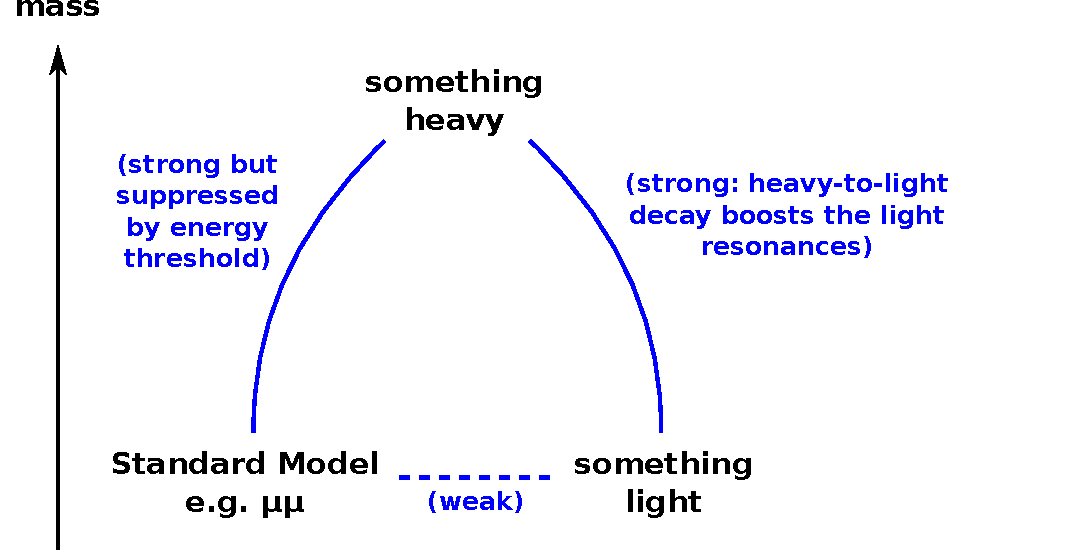
\includegraphics[width=0.9\linewidth]{basic_picture.pdf}}
\only<2>{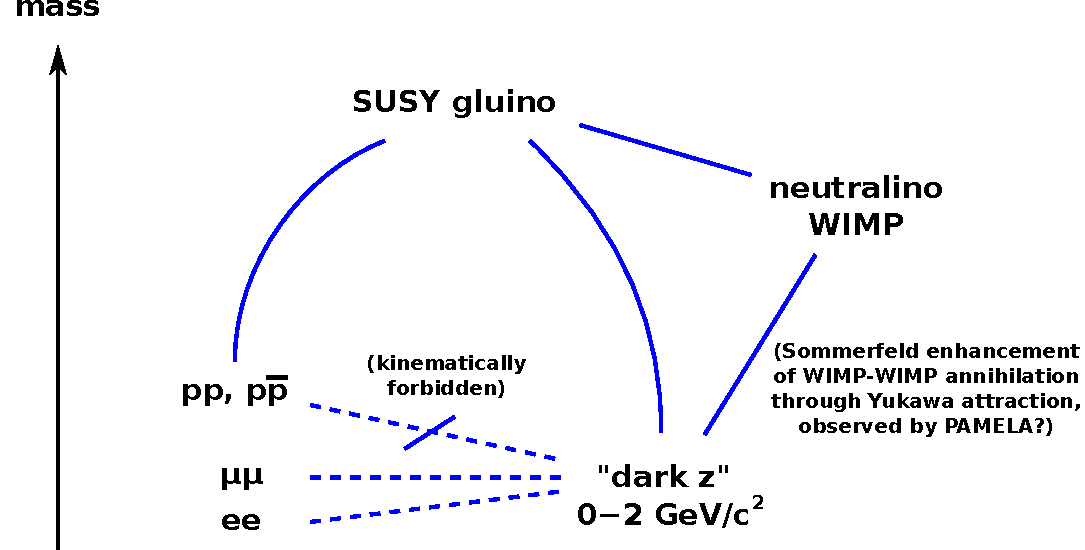
\includegraphics[width=0.9\linewidth]{basic_picture2.pdf}}
\only<3>{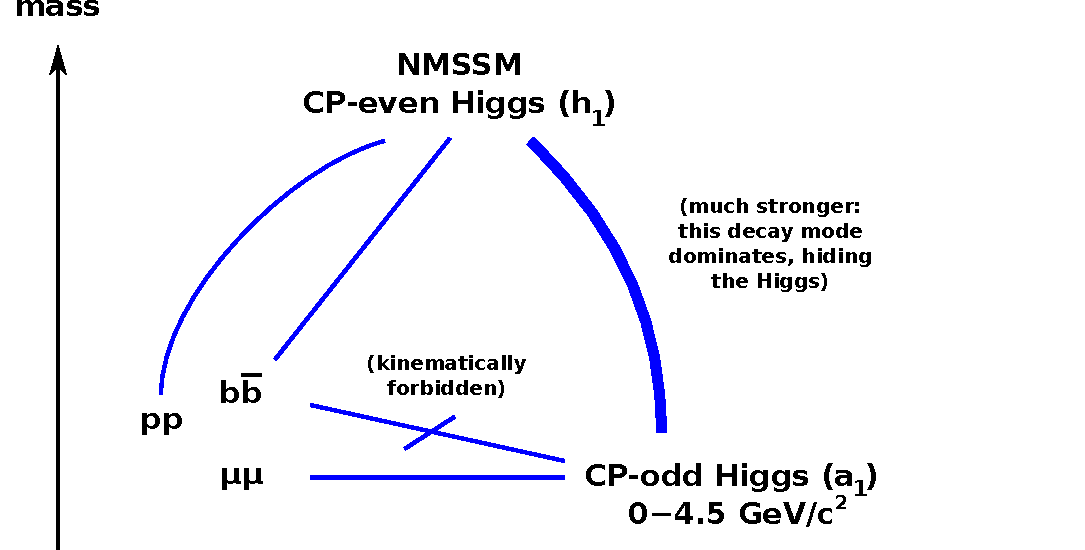
\includegraphics[width=0.9\linewidth]{basic_picture3.pdf}}
\end{center}

\begin{itemize}
\item \only<1>{Generic hidden-valley picture: predicts low-mass, high-momentum new particles}\only<2>{Special case motivated by PAMELA positron excess (and no antiproton excess) when interpreted as WIMP-WIMP annihilation}\only<3>{A region of NMSSM parameter space allows the Higgs to escape LEP limits; same basic picture, same signature}
\item<3> This was the first case our group studied: $h_1 \to a_1 a_1 \to 2\mu \, 2\mu$
\item<3> Topology motivates mass-peak fit in ``$2\mu$ mass vs.\ $2\mu$
  mass'' plane to find a bump corresponding to the $a_1$ mass
  \hfill {\scriptsize (hep-ex/1002.1956)}
\end{itemize}
\end{frame}

\begin{frame}
\frametitle{What we're looking for}

\begin{center}
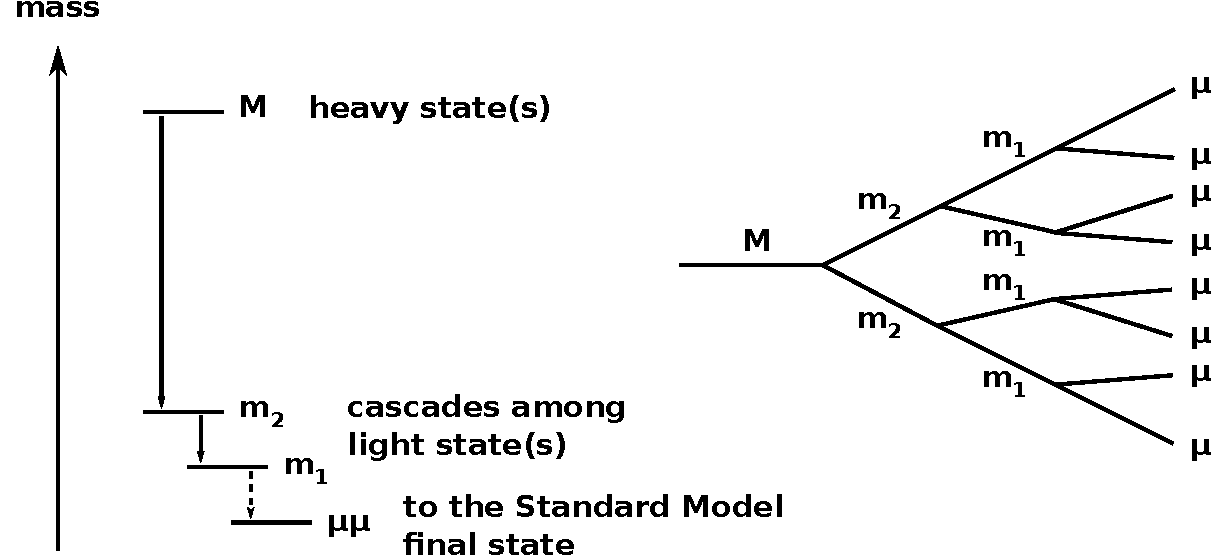
\includegraphics[width=0.8\linewidth]{basic_picture4.pdf}
\end{center}

\begin{itemize}
\item Since we don't know the physics of the hidden sector, we can't
  rule out complex decay chains leading to ``jets'' of \mbox{$\mu^+\mu^-$ (and
  $e^+e^-$, $\pi\pi$)\hspace{-0.5 cm}}
\item Assuming that the $m_i \cdot \gamma$ couplings are much weaker
  than the $m_i \cdot m_j$ couplings, cascades will need to decay down
  to the bottom of the chain before the slow transition to the
  Standard Model: this implies that all of the muon pairs come from
  $m_1$ decays
\item We're looking for \underline{\it one} new $m_1 \to \mu^+\mu^-$ resonance,
  possibly many instances per event, possibly overlapping
\end{itemize}
\end{frame}

\begin{frame}
\frametitle{Analysis method}
\begin{itemize}
\item The basic problem is combinatoric: identify which opposite-sign
  muon pairs belong to which $m_1$ decays, and then look for an $m_1$
  dimuon mass peak by fitting all of them
\item Grouping neaby muons into ``jets'' helps to distinguish muons
  from different heavy $M$ decays and provides a classification scheme
  for different signal topologies with different backgrounds:
\begin{enumerate}[(\alph{enumi})]
\item exactly one mu-jet per event
\begin{enumerate}[(\mbox{a}-\arabic{enumii})]
\item mu-jet contains two muons with high momentum ($m_1 \to 2\mu$)
\item mu-jet contains four muons ($m_2 \to m_1 m_1 \to 4\mu$)
\item more than four
\end{enumerate}

\item two mu-jets per event
\begin{enumerate}[(b-\arabic{enumii})]
\item $2\mu$, $2\mu$ ($M \to m_1 m_1$, which is the NMSSM signature)
\item $2\mu$, $4\mu$ ($M \to m_1 m_2$)
\item $4\mu$, $4\mu$ ($M \to m_2 m_2$)
\item either has more than four
\end{enumerate}

\item more than two mu-jets per event
\end{enumerate}
\end{itemize}
\end{frame}

\begin{frame}
\frametitle{Analysis method}

\begin{columns}
\column{0.5\linewidth}
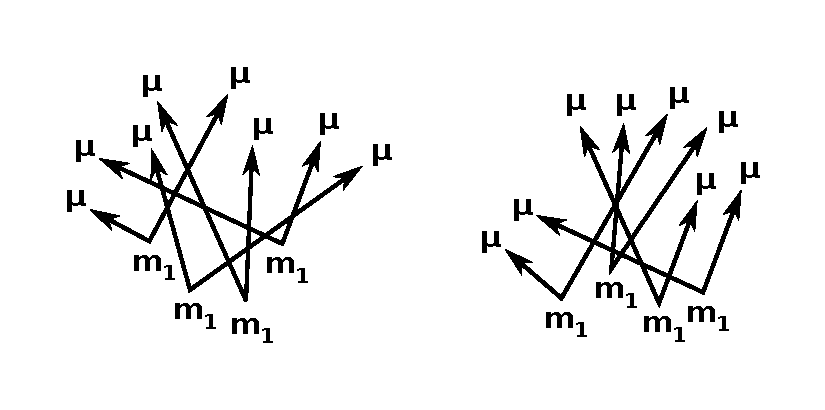
\includegraphics[width=\linewidth]{combinatorics.pdf}

\column{0.5\linewidth}
0. Start with a clean set of muons
\end{columns}

\begin{columns}
\column{0.5\linewidth}
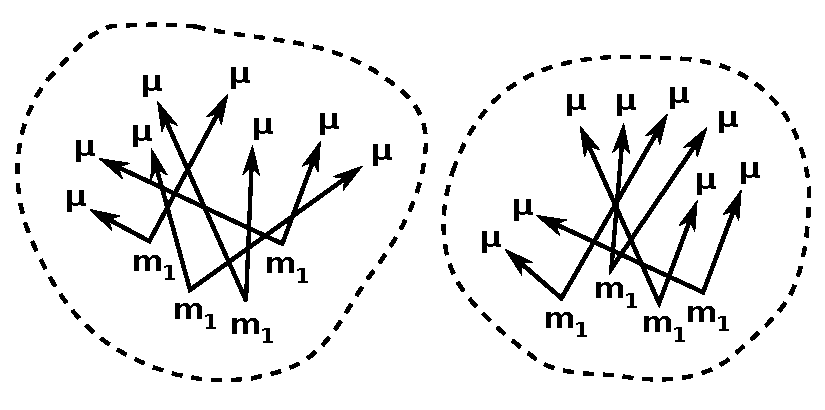
\includegraphics[width=\linewidth]{combinatorics2.pdf}

\column{0.5\linewidth}
1. Identify mu-jets by kinematics, rather than geometry (next slide), so
that everything within a mu-jet came from the decay of something
lighter than 5~GeV/$c^2$
\end{columns}

\begin{columns}
\column{0.5\linewidth}
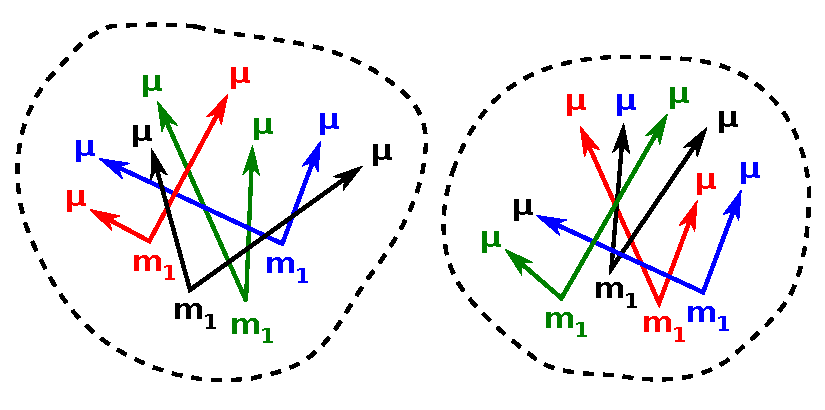
\includegraphics[width=\linewidth]{combinatorics3.pdf}

\column{0.5\linewidth}
2. Find the combination of pairs in which the dimuon masses are most consistent with being equal:

\mbox{ } \hfill $m_a \approx m_b \approx m_c \approx m_d$ \hfill \mbox{ }

\vspace{0.2 cm}
3. $N$-D fit to the dimuon masses
\end{columns}
\end{frame}

\begin{frame}
\frametitle{Analysis method}

\begin{itemize}
\item Put two muons in the same mu-jet if
\[ \left( m_\s{pair} < 5\mbox{ GeV/$c^2$ {\bf and} }P_\s{vertex} > 0.01\right)\mbox{ {\bf or} }\Delta R < 0.01 \]

\item Sensitive to a rectangular region in the ($p_T$, mass) plane
\begin{itemize}
\item the signal would be a narrow vertical smear on this plane
\end{itemize}
\end{itemize}

\begin{center}
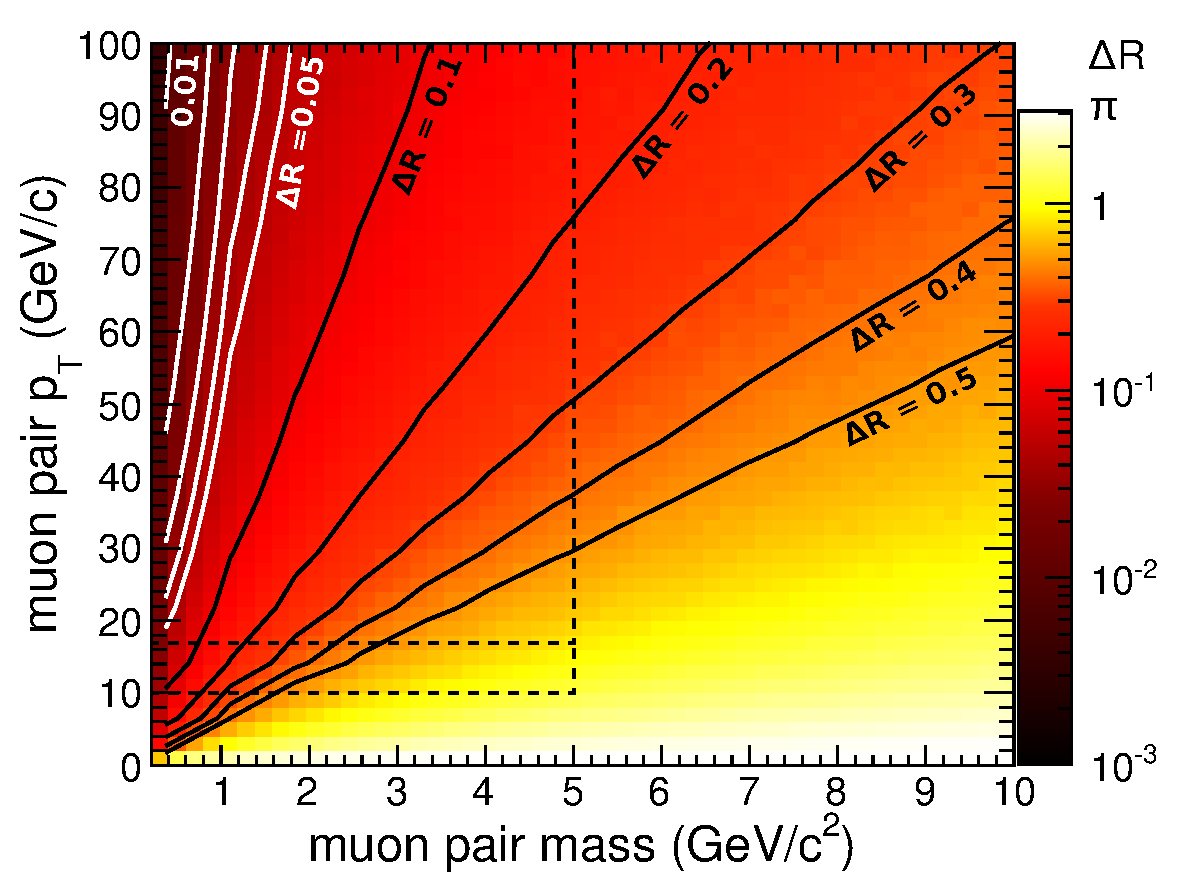
\includegraphics[width=0.7\linewidth]{openingangle_dr.pdf}
\end{center}
\end{frame}

\begin{frame}
\frametitle{Analysis method}
\begin{itemize}
\item After grouping muons into mu-jets (step 1) and decomposing them
  into fundamental dimuons (step 2), we have $N$ dimuons per event

  (value of $N$ depends on the subsample, categorized by mu-jets)

\item Fit background and potential signal to a single ansatz: signal
  must be on the diagonal because $m_a \approx m_b \approx m_1$

\begin{center}
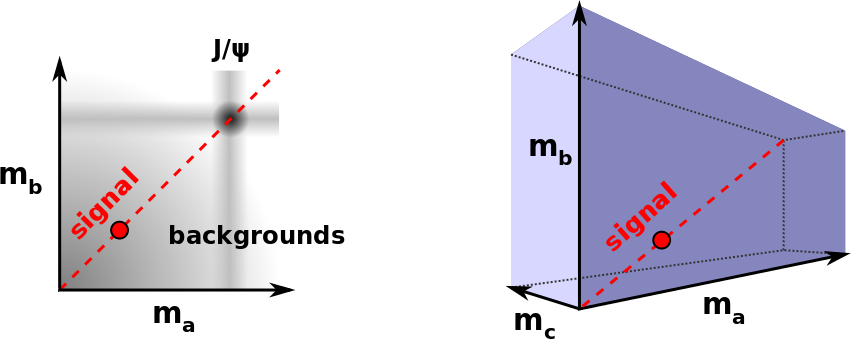
\includegraphics[width=0.9\linewidth]{diagonal.png}
\end{center}

\item Shape of background comes from control samples, normalization
  is fitted simultaneously with the signal (like any bump-hunt)
\end{itemize}
\end{frame}

\begin{frame}
\frametitle{Analysis method}
\textcolor{darkblue}{Background templates are different for each signal channel}
\begin{enumerate}[(\alph{enumi})]
\item exactly one mu-jet per event
\begin{enumerate}[(\mbox{a}-\arabic{enumii})]
\item mu-jet contains two muons with high momentum
\begin{itemize}
\item \textcolor{darkblue}{backgrounds:} $p_T$ tails of Standard Model dimuon resonances
\item \textcolor{darkblue}{control:} dimuons of intermediate momentum
\end{itemize}

\item mu-jet contains four muons
\item more than four $(n)$
\begin{itemize}
\item \textcolor{darkblue}{backgrounds:} physical dimuon with fake
  muons attached
\item \textcolor{darkblue}{control:} two muons + $(n-2)$ tracks
\end{itemize}
\end{enumerate}

\item two mu-jets per event
\begin{enumerate}[(b-\arabic{enumii})]
\item $2\mu$, $2\mu$
\begin{itemize}
\item \textcolor{darkblue}{backgrounds:} $b\bar{b}$ with each $b \to 2\mu X$ (semileptonic or fake)
\item \textcolor{darkblue}{control:} $b \to 2\mu X$ dimuons (isolation, displaced vertex) \\
carefully account for trigger bias in one of the dimuons
\end{itemize}

\item $2\mu$, $4\mu$
\item $4\mu$, $4\mu$
\item either has more than four
\begin{itemize}
\item combinations of the above
\end{itemize}
\end{enumerate}

\item more than two mu-jets per event: {\scriptsize more combinations of the above}
\end{enumerate}
\end{frame}

\begin{frame}
\frametitle{Analysis method}
\begin{itemize}
\item Acceptance cuts:
\begin{itemize}
\item at least one $p_T > 12$~GeV/$c$, $|\eta| < 0.9$ muon (trigger plateau)
\item all other muons have $p_T > 5$~GeV/$c$, $|\eta| < 2.4$ (reco plateau)
\item signal regions defined by number of mu-jets and number of muons in mu-jets
\end{itemize}

\item No analysis cuts on isolation
\begin{itemize}
\item $m_1 \to e^+e^-$, $\pi\pi$ are just as possible as $m_1 \to \mu^+\mu^-$, so isolation doesn't sequester the signal
\item there may be hadronic jets nearby from SUSY decays
\end{itemize}

\item No cuts on missing energy, hadronic jets, isolated leptons,
  etc. (they're neither required nor rejected)

\item All data-driven backgrounds come from fits for normalization and control samples for shapes

\item Signal peak resolution from data (fit to $\omega$, $\phi$, $J/\psi$, and $\psi'$)

\item Single-valued or $\eta$-dependent efficiency correction from $Z$
  tag-and-probe: regions with complicated efficiency dependence have
  already been rejected with acceptance cuts
\end{itemize}
\end{frame}

\begin{frame}
\frametitle{Study of low-$p_T$ dimuon control}

\begin{itemize}
\item In the next few slides, we'll take a close look at single-dimuon events
  with vector-sum $p_T < 80$~GeV/$c$
\begin{itemize}
\item Standard Model dominates over potential $\mathcal{O}(\mbox{1 pb})$ signals (determined by Monte Carlo before looking at data)
\end{itemize}

\item It will be important to understand this distribution well enough
  to know what physics produced it and which processes will be active
  in the signal regions, to make the right extrapolations

\hfill 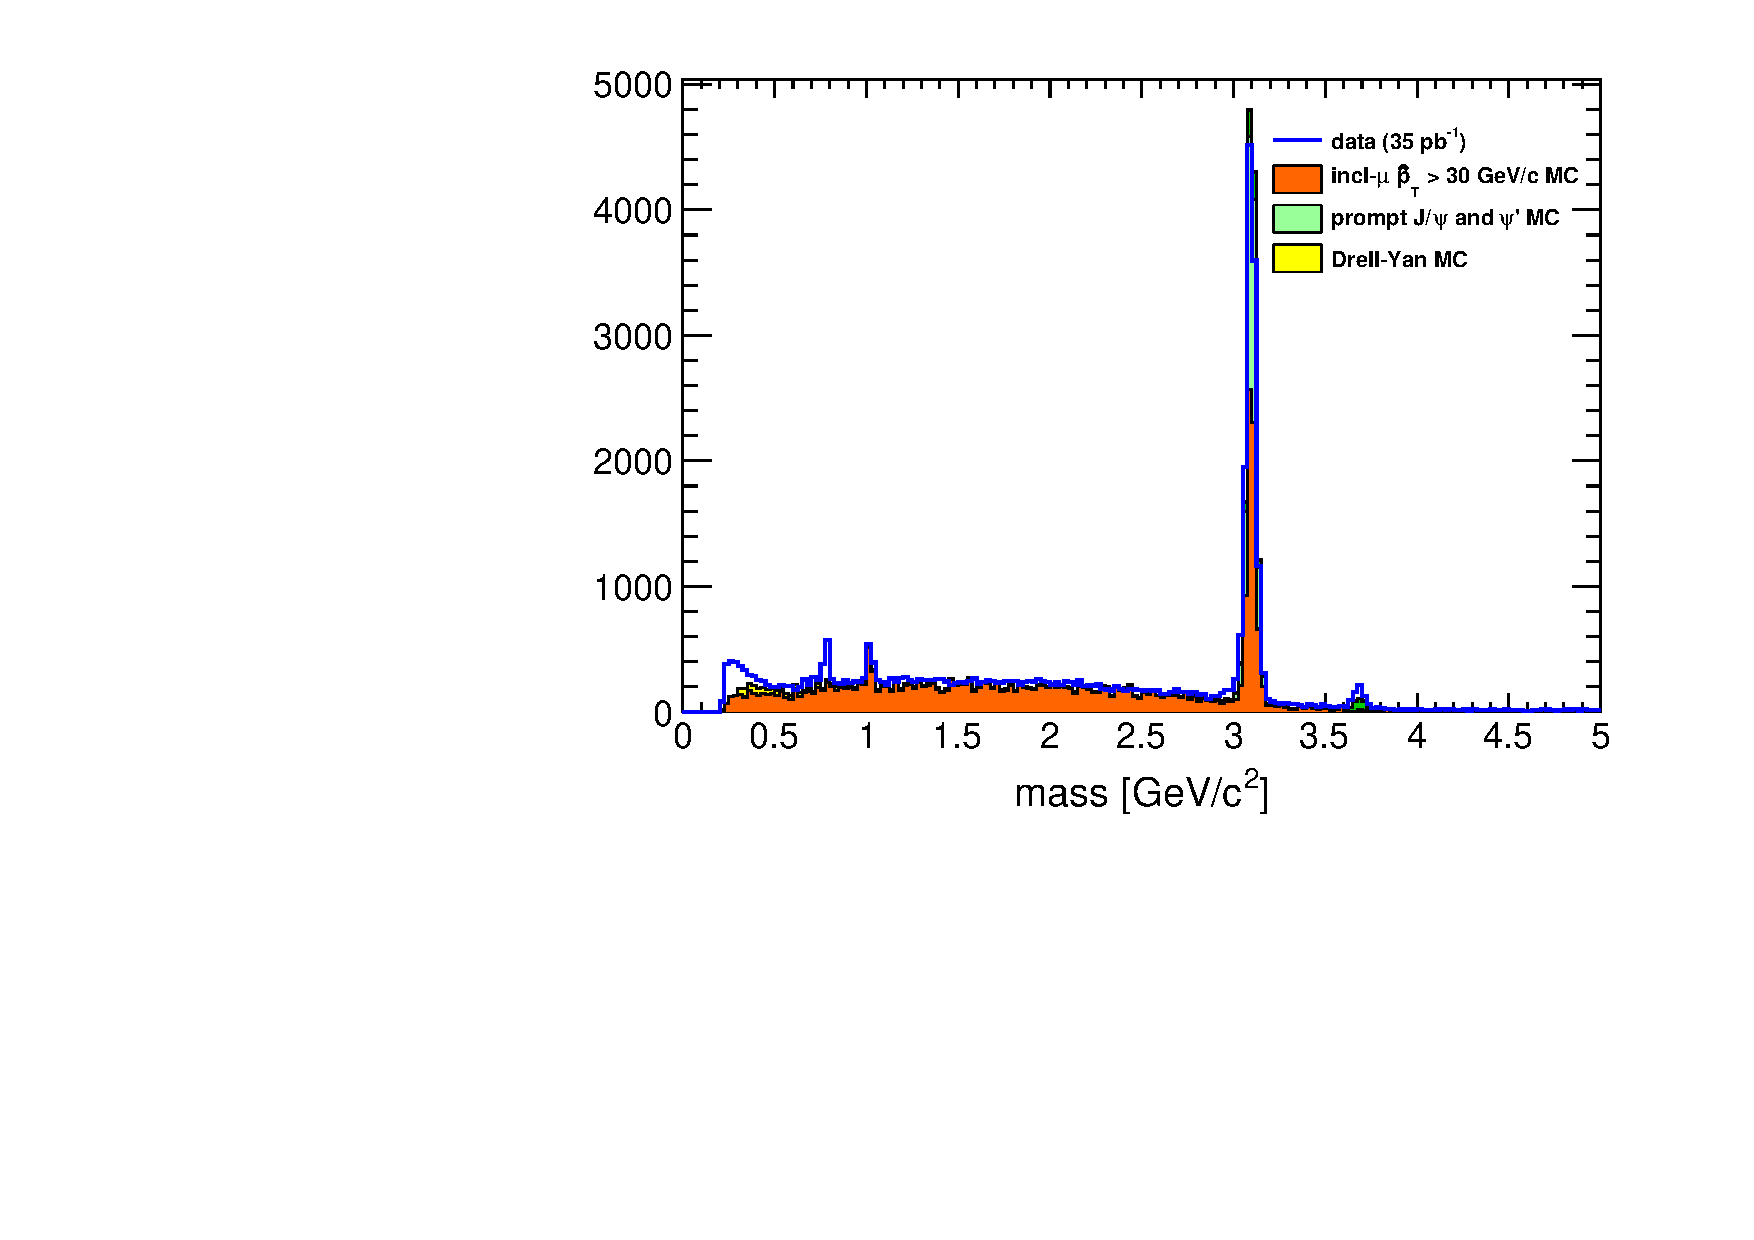
\includegraphics[width=0.6\linewidth]{lowdimuon_massdistribution.pdf}

\vspace{-4.2 cm}
\item Monte Carlos: inclusive- \\ muon ($\hat{p}_T > 30$~GeV/$c$), \\ prompt $J/\psi$, $\psi'$, and \\ privately-generated low-\\ mass Drell-Yan \\ ($\hat{p}_T > 10$~GeV/$c$, Pythia8 \\ to avoid a hard cut-off \\ in Pythia6)
\end{itemize}
\end{frame}

\begin{frame}
\frametitle{Study of low-$p_T$ dimuon control}

\begin{itemize}
\item Inclusive-muon MC is missing resonances: $\psi'$, $\omega$, and possibly $\eta \to \mu\mu\gamma$ ($\eta$ mass is 0.5~GeV/$c^2$, need to reconstruct $\gamma$ to be sure)
\item Inclusive-muon and $\psi'$ are normalized to their
  Pythia-calculated cross-sections, $J/\psi$ is normalized to its mass
  peak, and Drell-Yan is normalized to the $Z$
\end{itemize}

\begin{center}
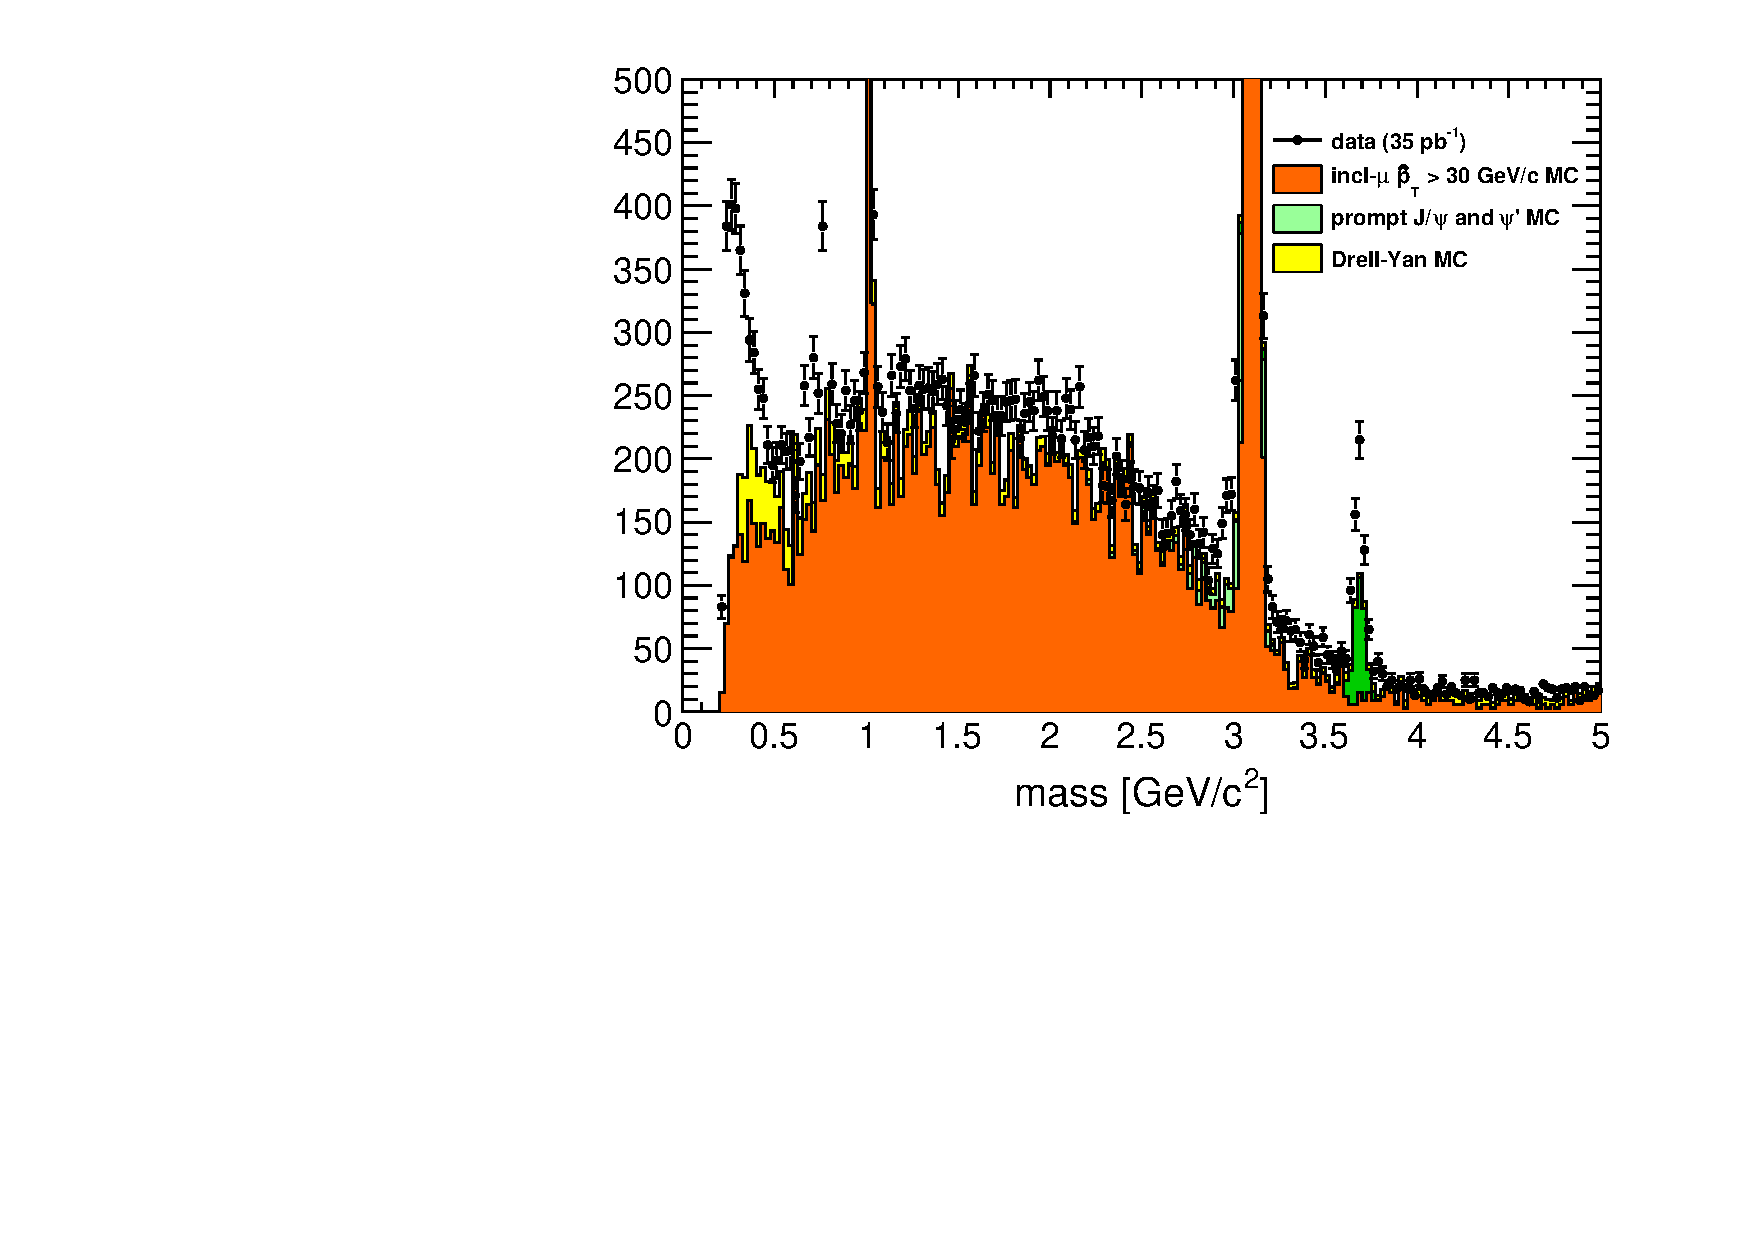
\includegraphics[width=0.8\linewidth]{lowdimuon_mass_nobcuts.pdf}
\end{center}
\end{frame}

\begin{frame}
\frametitle{Study of low-$p_T$ dimuon control}

\begin{itemize}
\item Isolation variable to study this sample:
\[ Iso = \sum_\s{tracks} p_T \mbox{ if } p_T > 1.5\mbox{ GeV/$c$, } \Delta R < 0.4 \mbox{, and \underline{not a muon}} \]

\item Minimum $p_T$ avoids dependence on pile-up (MC-tested)

\item Optimized to give a flat region in inclusive-muon MC near zero
\end{itemize}

\begin{center}
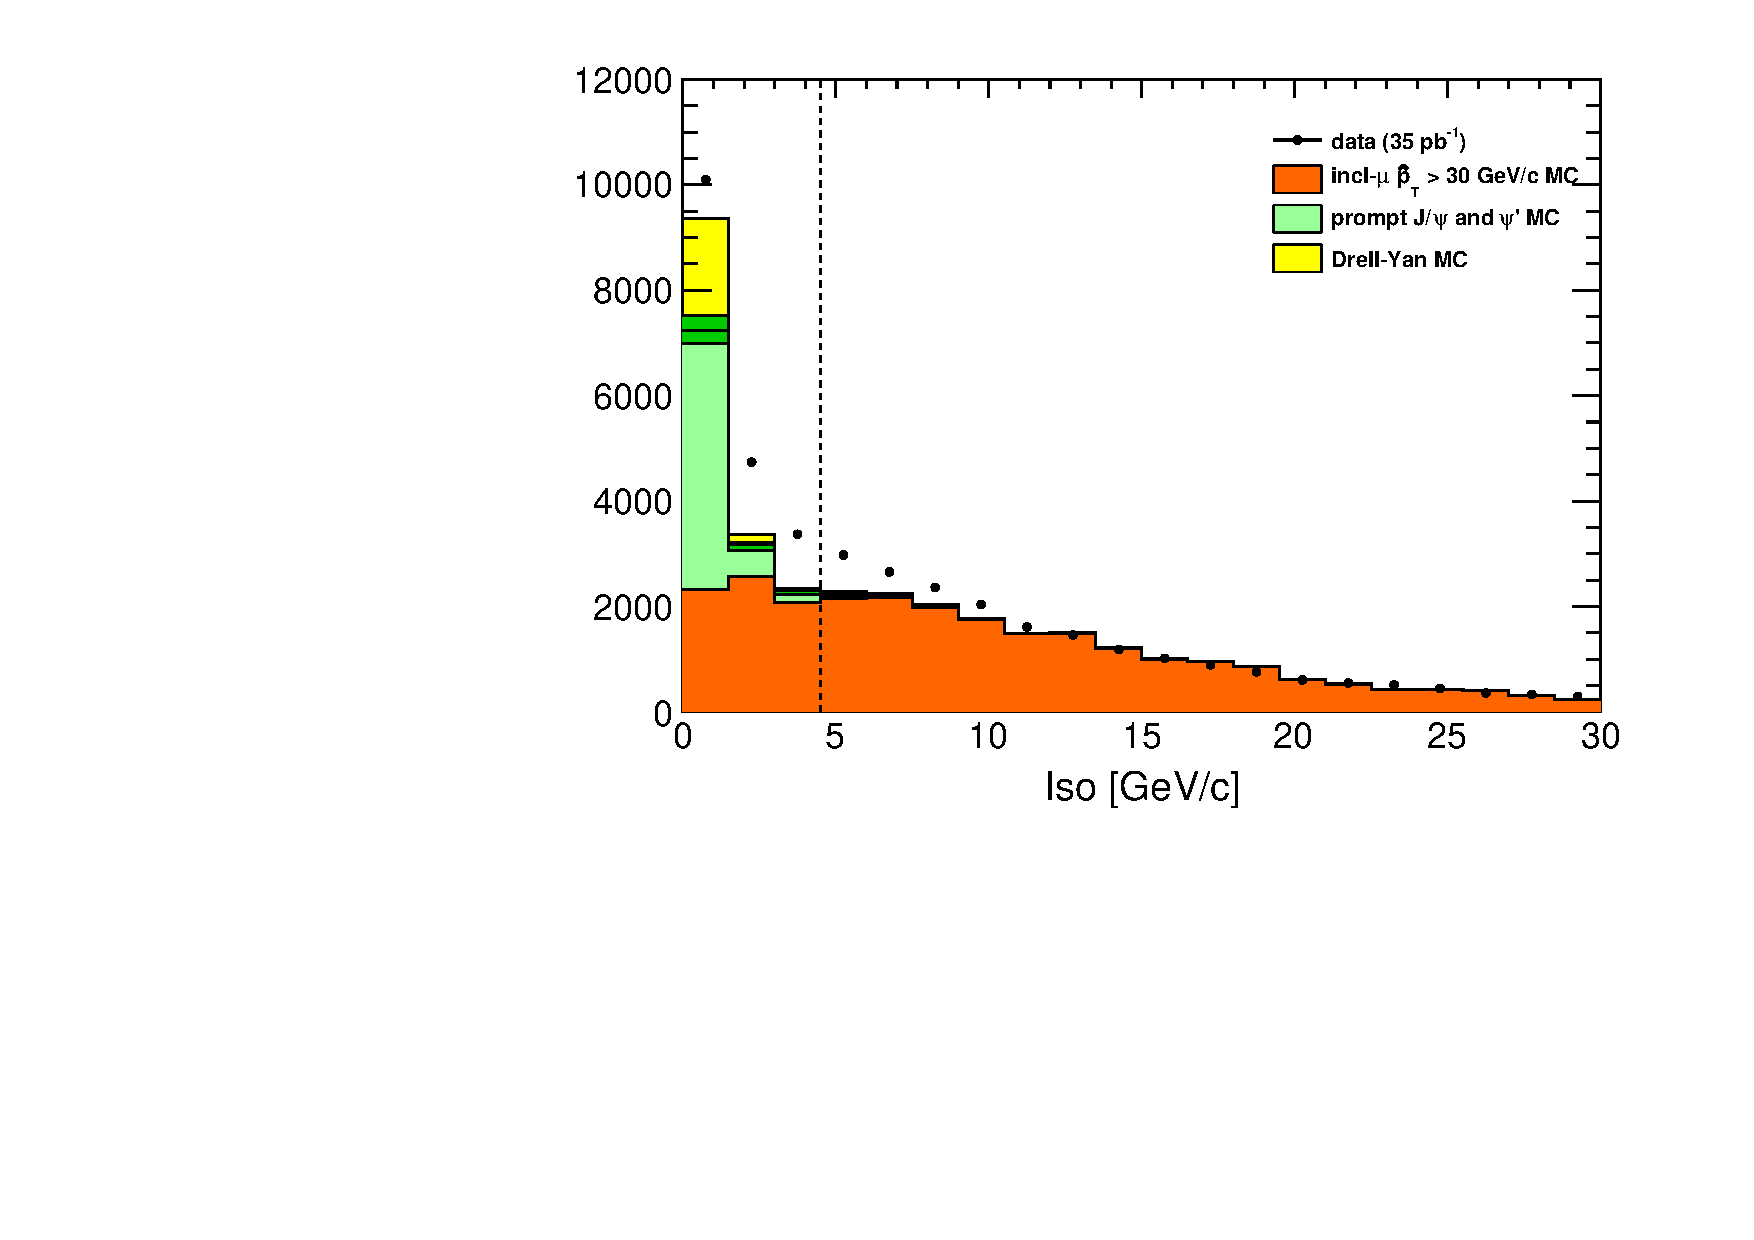
\includegraphics[width=0.75\linewidth]{lowdimuon_iso_everything.pdf}
\end{center}
\end{frame}

\begin{frame}
\frametitle{Study of low-$p_T$ dimuon control}

\begin{columns}
\column{0.5\linewidth}
\begin{itemize}
\item Plots of mass with \mbox{isolation cuts\hspace{-1 cm}}
\item Non-isolated regions can be described by inclusive-muon and the missing resonances
\item Isolated component is missing a continuum of mid-range masses
\end{itemize}

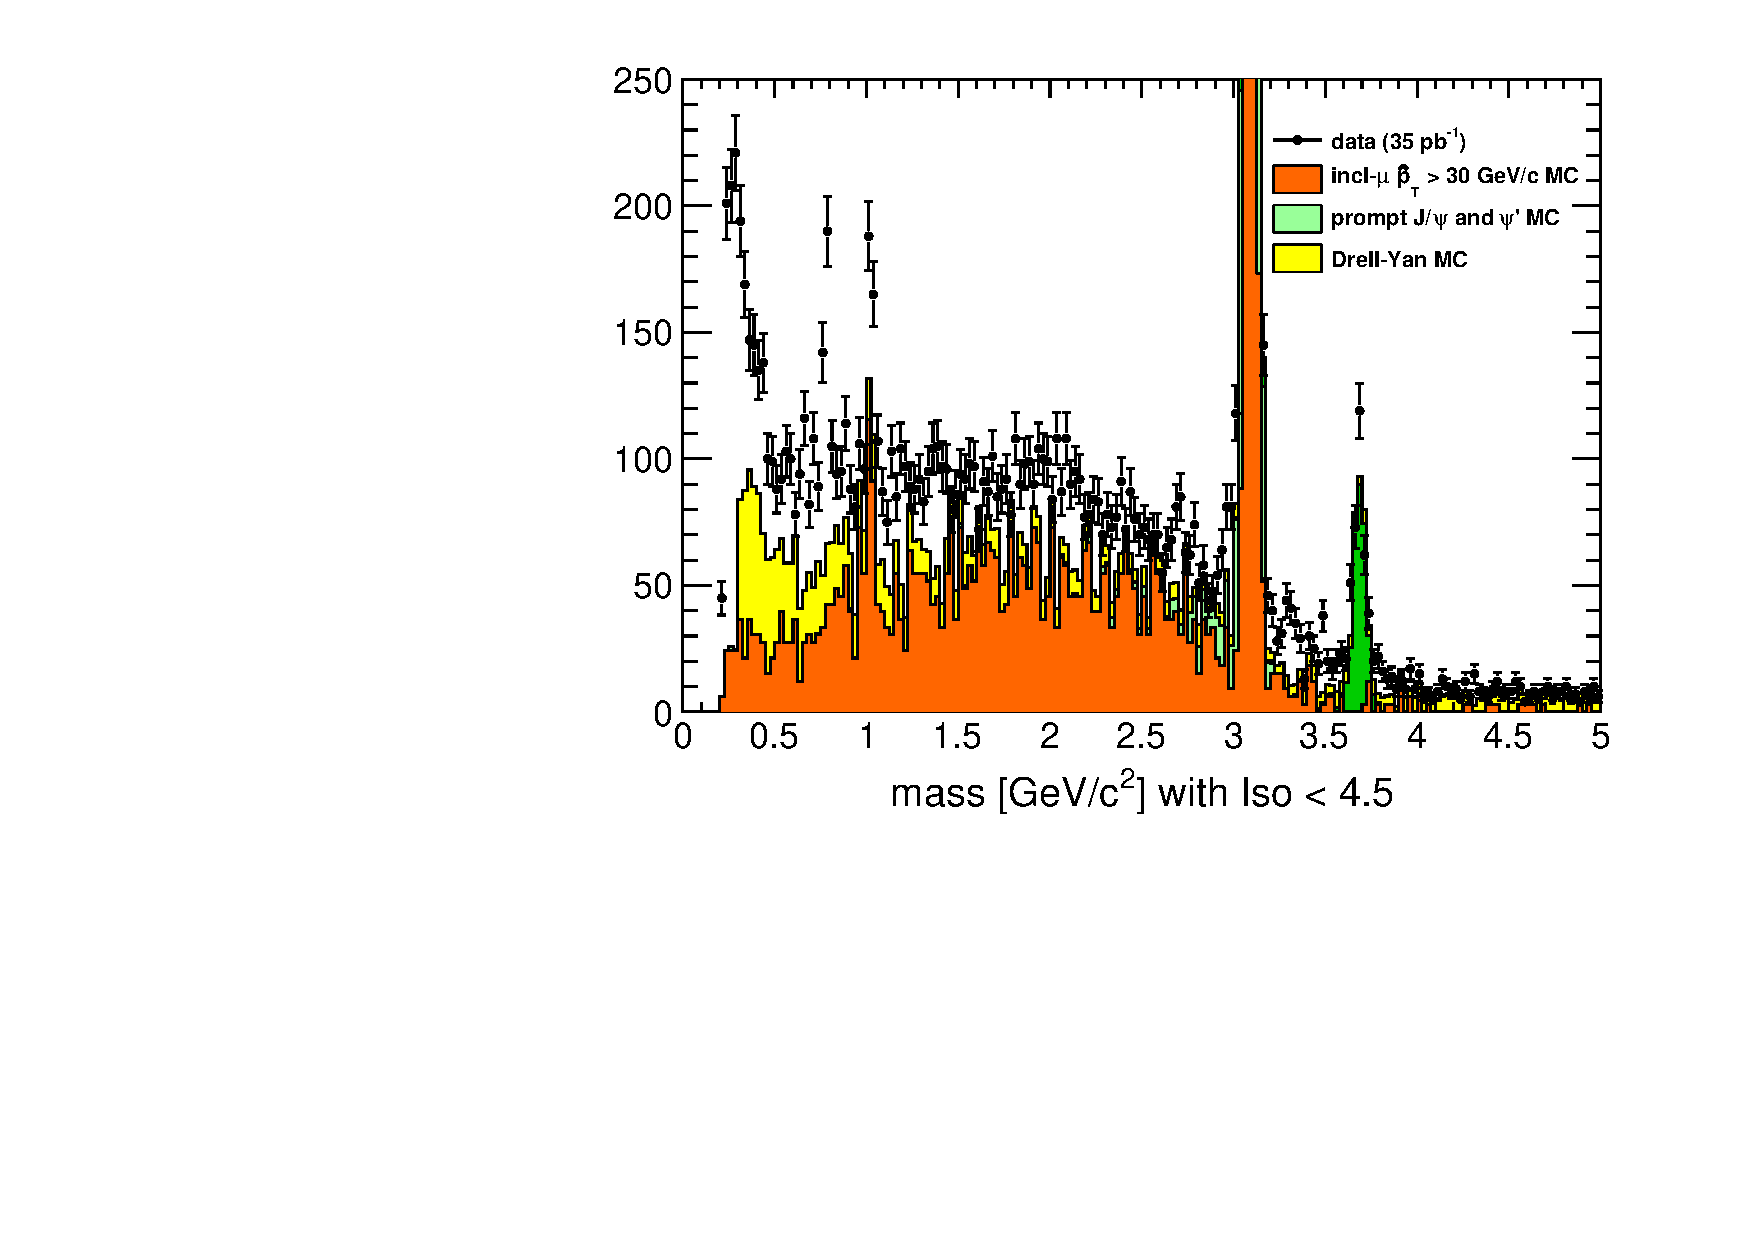
\includegraphics[width=1.2\linewidth]{lowdimuon_mass_isolated.pdf}

\column{0.5\linewidth}
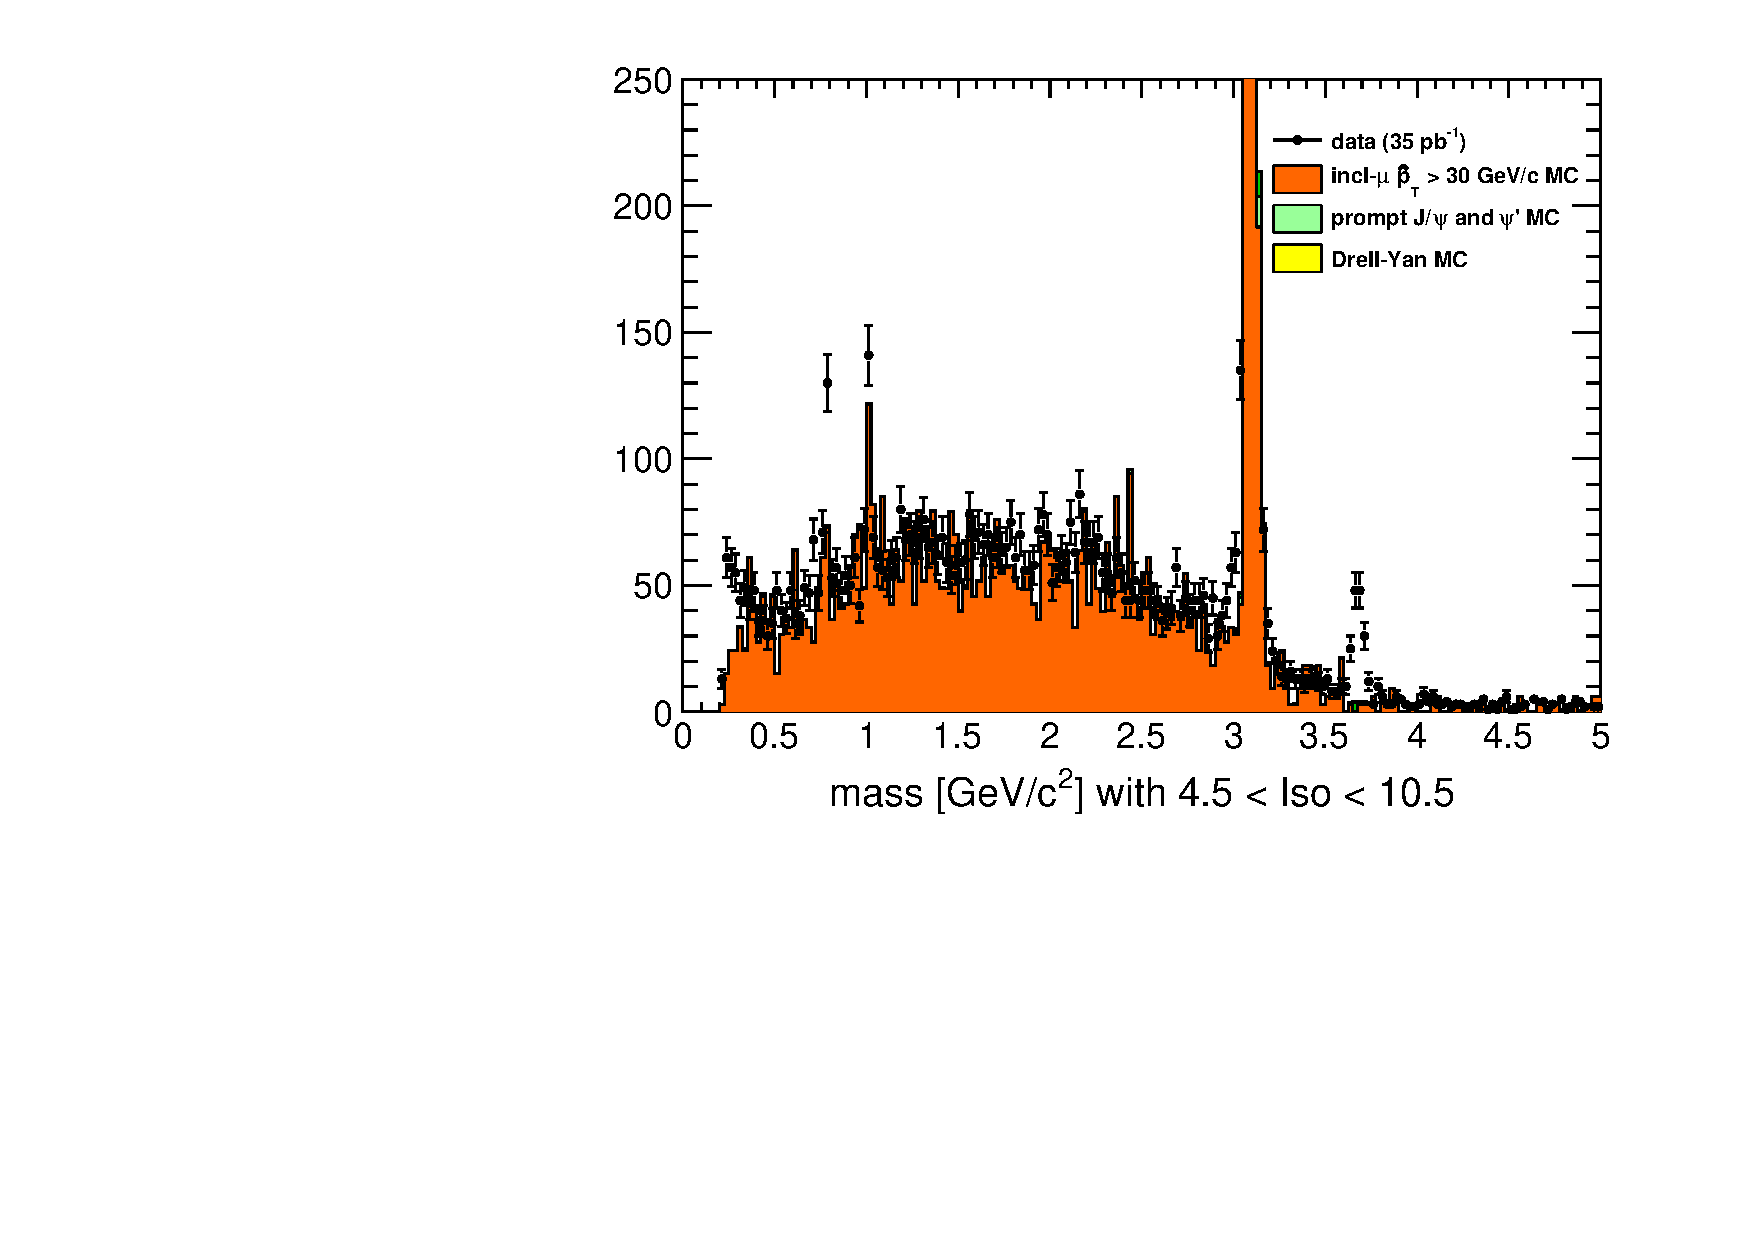
\includegraphics[width=\linewidth]{lowdimuon_mass_isosideband.pdf}

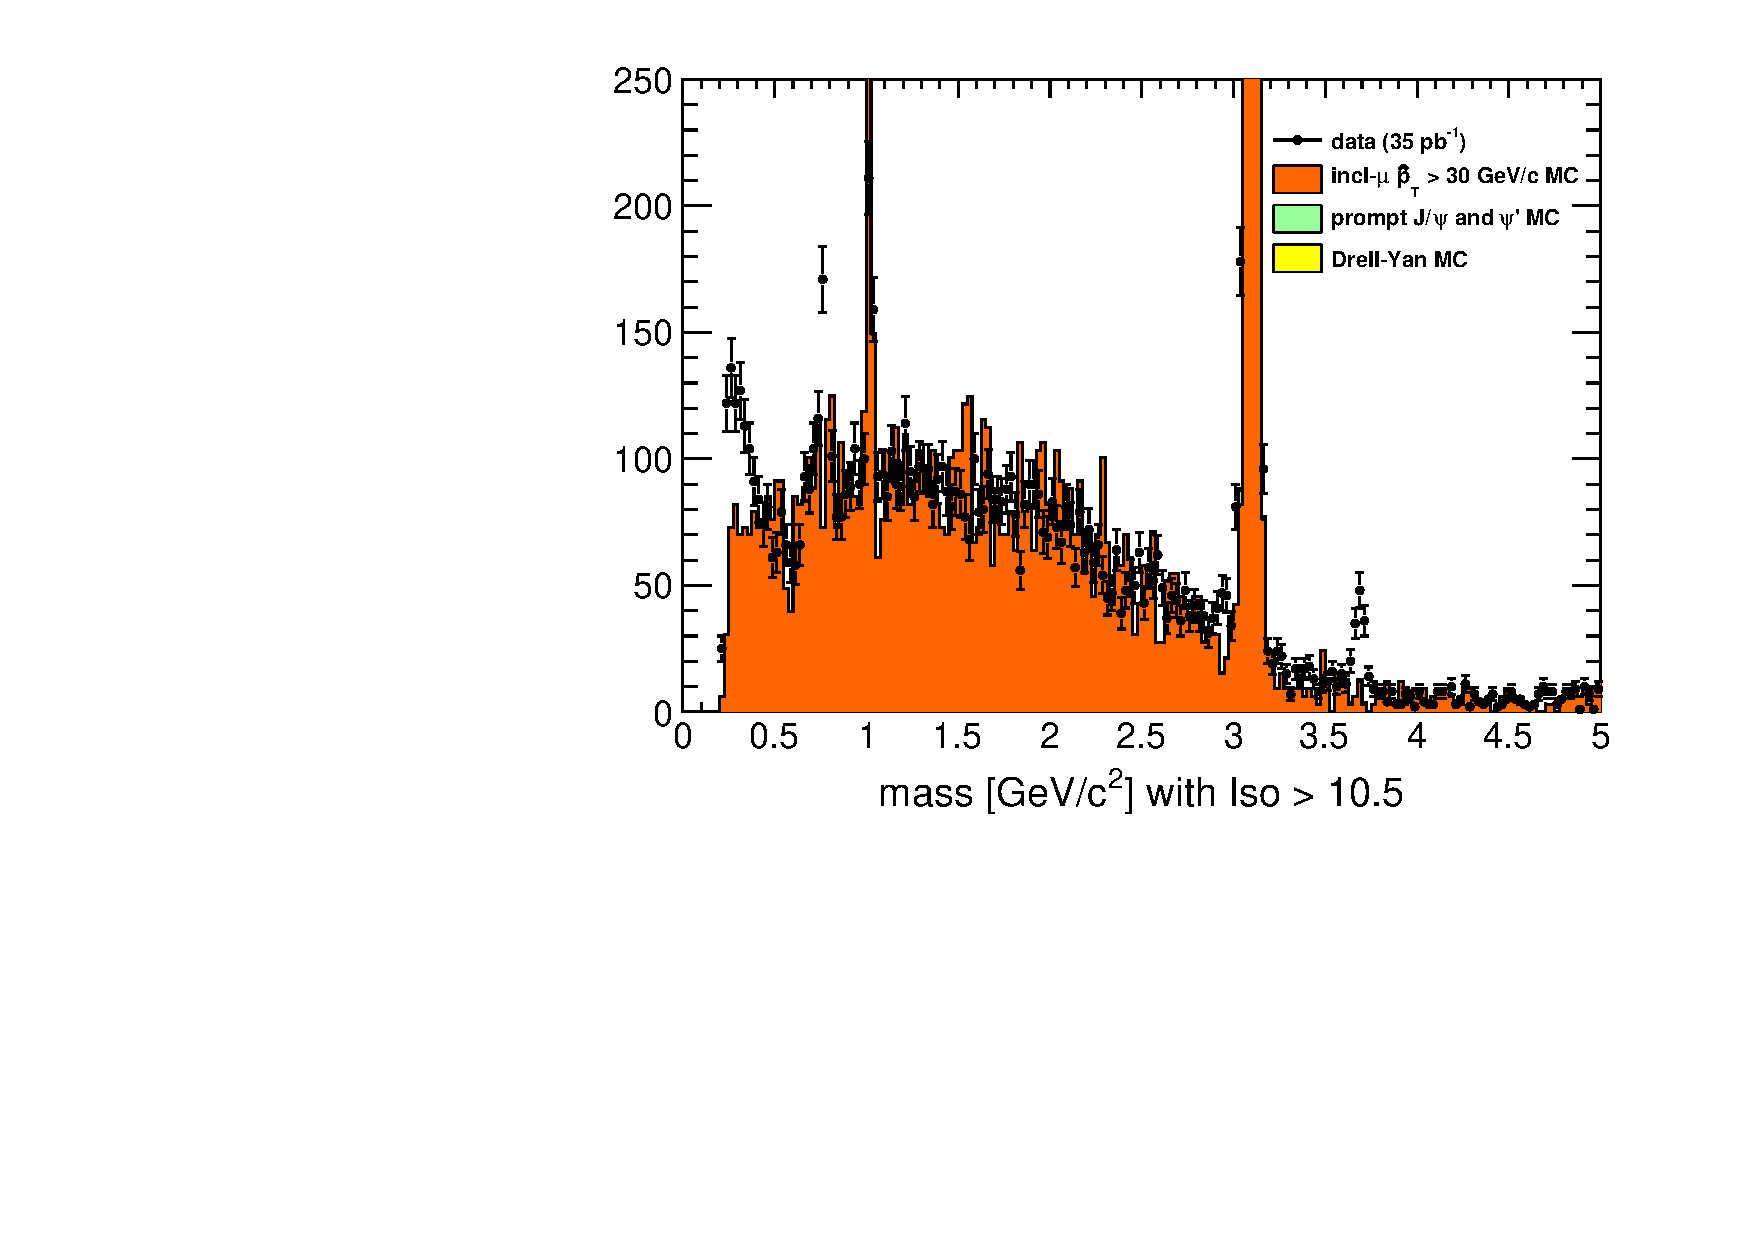
\includegraphics[width=\linewidth]{lowdimuon_mass_noniso.pdf}
\end{columns}
\end{frame}

\begin{frame}
\frametitle{Study of low-$p_T$ dimuon control}

\begin{columns}
\column{0.5\linewidth}
\begin{itemize}
\item $L_{xy}$: displacement of dimuon vertex from primary vertex in
  the $x$-$y$ direction of flight
\item Missing isolated continuum in mid-range masses is displaced with
  a smaller $(\gamma c\tau)_T$ than incl-$\mu$ MC: qualitatively con- sistent with
  \mbox{$\hat{p}_T < 30$~GeV/$c$ $b\bar{b}$\hspace{-1 cm}}
\end{itemize}

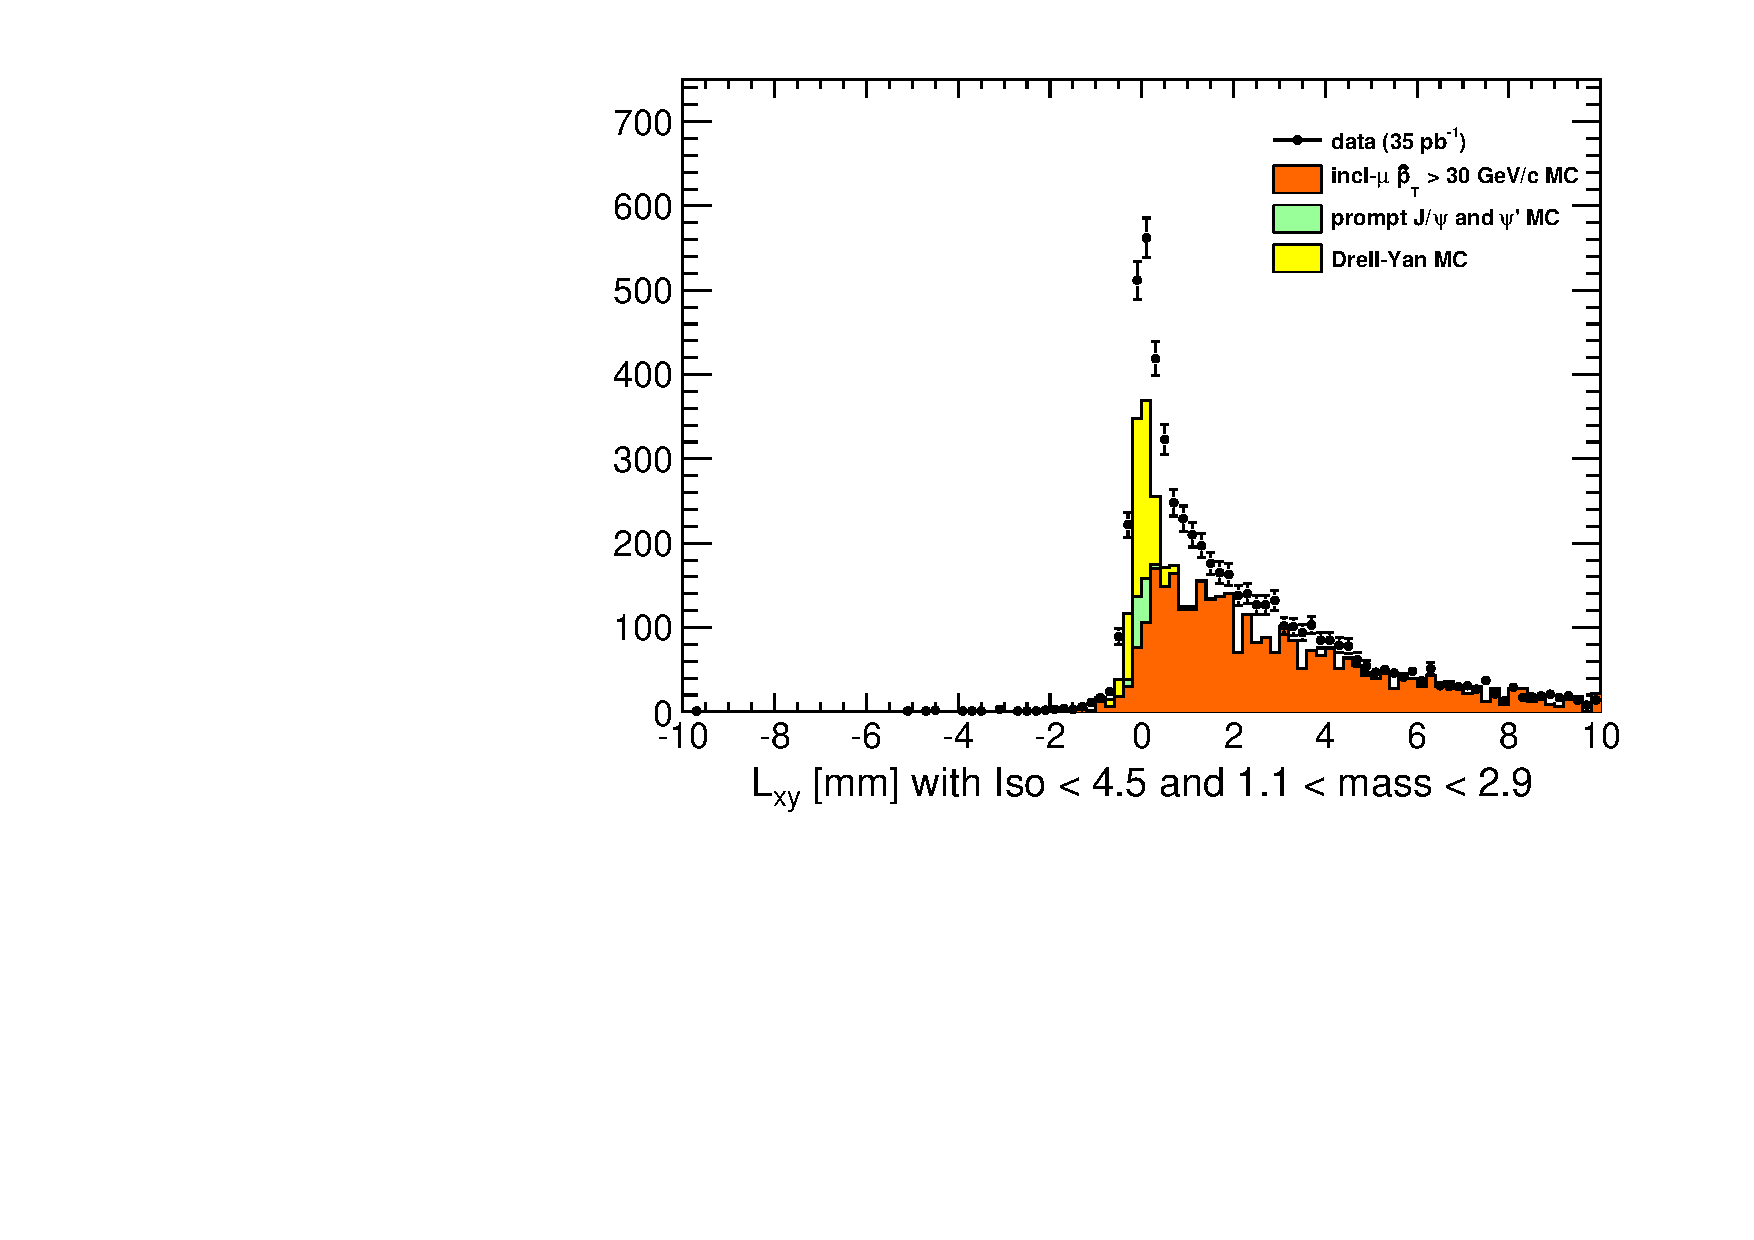
\includegraphics[width=1.2\linewidth]{lowdimuon_lxy_midmass_isolated.pdf}

\column{0.5\linewidth}
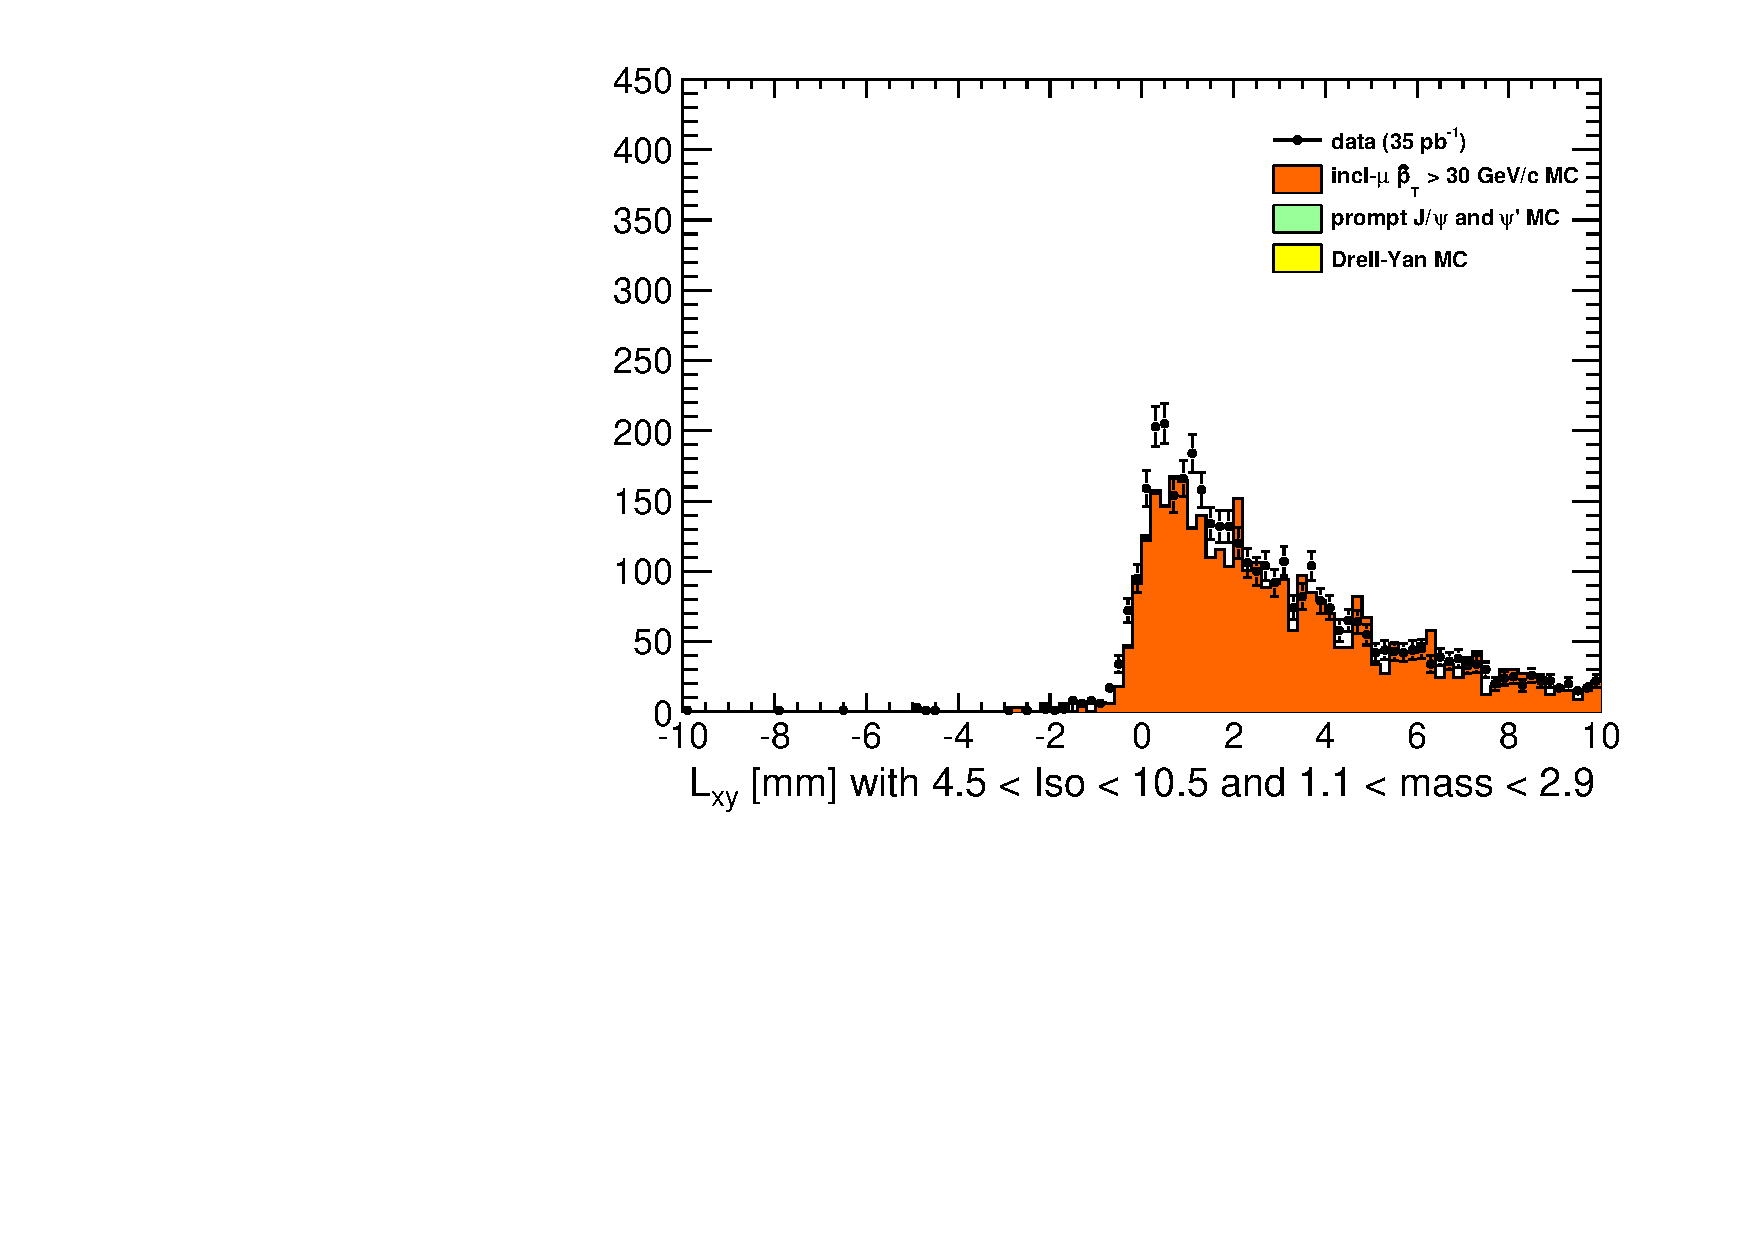
\includegraphics[width=\linewidth]{lowdimuon_lxy_midmass_isosideband.pdf}

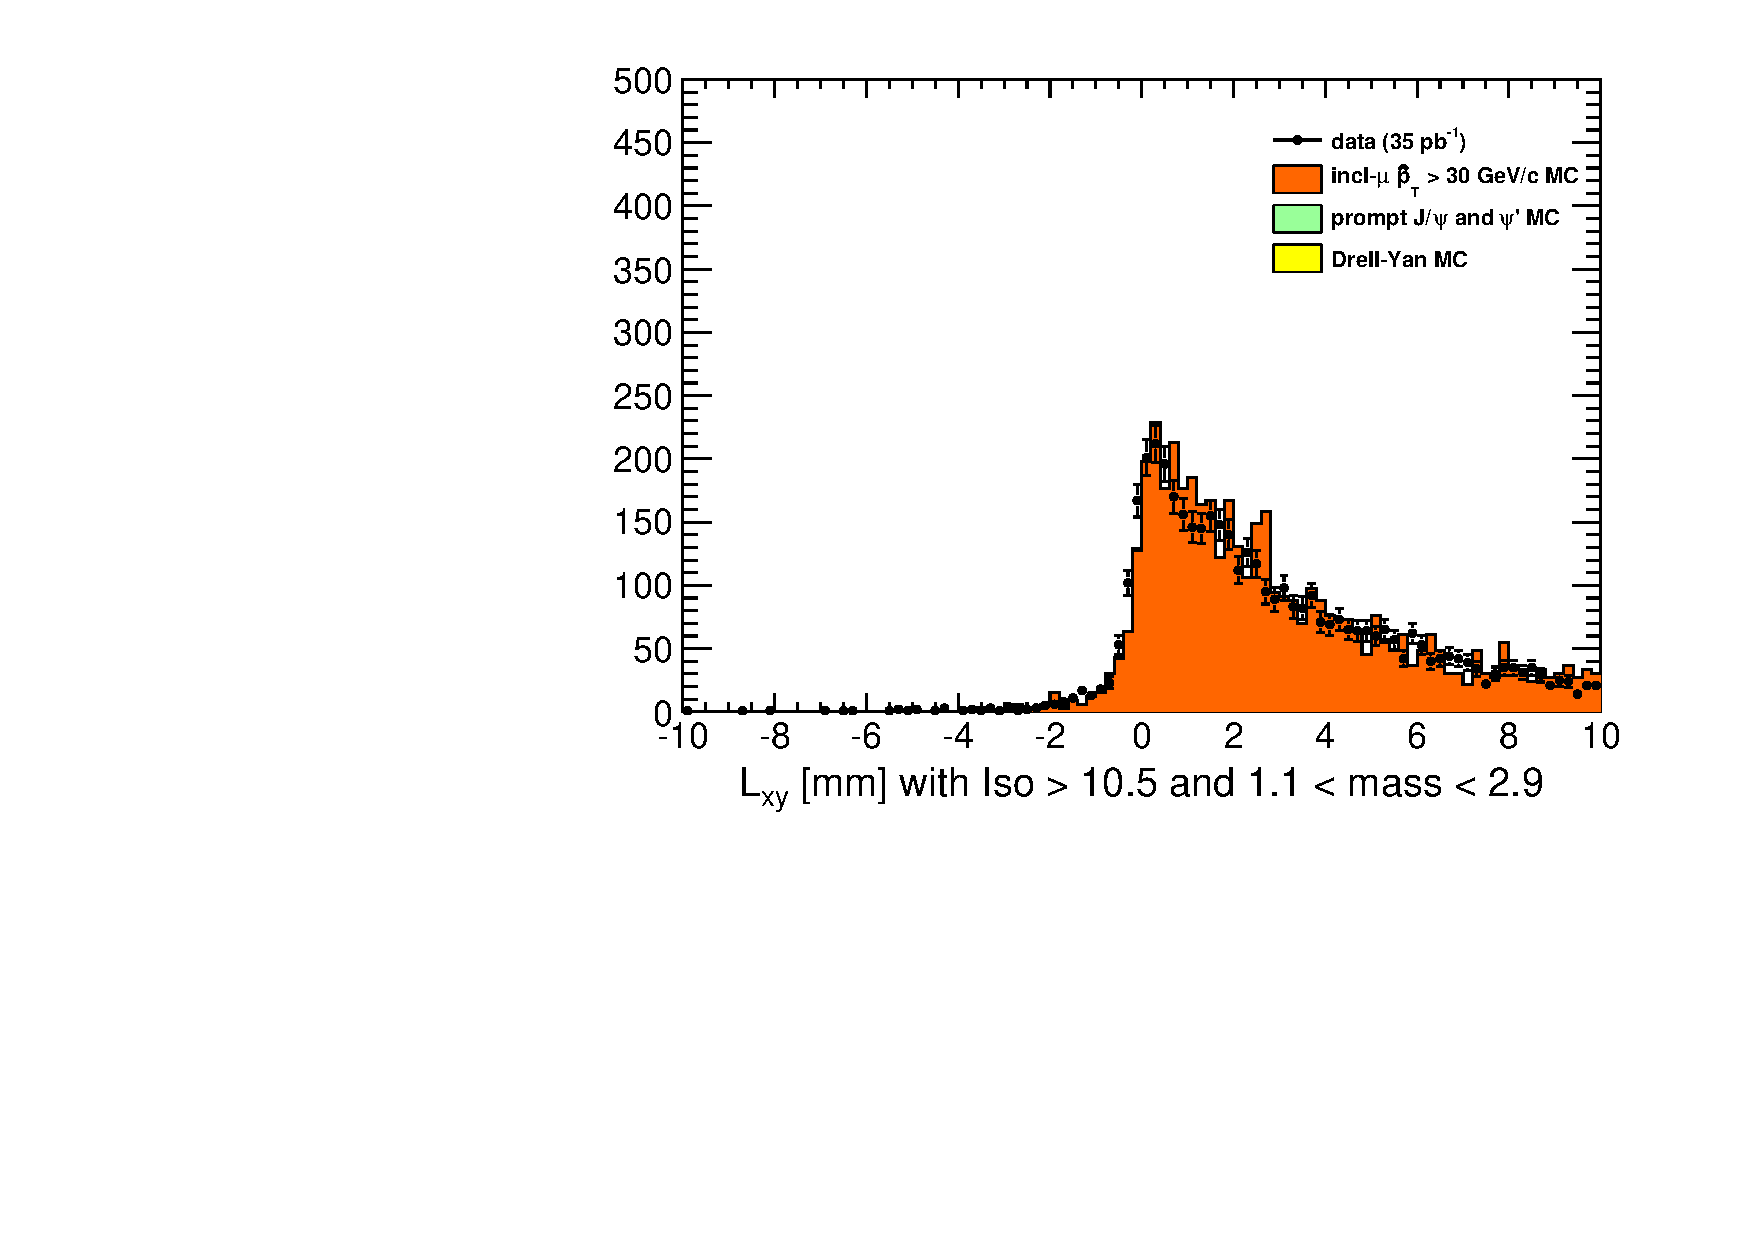
\includegraphics[width=\linewidth]{lowdimuon_lxy_midmass_noniso.pdf}
\end{columns}
\end{frame}

\begin{frame}
\frametitle{Study of low-$p_T$ dimuon control}

\begin{columns}
\column{0.5\linewidth}
\begin{itemize}
\item Low-mass excess is inconclusive in $L_{xy}$ because vertex
  resolution for nearly collinear muons is poor
\item However, they're definitely not $\gamma \to \mu\mu$ conversions
  (the beampipe is at 30~mm)
\end{itemize}

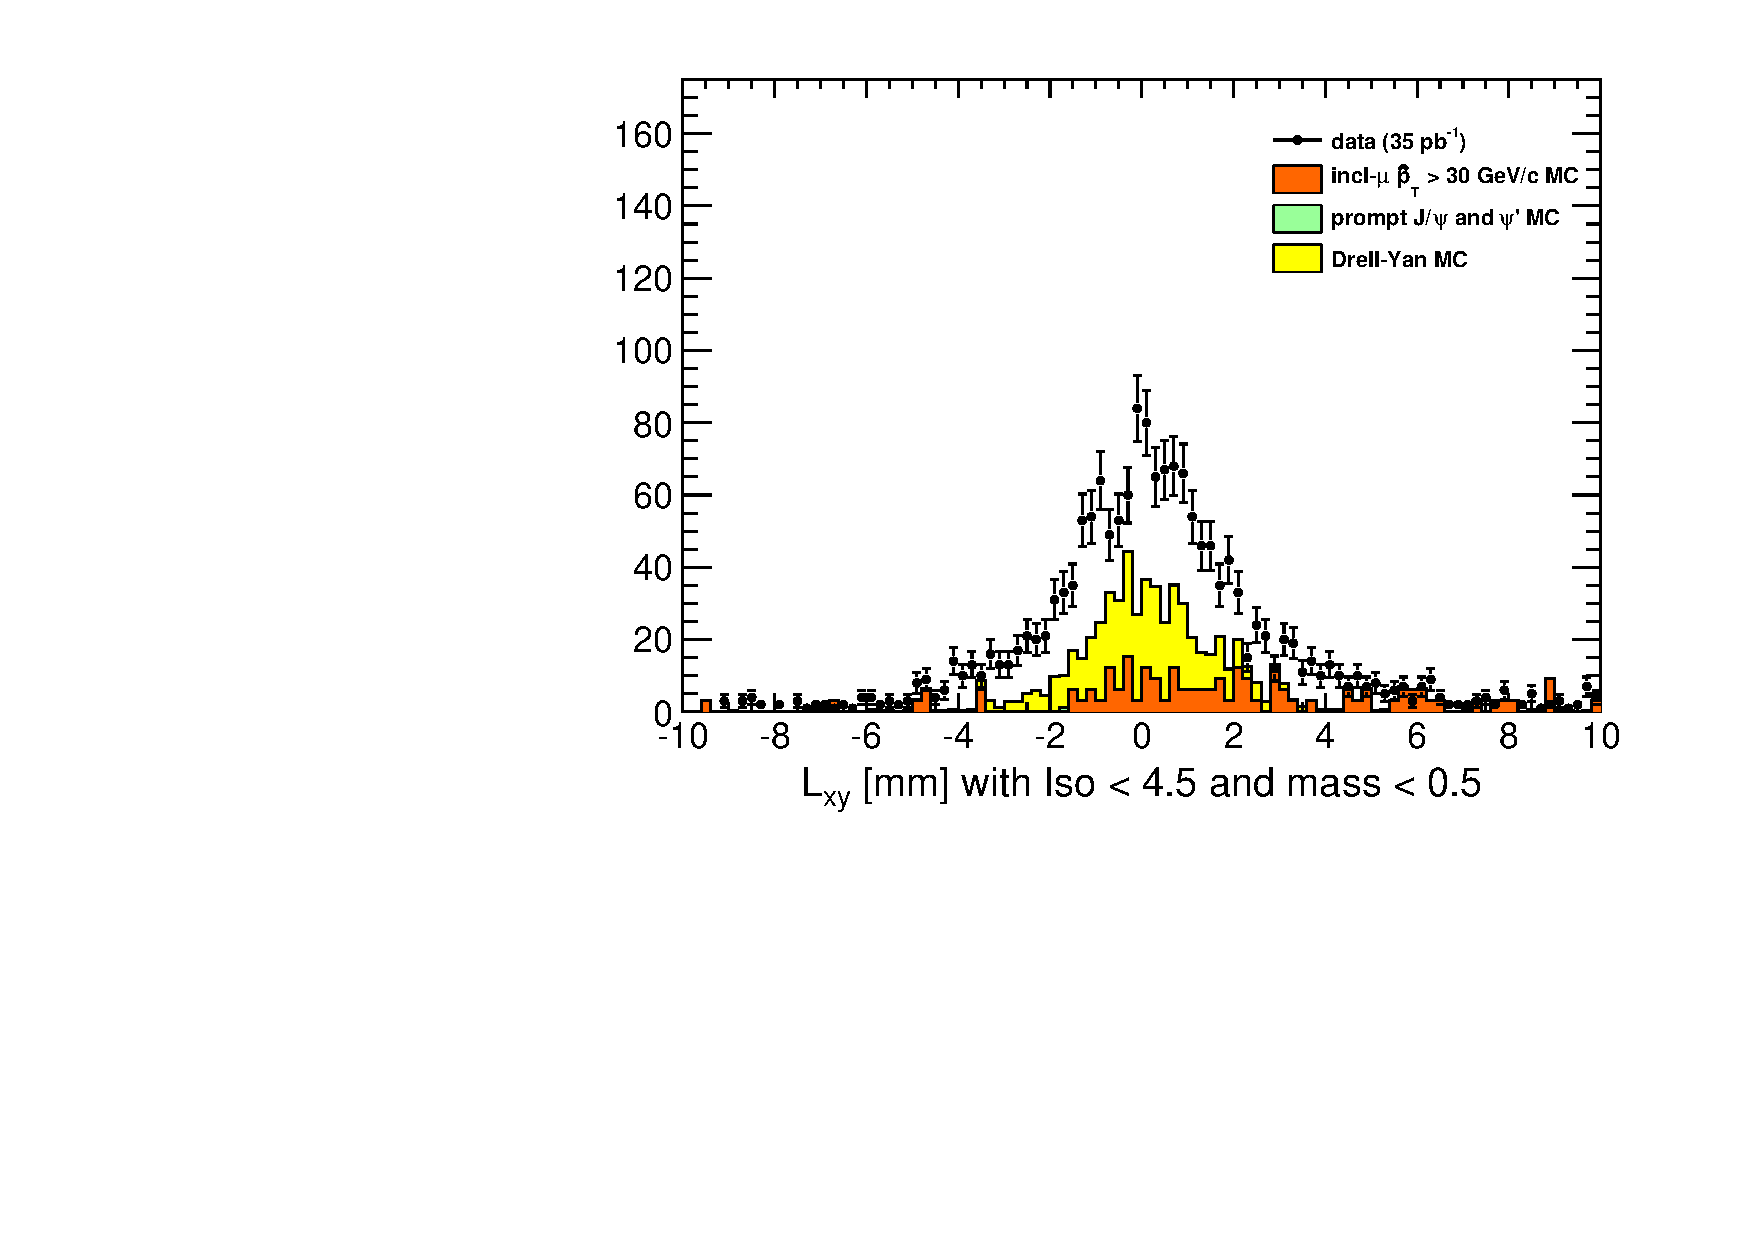
\includegraphics[width=1.2\linewidth]{lowdimuon_lxy_lowmass_isolated.pdf}

\column{0.5\linewidth}
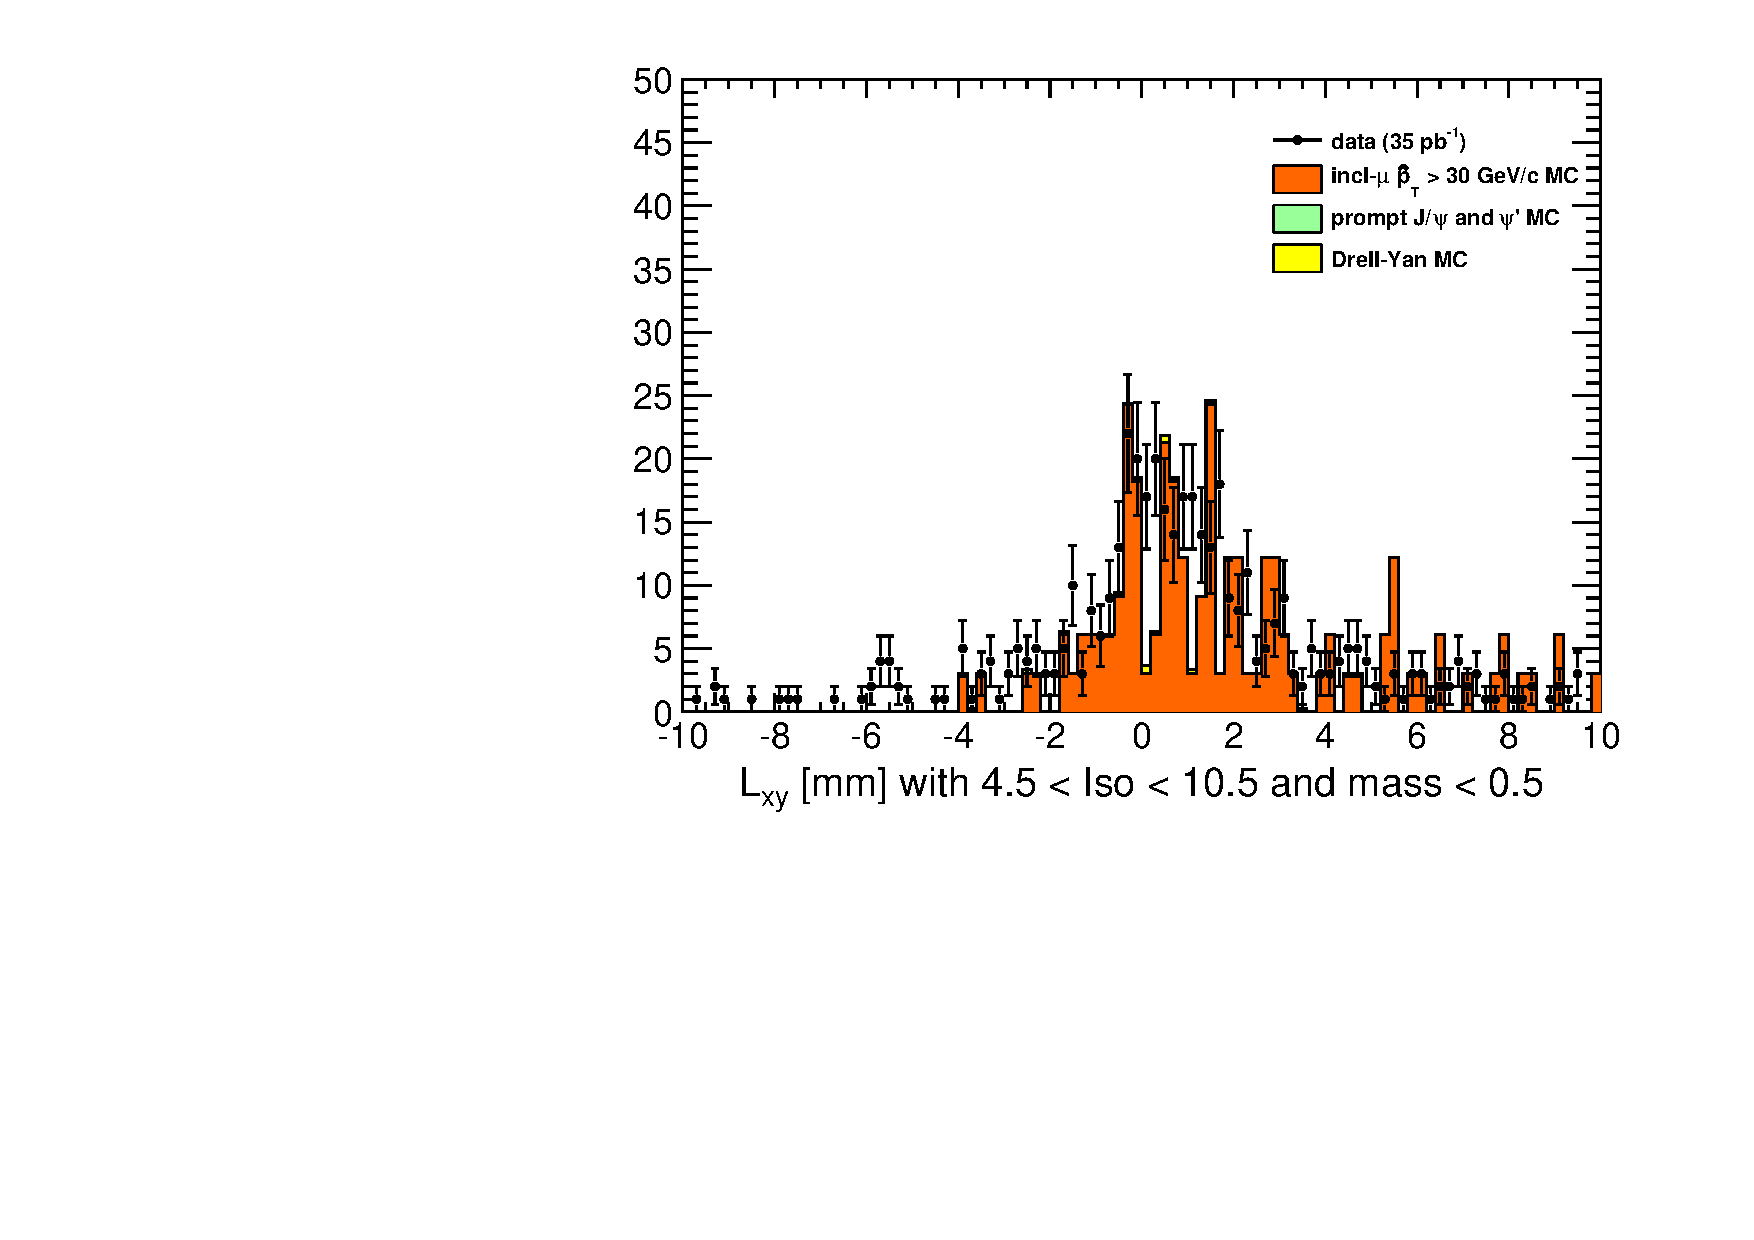
\includegraphics[width=\linewidth]{lowdimuon_lxy_lowmass_isosideband.pdf}

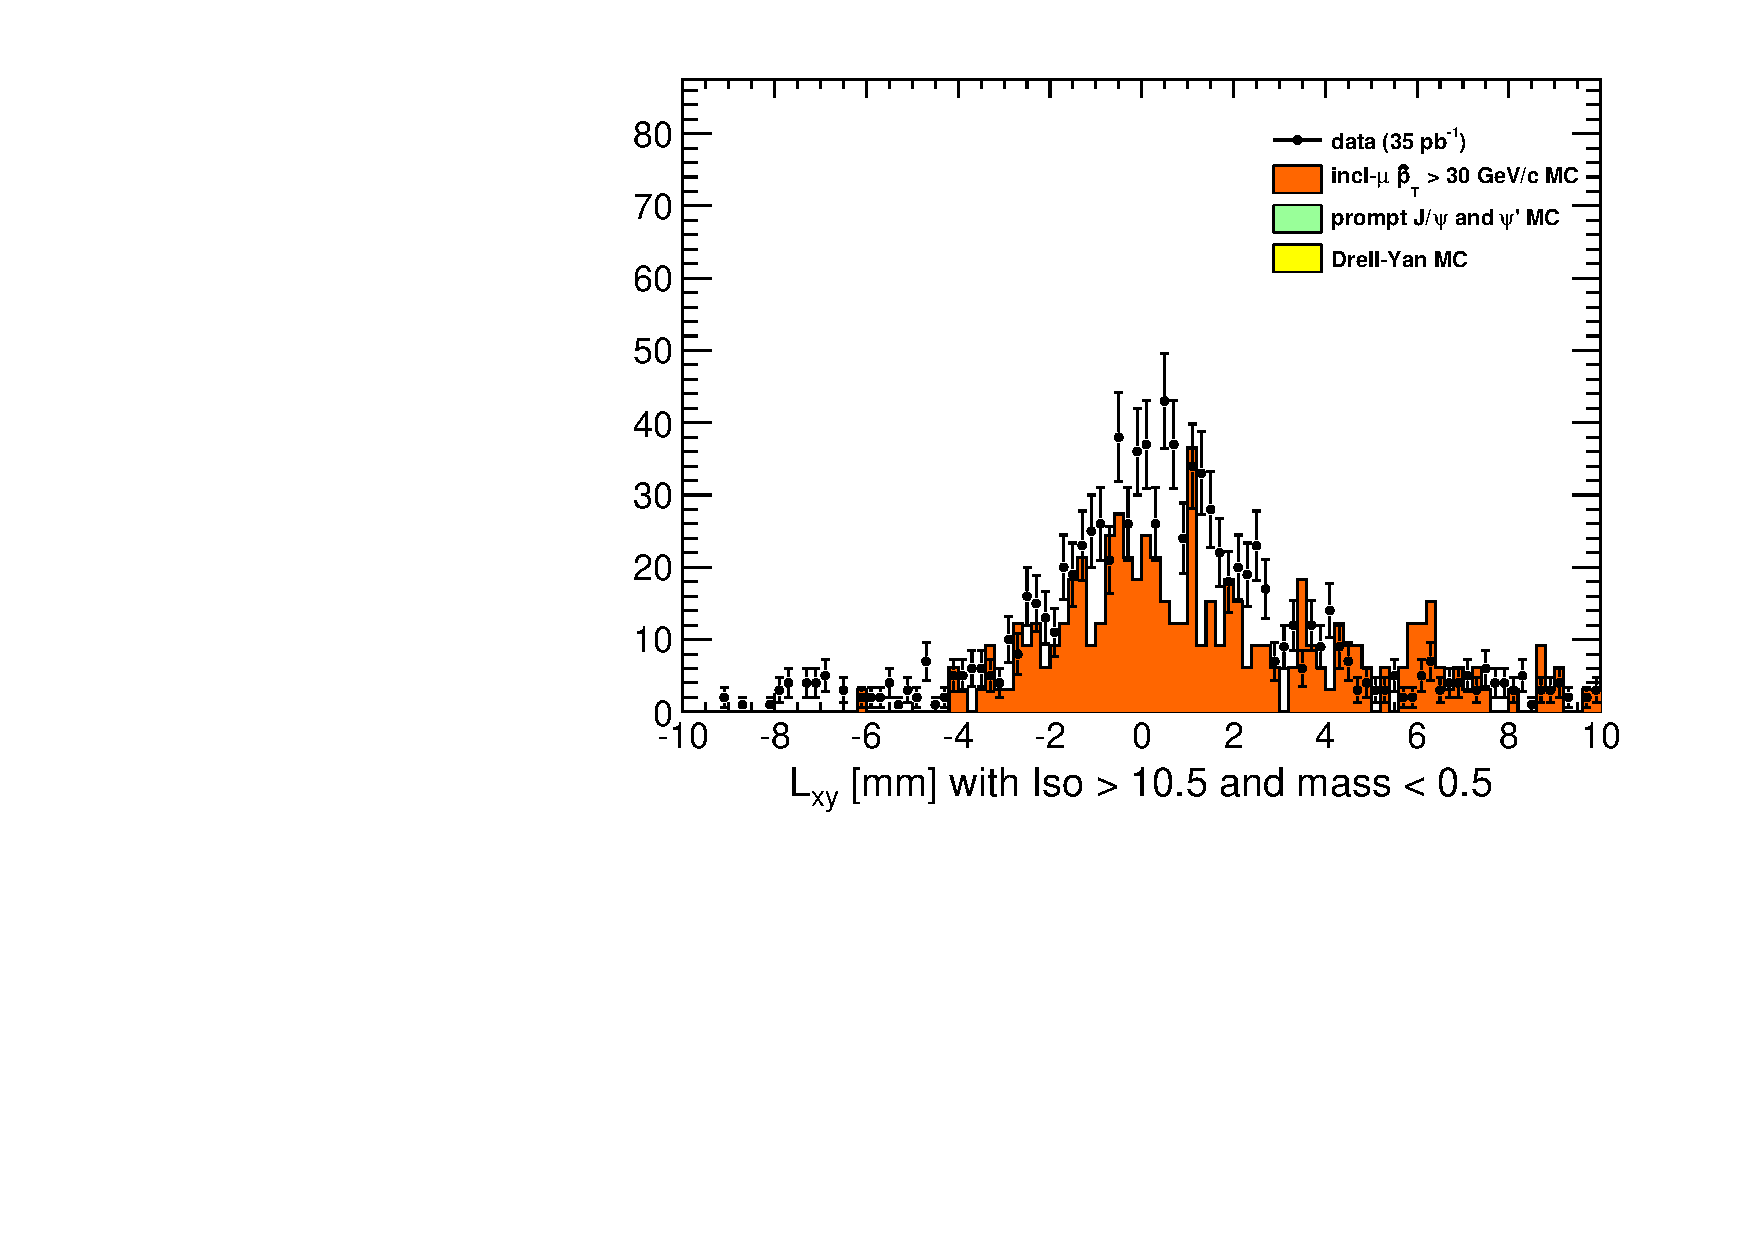
\includegraphics[width=\linewidth]{lowdimuon_lxy_lowmass_noniso.pdf}
\end{columns}
\end{frame}

\begin{frame}
\frametitle{Study of low-$p_T$ dimuon control}
\begin{itemize}
\item The low-mass dimuons are good muons (both the isolated and the
  non-isolated low-mass excesses)

\mbox{ } \hfill 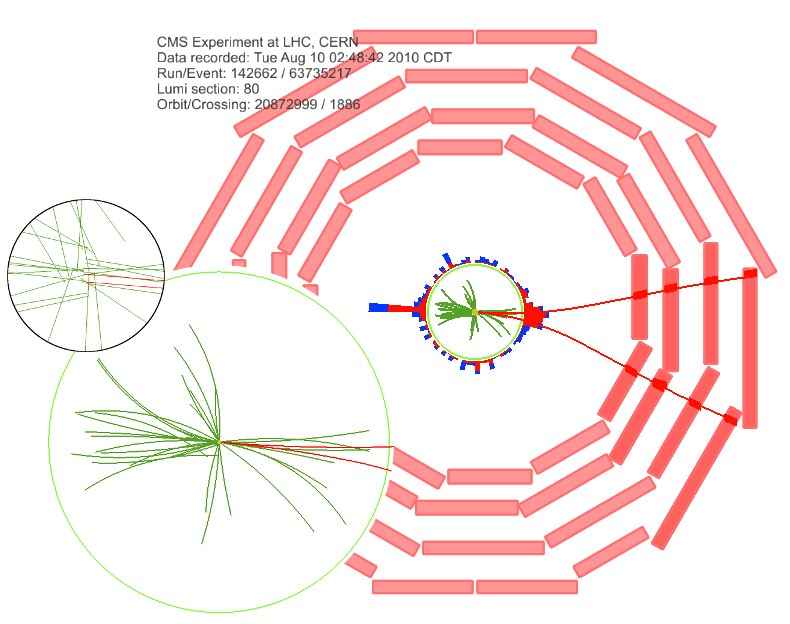
\includegraphics[width=0.8\linewidth]{lowmass_example.png} \hfill \mbox{ }

\item Also checked muon quality distributions (backup slides)
\end{itemize}
\end{frame}

\begin{frame}
\frametitle{Study of low-$p_T$ dimuon control}
\begin{itemize}
\item Tentative conclusions (gathered onto one slide):
\begin{itemize}
\item continuous $Iso < 4.5$~GeV/$c$, $1.1 < \mbox{mass} < 2.9$~GeV/$c^2$ data-excess is likely the $\hat{p}_T < 30$~GeV/$c$ part of the inclusive-muon
\begin{itemize}
\item simply wasn't generated (it's CPU-intensive in Pythia)
\item regions dominated by high-$\hat{p}_T$ match perfectly
\item ppMuX (no $\hat{p}_T$ cut) has this continuous shape
\end{itemize}
\item narrow data-excess in mass $<$ 0.5~GeV/$c^2$:
\begin{itemize}
\item is {\it not} due to fake muons
\item is too wide to be a resonance, but has an endpoint at the $\eta$ mass, so $\eta \to \mu\mu\gamma$ is possible ($\mathcal{B}(\eta \to \mu\mu\gamma) = 3\times 10^{-4}$, $\mathcal{B}(\eta \to \mu\mu) = 6\times 10^{-6}$, similar to $\mathcal{B}(\omega, \phi \to \mu\mu) \sim 10^{-4}$)
\item the isolated part could be partially Drell-Yan (normalization from the $Z$ may not be correct when scaled down to zero mass)
\item but a significant part of it is non-isolated ($\eta$ produced in $b$-jets?  Could be hard to find the $\gamma$ inside jets)
\end{itemize}
\end{itemize}

\item Currently using only $0.3 < mass < 5$~GeV/$c^2$ part of the
  spectrum; could push lower, depending on level of confidence with
  these incompletely understood events
\end{itemize}
\end{frame}

\begin{frame}
\frametitle{Deriving a mass template}

\begin{itemize}
\item The control region contains $b\bar{b}$, Drell-Yan, and prompt resonances
\item Backgrounds in the dimuon-dimuon signal region
  \textcolor{darkblue}{(b-1)} are dominated by $b\bar{b}$, because
  each $b$-quark can produce two nearby muons and there are two
  $b$-quarks in $b\bar{b}$ events (other processes would require
  coincidences to produce four muons)
\item To reject Drell-Yan and prompt resonances, select

\mbox{ } \hfill $Iso > 4.5$~GeV/$c$ {\bf or} $L_{xy} > 2$~mm \hfill \mbox{ }

\item Selection is loose, purifies $b\bar{b}$ (including resonances in
  $b\bar{b}$), and has a constant efficiency across the mass spectrum: this is the template
\end{itemize}

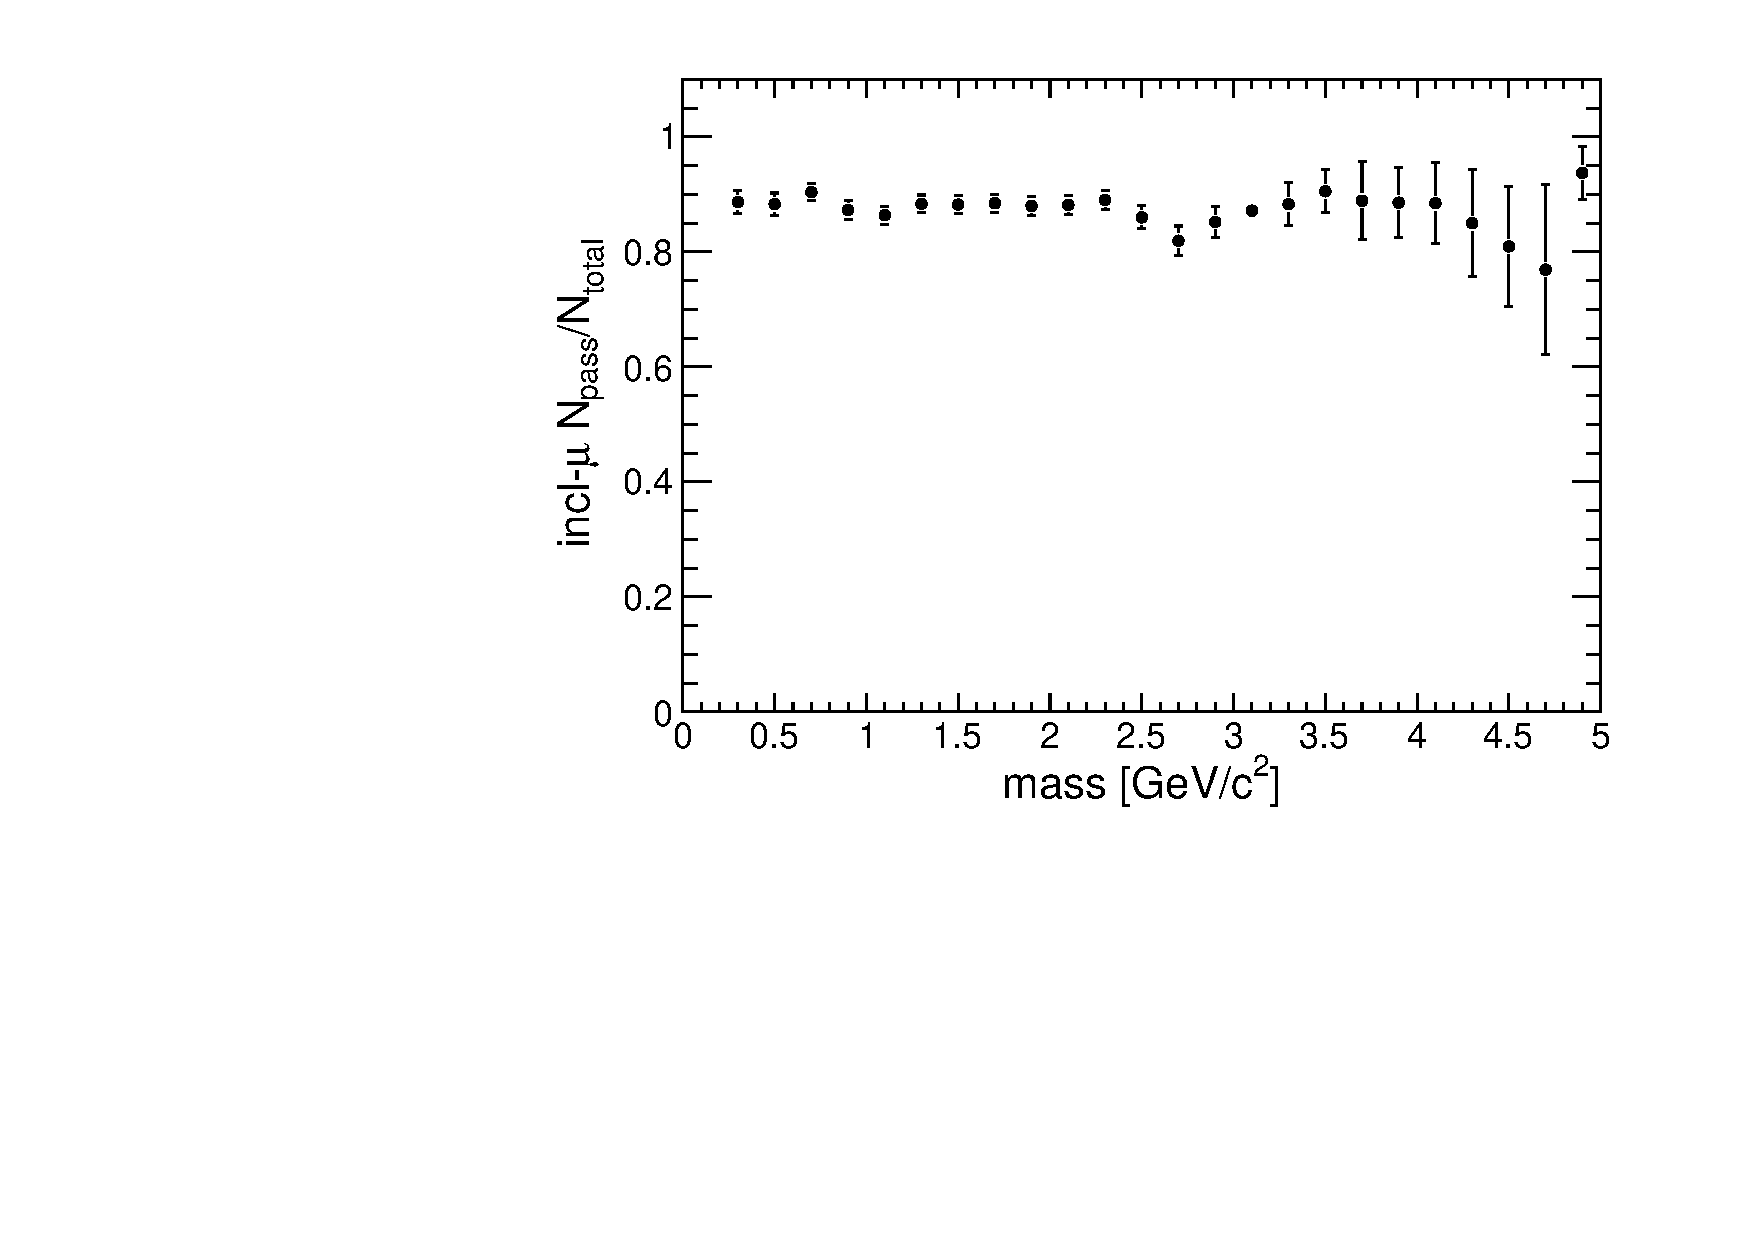
\includegraphics[width=0.5\linewidth]{lowdimuon_mass_bcut_efficiency.pdf}
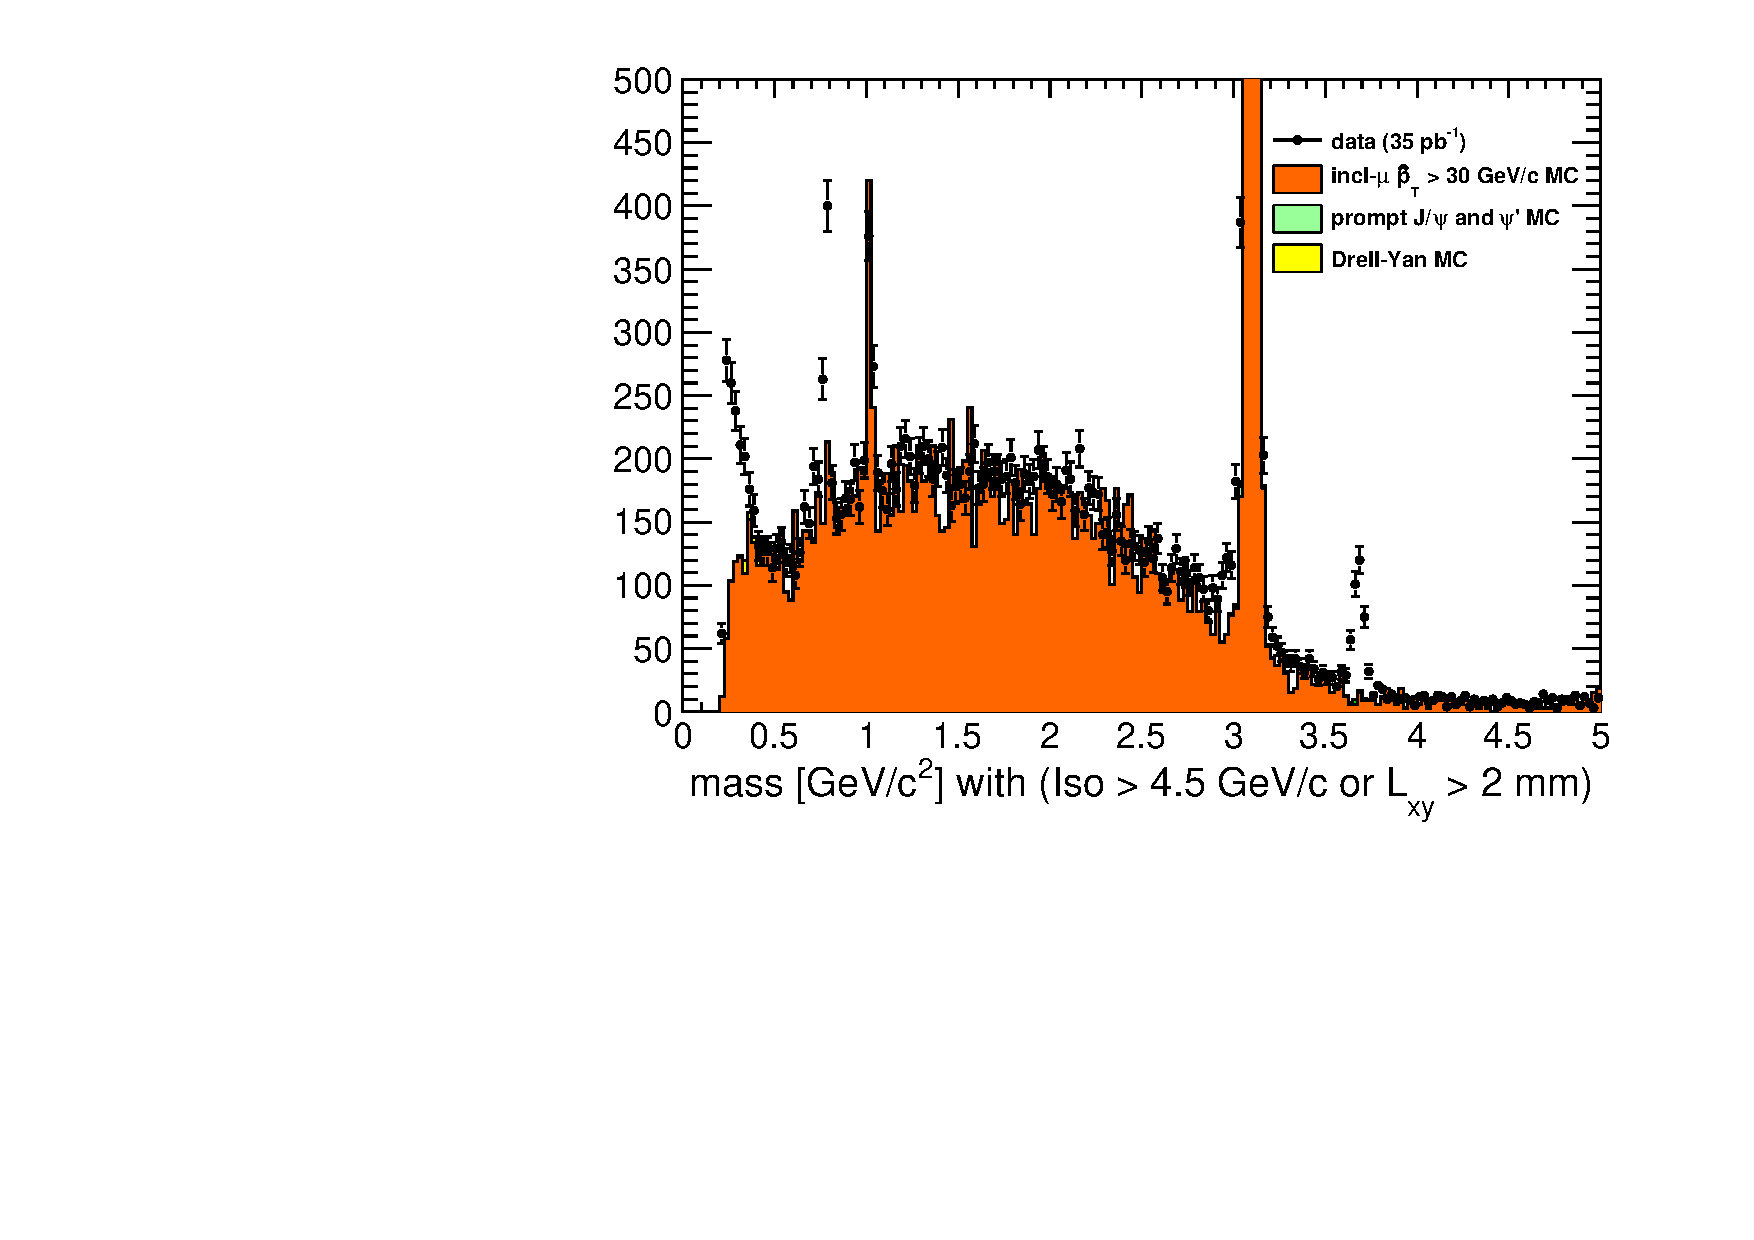
\includegraphics[width=0.5\linewidth]{lowdimuon_mass_bcuts.pdf}
\end{frame}

\begin{frame}
\frametitle{Parameterized mass templates}

\begin{columns}
\column{0.35\linewidth}
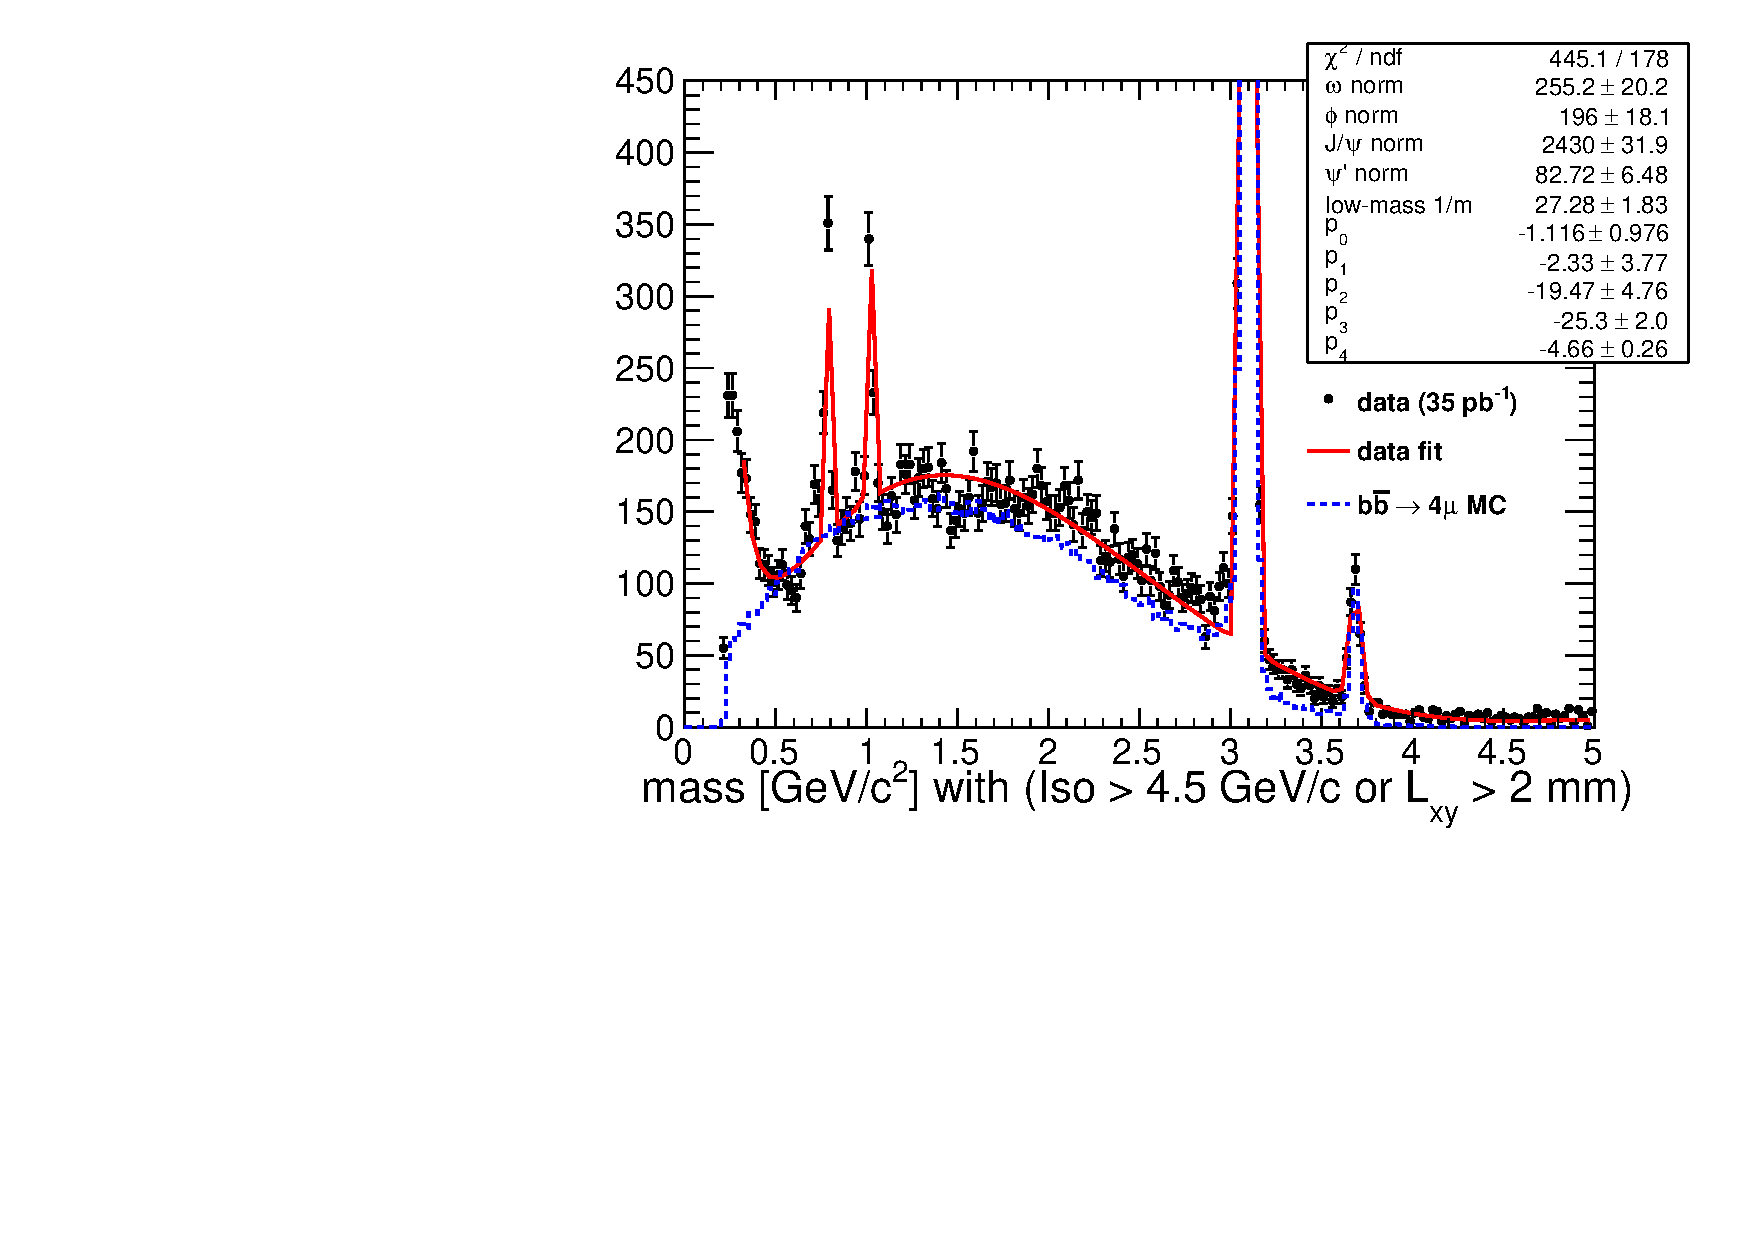
\includegraphics[width=\linewidth]{lowdimuon_mass_bcuts_backgroundfit_zoom.pdf}

\column{0.65\linewidth}
\textcolor{darkblue}{Purpose:} in the dimuon-dimuon channel \textcolor{darkblue}{(b-1)}, this is for the dimuon that contains a high-$p_T$ barrel muon to satisfy the trigger

\textcolor{darkblue}{Derived from:} $b\bar{b}$-enriched low-$p_T$ dimuon control sample (previous page)
\end{columns}

\begin{columns}
\column{0.35\linewidth}
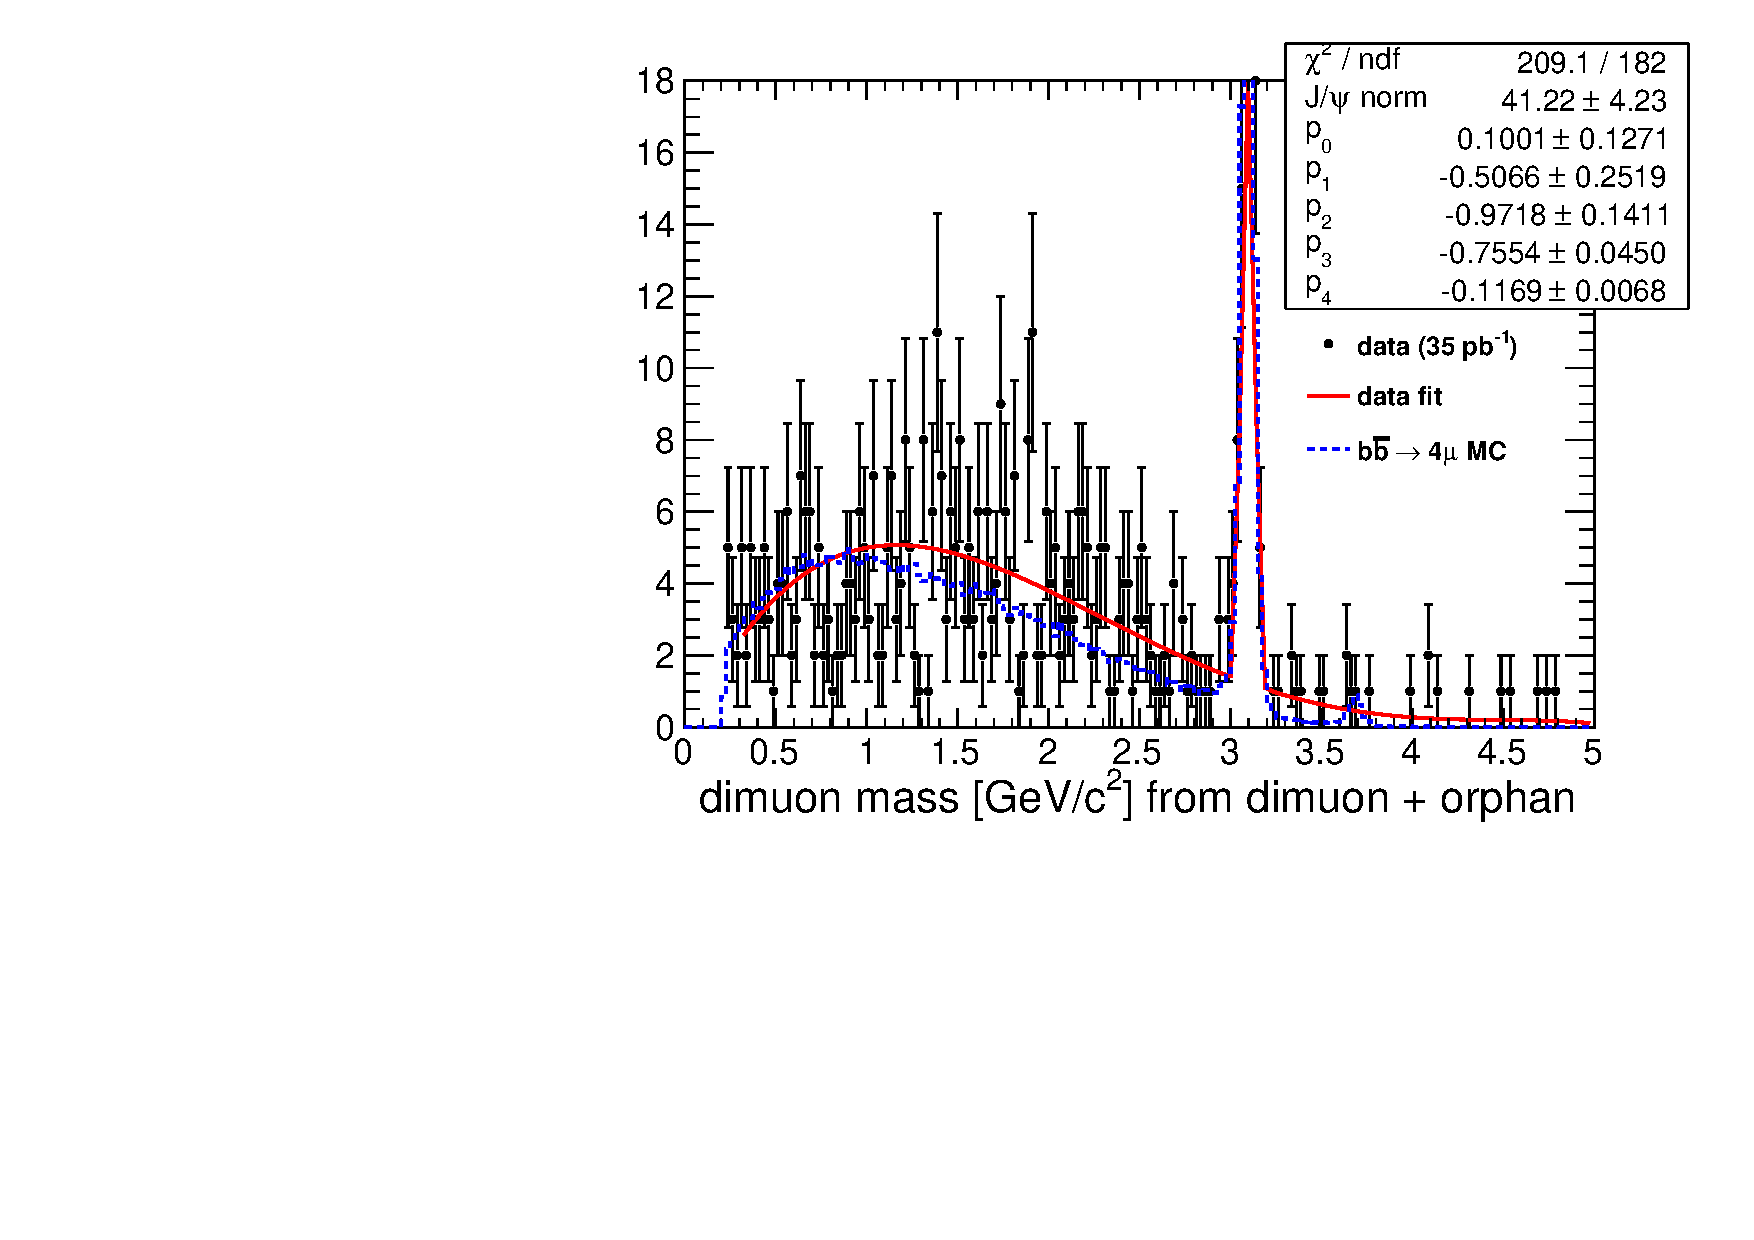
\includegraphics[width=\linewidth]{dimuorphan_mass_fit_zoom.pdf}

\column{0.65\linewidth}
\textcolor{darkblue}{Purpose:} in the dimuon-dimuon channel \textcolor{darkblue}{(b-1)}, this is for the other dimuon

\textcolor{darkblue}{Derived from:} dimuon + orphaned muon control sample, where the orphaned muon was selected to satisfy the trigger
\end{columns}

\begin{columns}
\column{0.35\linewidth}
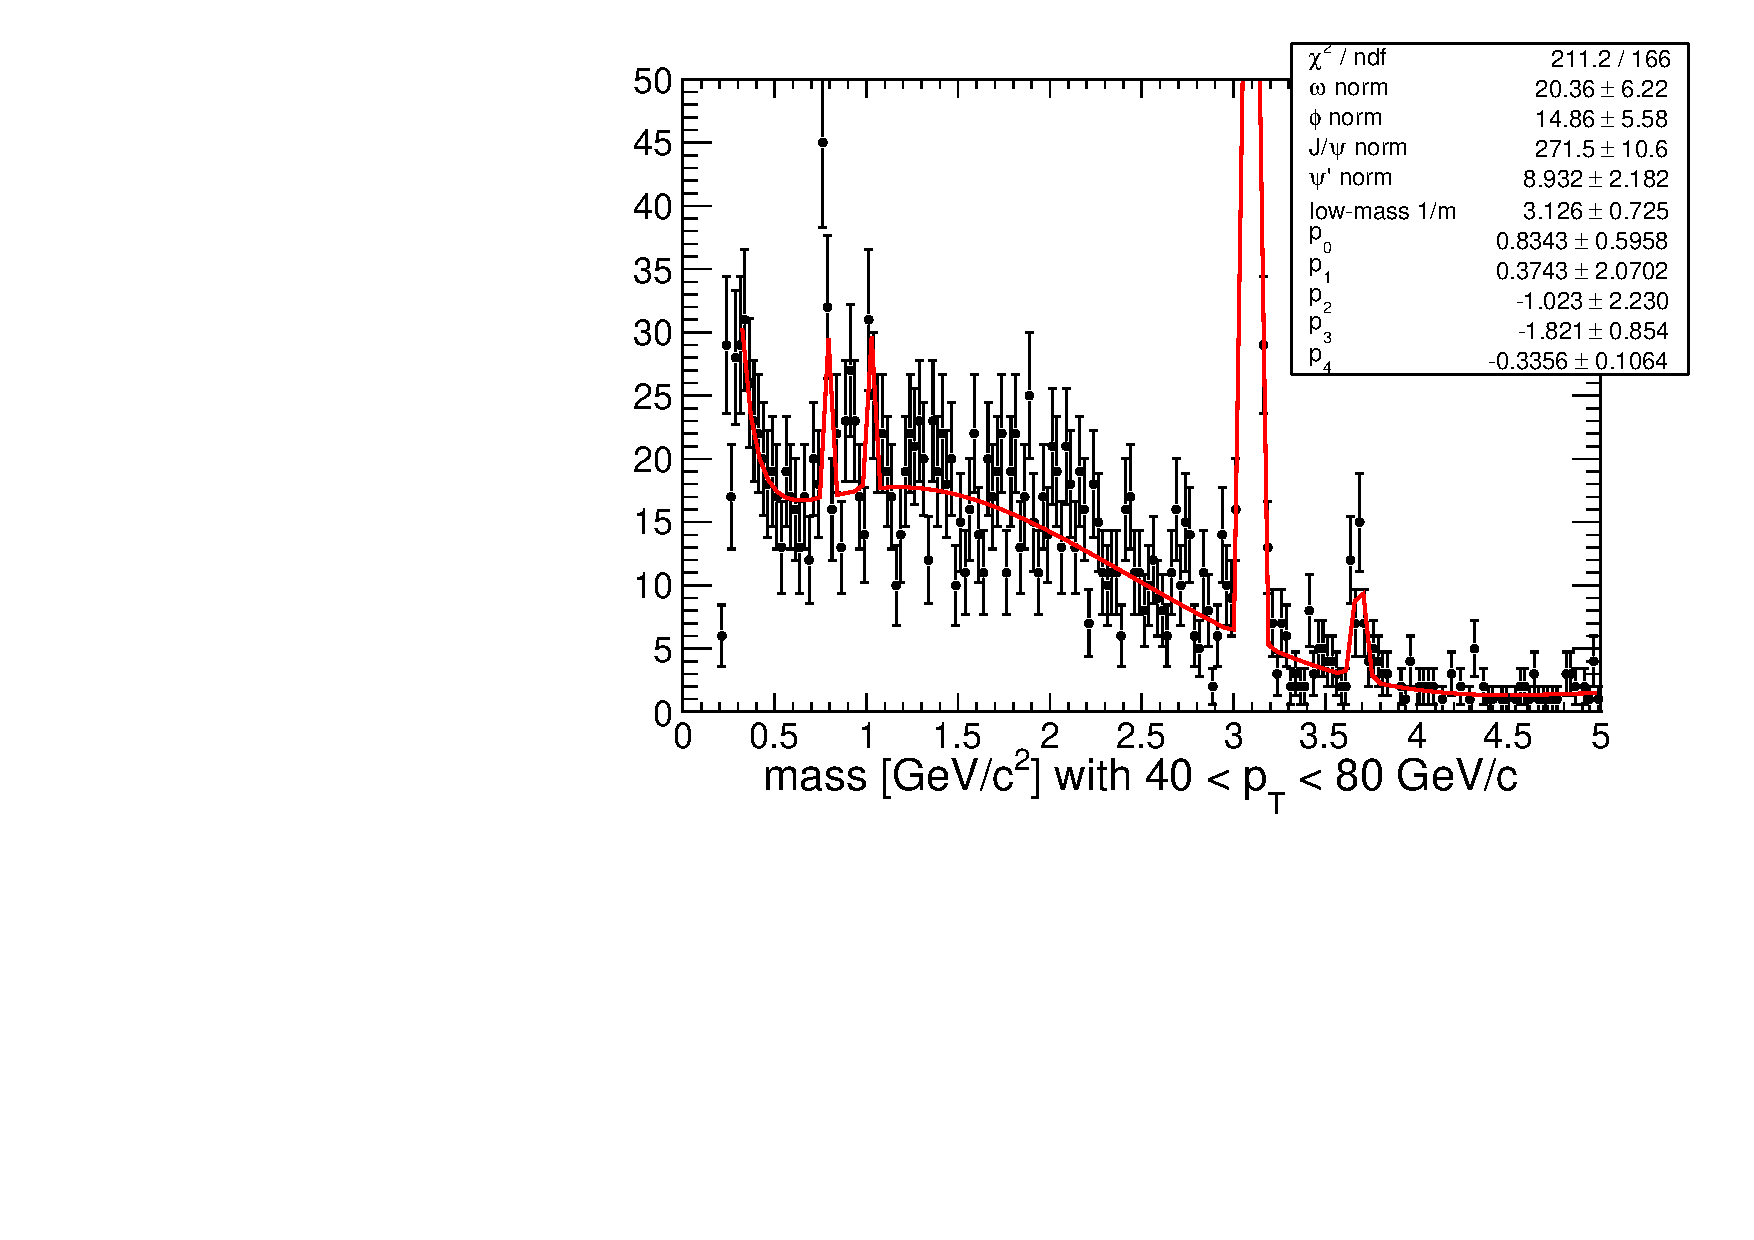
\includegraphics[width=\linewidth]{lowdimuon_40-80_backgroundfit_zoom.pdf}

\column{0.65\linewidth}
\textcolor{darkblue}{Purpose:} this is for the $p_T > 80$~GeV/$c$ dimuon channel \textcolor{darkblue}{(a-1)}

\textcolor{darkblue}{Derived from:} all events ($b\bar{b}$, Drell-Yan, prompt) in $40 < p_T < 80$~GeV/$c$, since their ratio is constant above 40~GeV/$c$
\end{columns}

Similarly, templates for ``4 muons in one mu-jet'' \textcolor{darkblue}{(a-2, b-2, b-3)} will be derived from ``2 muons + 2 tracks'' control sample
\end{frame}

\begin{frame}
\frametitle{Sample fitter output}

\begin{columns}
\column{0.5\linewidth}
\begin{itemize}
\item A fitter originally for the NMSSM case is being generalized
  to $N$-dimuon mass fits and ported to RooFit

\item Top-right: a 1-dimuon fit with data-driven backgrounds template,
  fake 2~GeV/$c^2$ signal, and simulated data
\begin{itemize}
\item 20 signal events, 100 background events
\end{itemize}

\item Bottom-right: upper limits on yield
  as a function of $m_1$ mass
\end{itemize}

\column{0.5\linewidth}
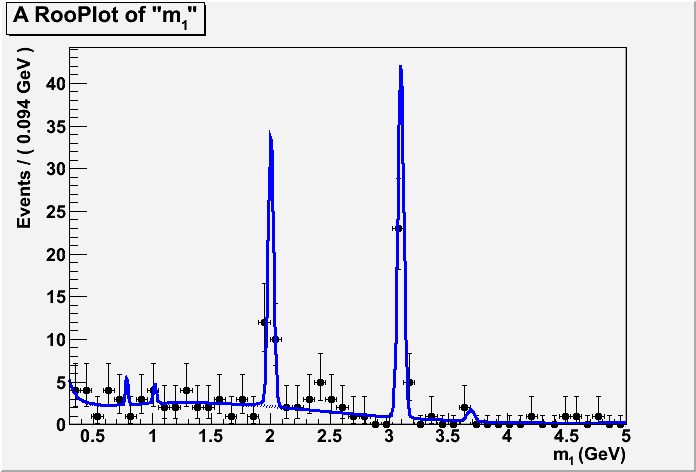
\includegraphics[width=\linewidth]{model_s20b100.png}

\vspace{0.5 cm}
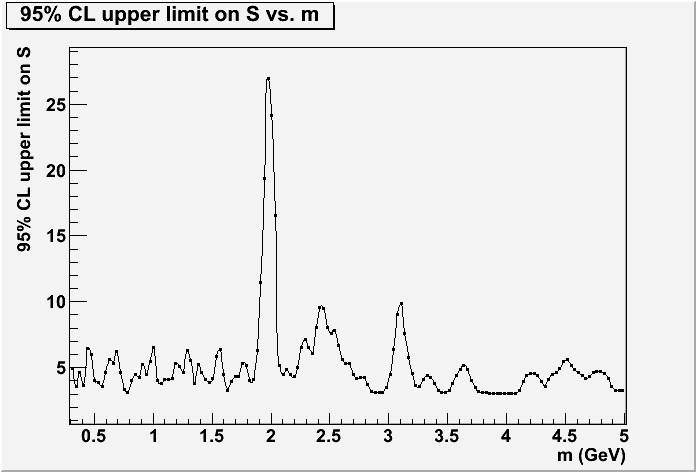
\includegraphics[width=\linewidth]{ul_s20b100_likelihood.png}
\end{columns}
\end{frame}

\begin{frame}
\frametitle{2-D mass template}

\begin{itemize}
\item Since the two $b$-quarks decay or attach fake muons to
  themselves independently, we construct a mass template by a
  Cartesian product
\item We can cross-check the shape of both distributions with the
  slices that include the $J/\psi$:
\begin{center}
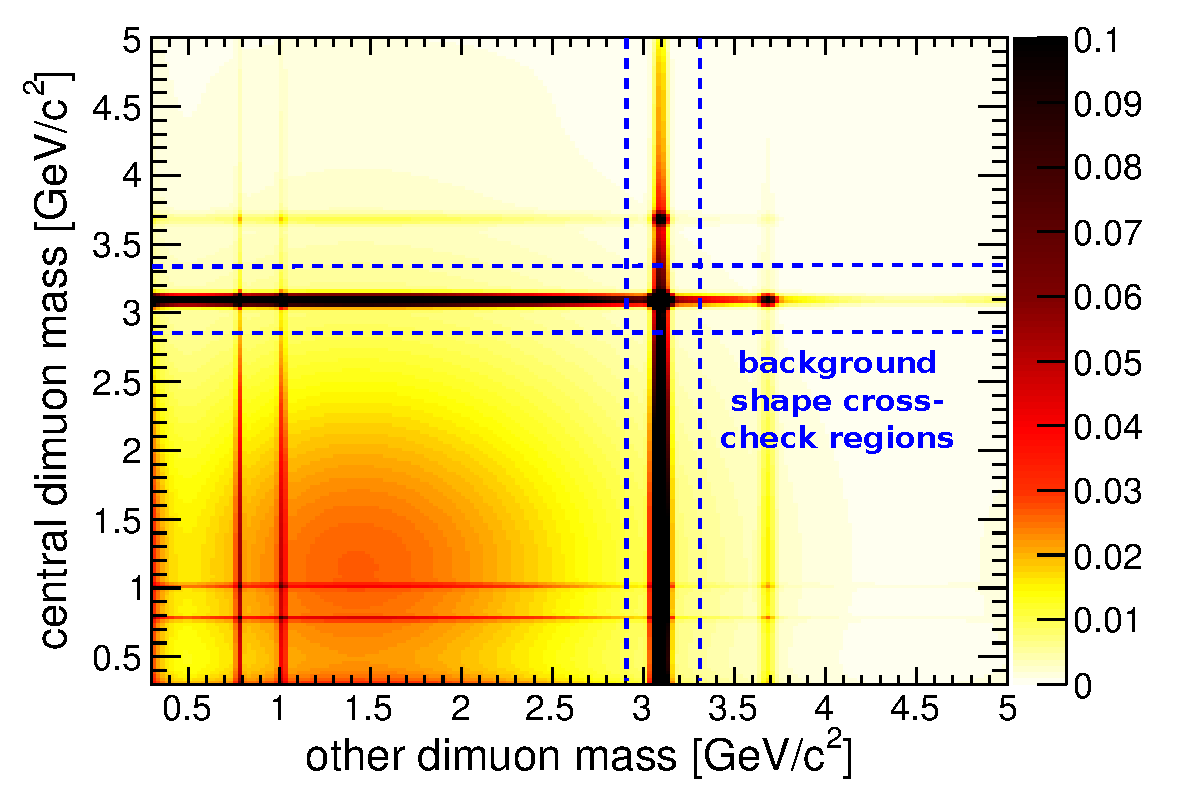
\includegraphics[width=0.9\linewidth]{background_2d_mass_template.pdf}
\end{center}
\end{itemize}
\end{frame}

\begin{frame}
\frametitle{Mass resolution}

\begin{itemize}
\item Hidden sector bosons have negligible intrinsic width, so we can
  determine the width of the signal peak from our four narrow Standard
  Model resonances: $\omega$, $\phi$, $J/\psi$, and $\psi'$
\end{itemize}

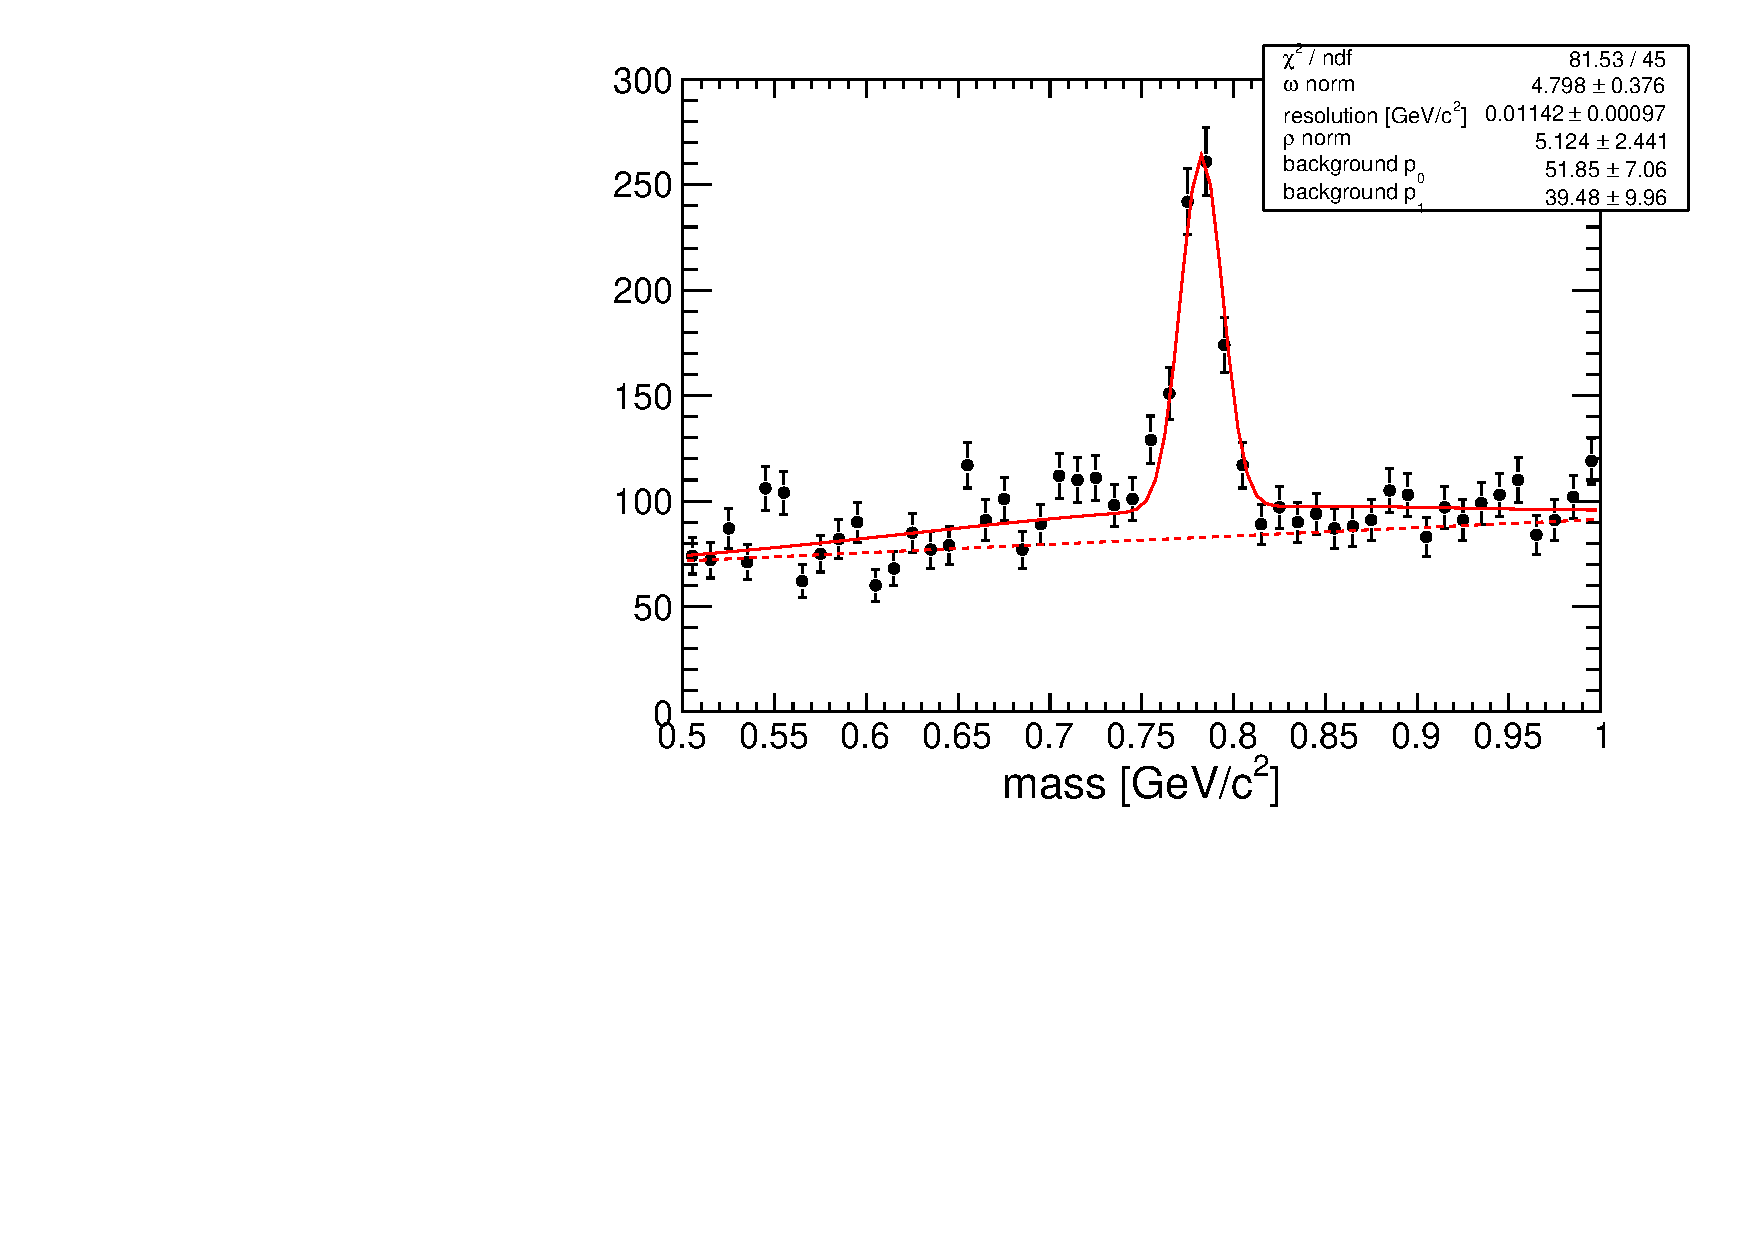
\includegraphics[width=0.47\linewidth]{respeak_omega.pdf}
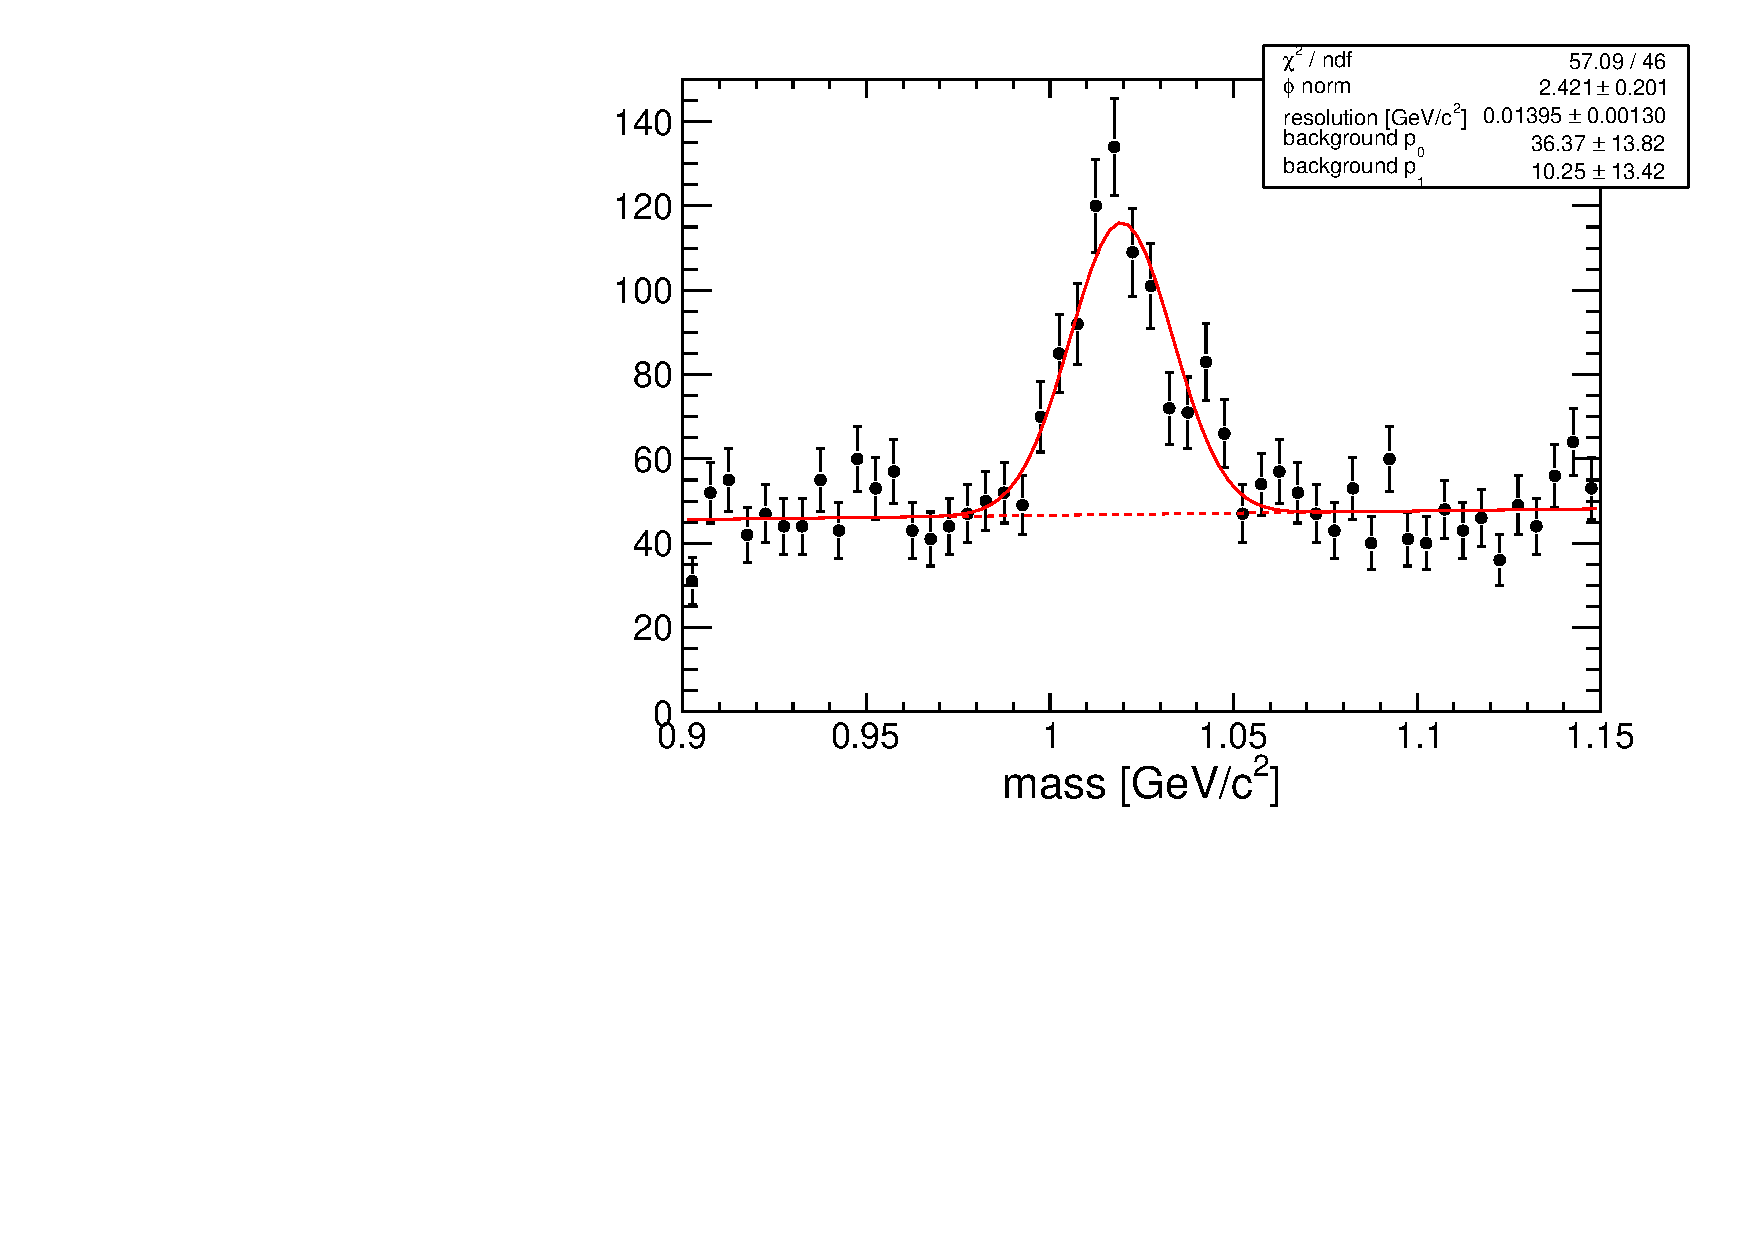
\includegraphics[width=0.47\linewidth]{respeak_phi.pdf}

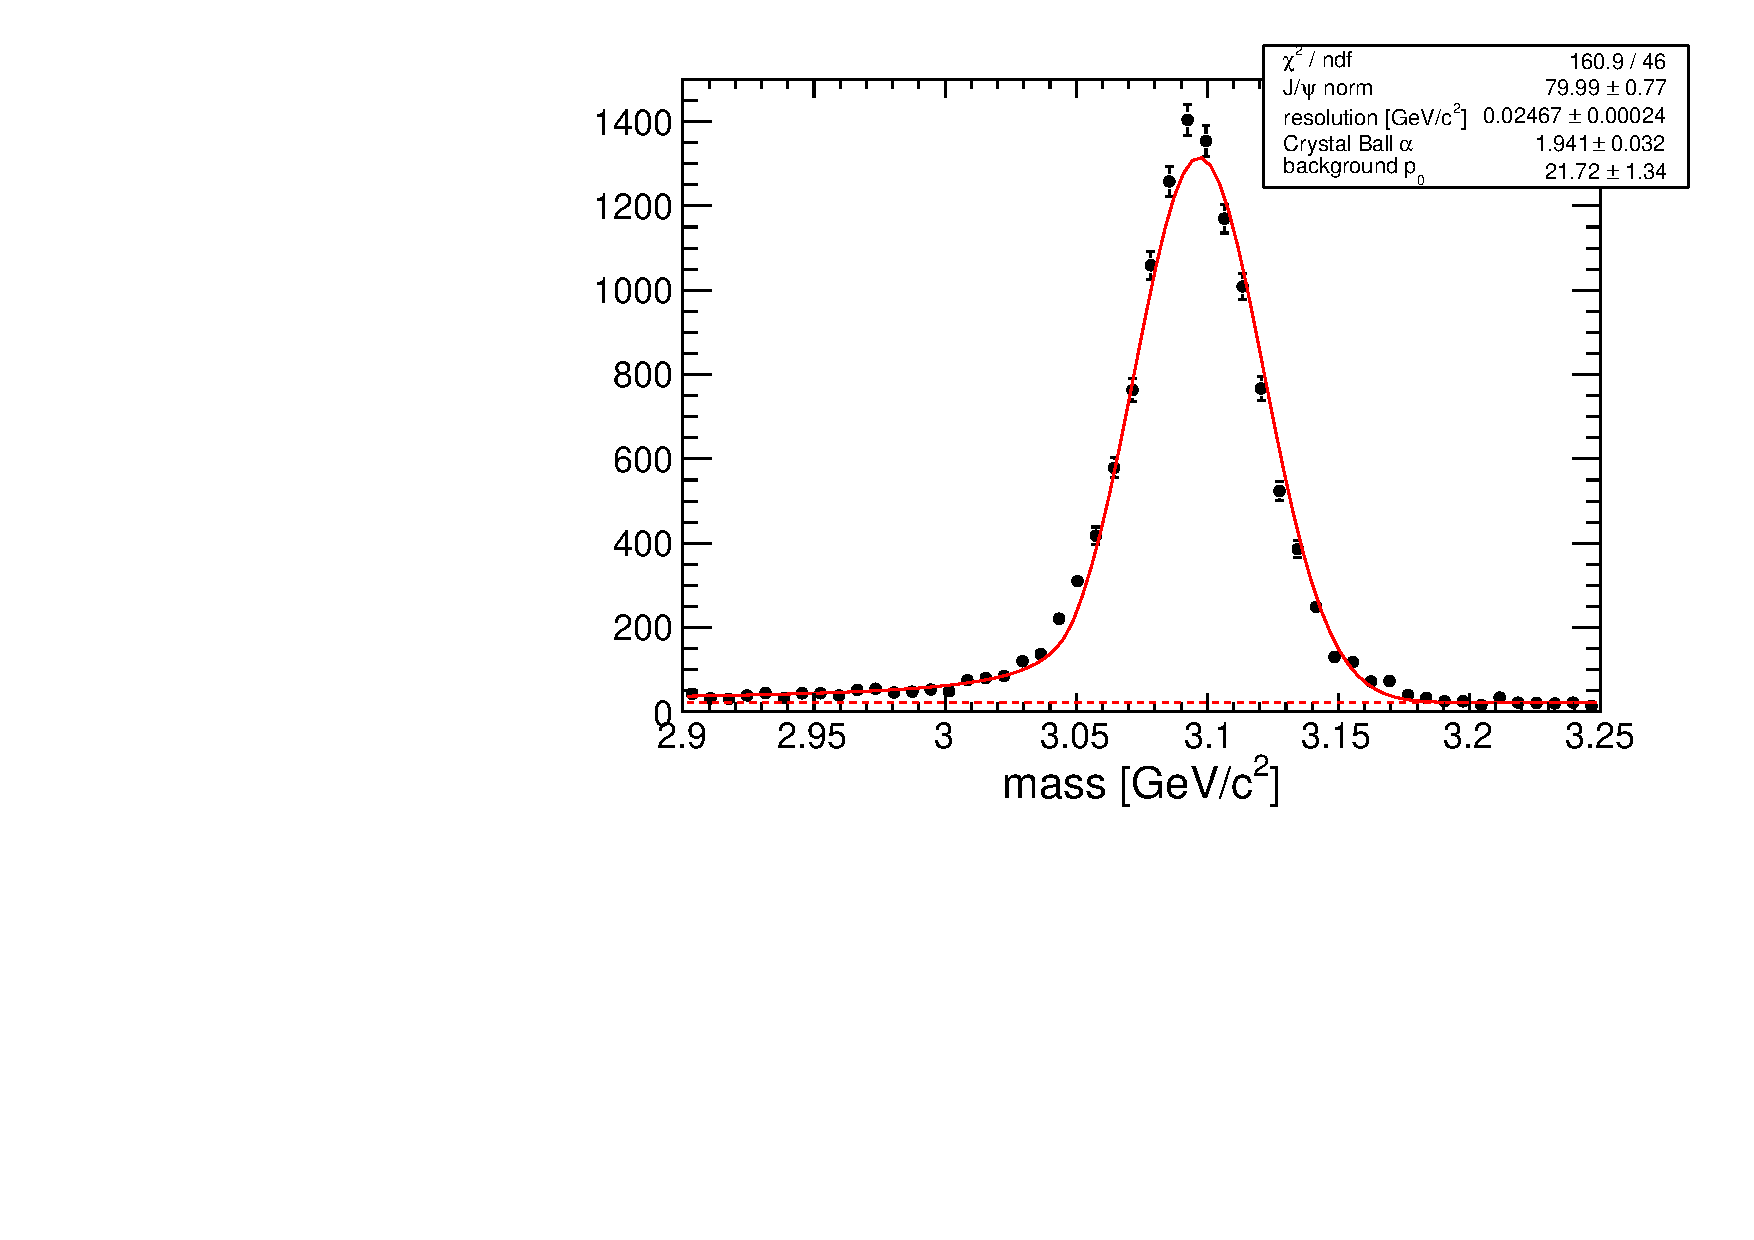
\includegraphics[width=0.47\linewidth]{respeak_jpsi.pdf}
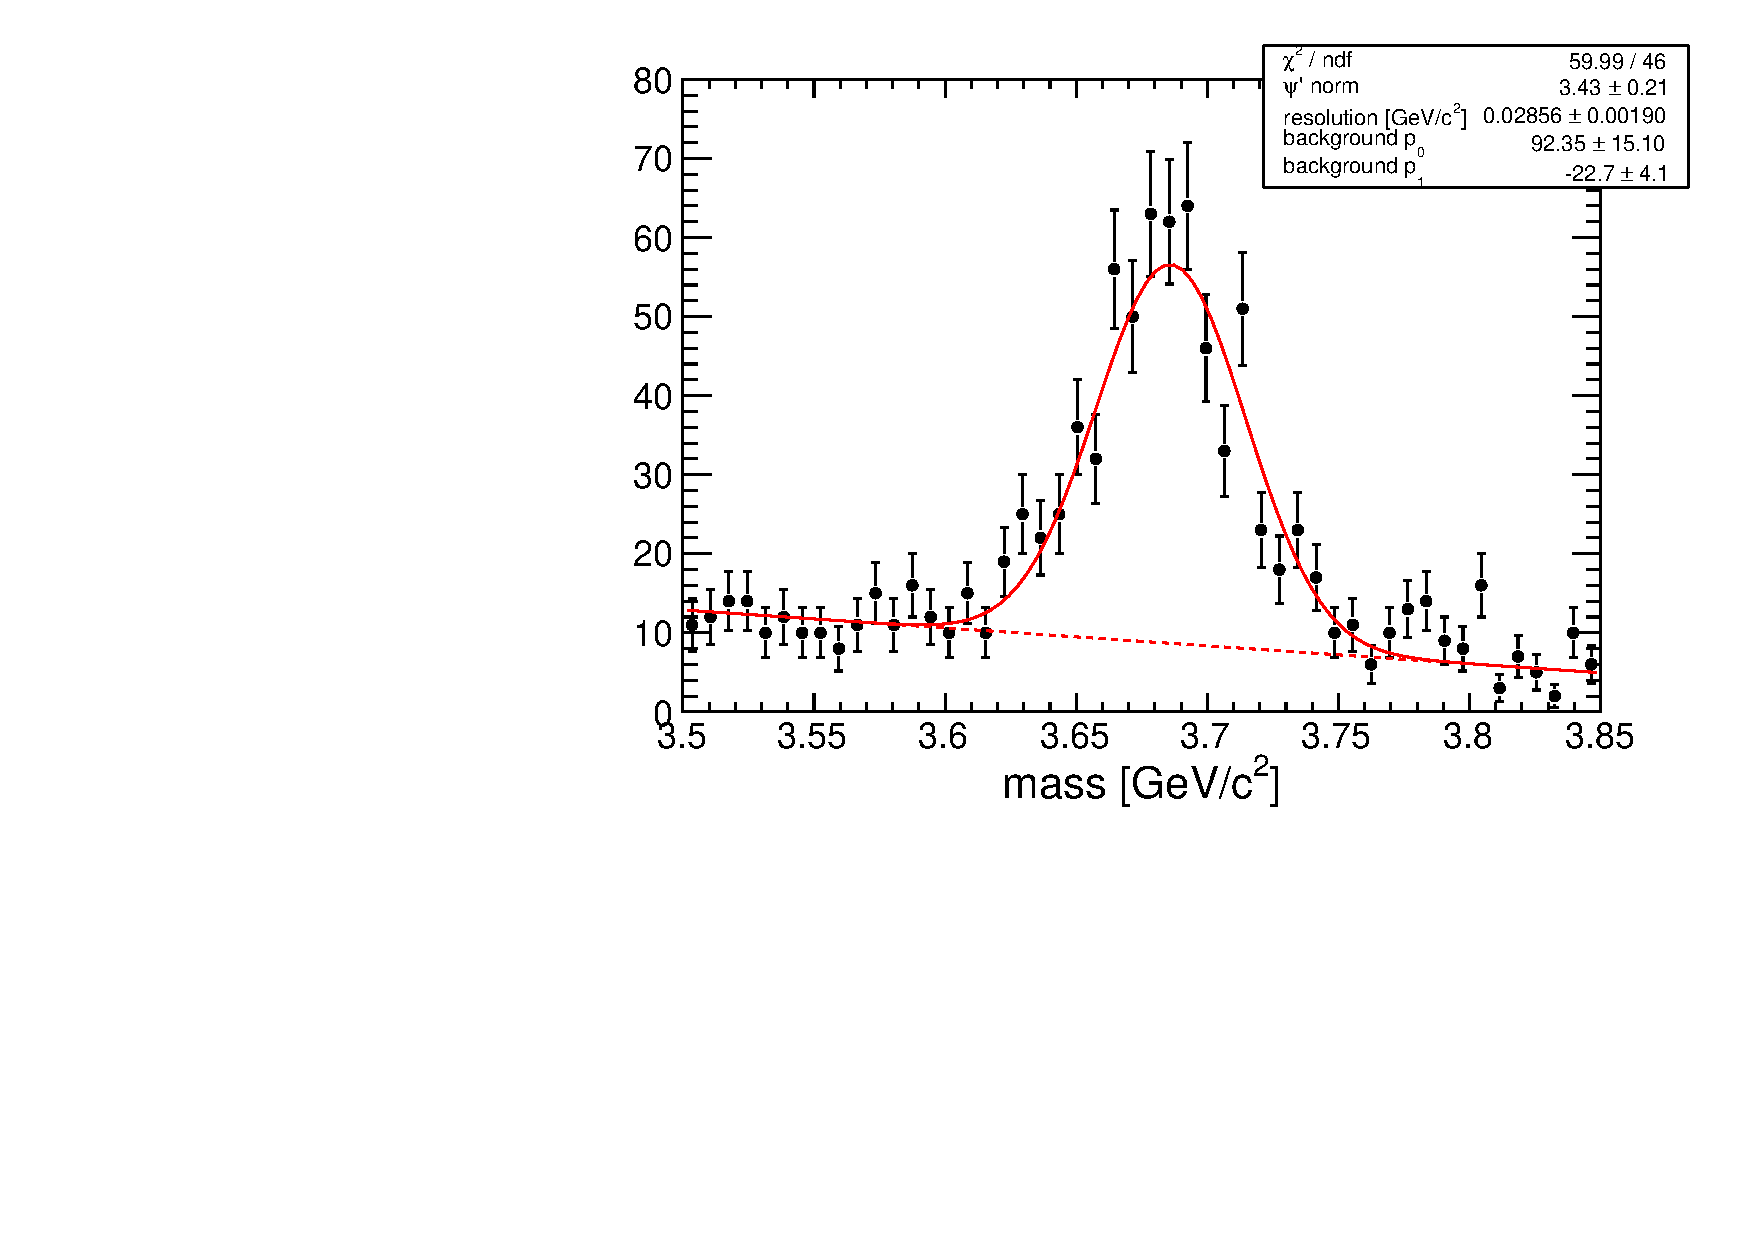
\includegraphics[width=0.47\linewidth]{respeak_psiprime.pdf}
\end{frame}

\begin{frame}
\frametitle{Mass resolution}

\begin{itemize}
\item The low-$p_T$ Standard Model resonances don't necessarily
  represent resolution for high-$p_T$ new physics, so check with a
  dimuon gun MC

\item Most of the difference is barrel vs.\ endcap, with only a weak
  dependence on momentum

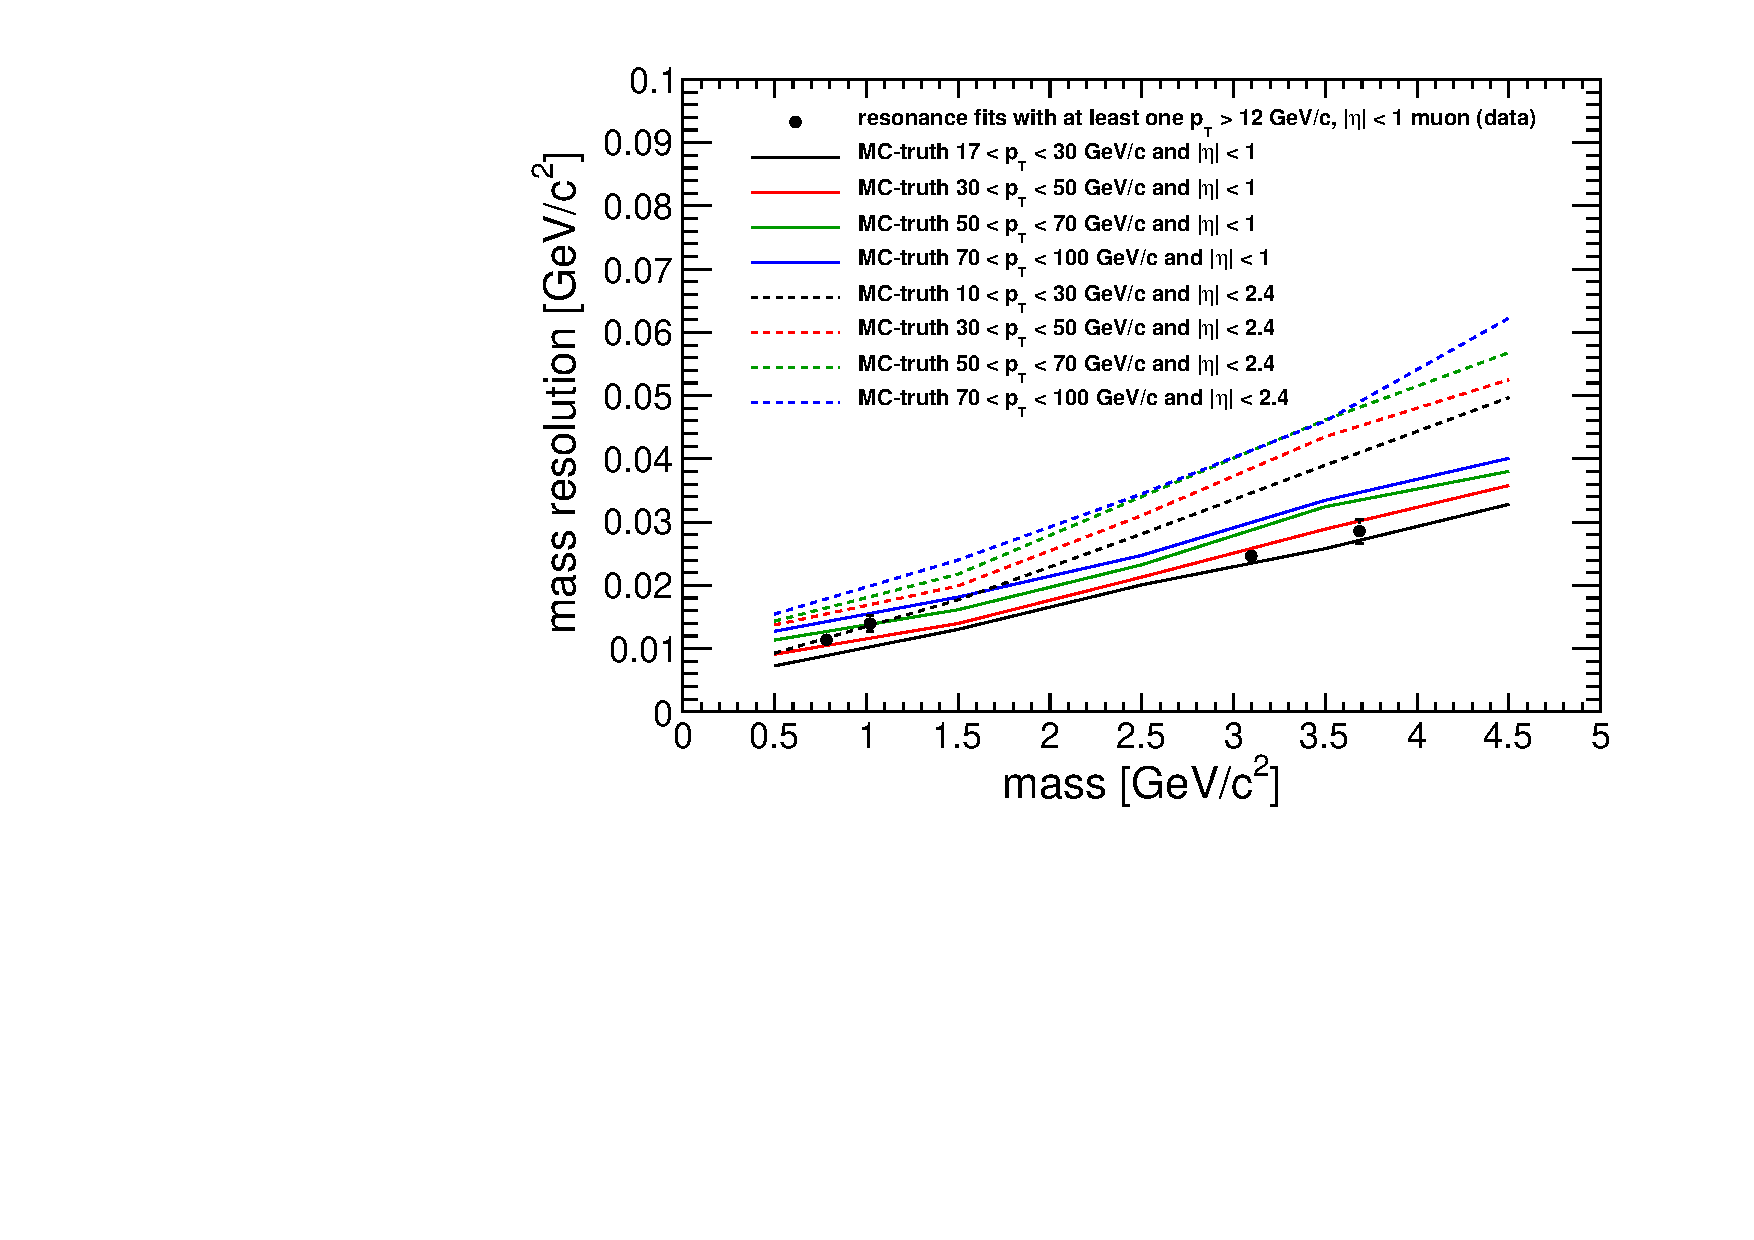
\includegraphics[width=0.5\linewidth]{resolution.pdf}
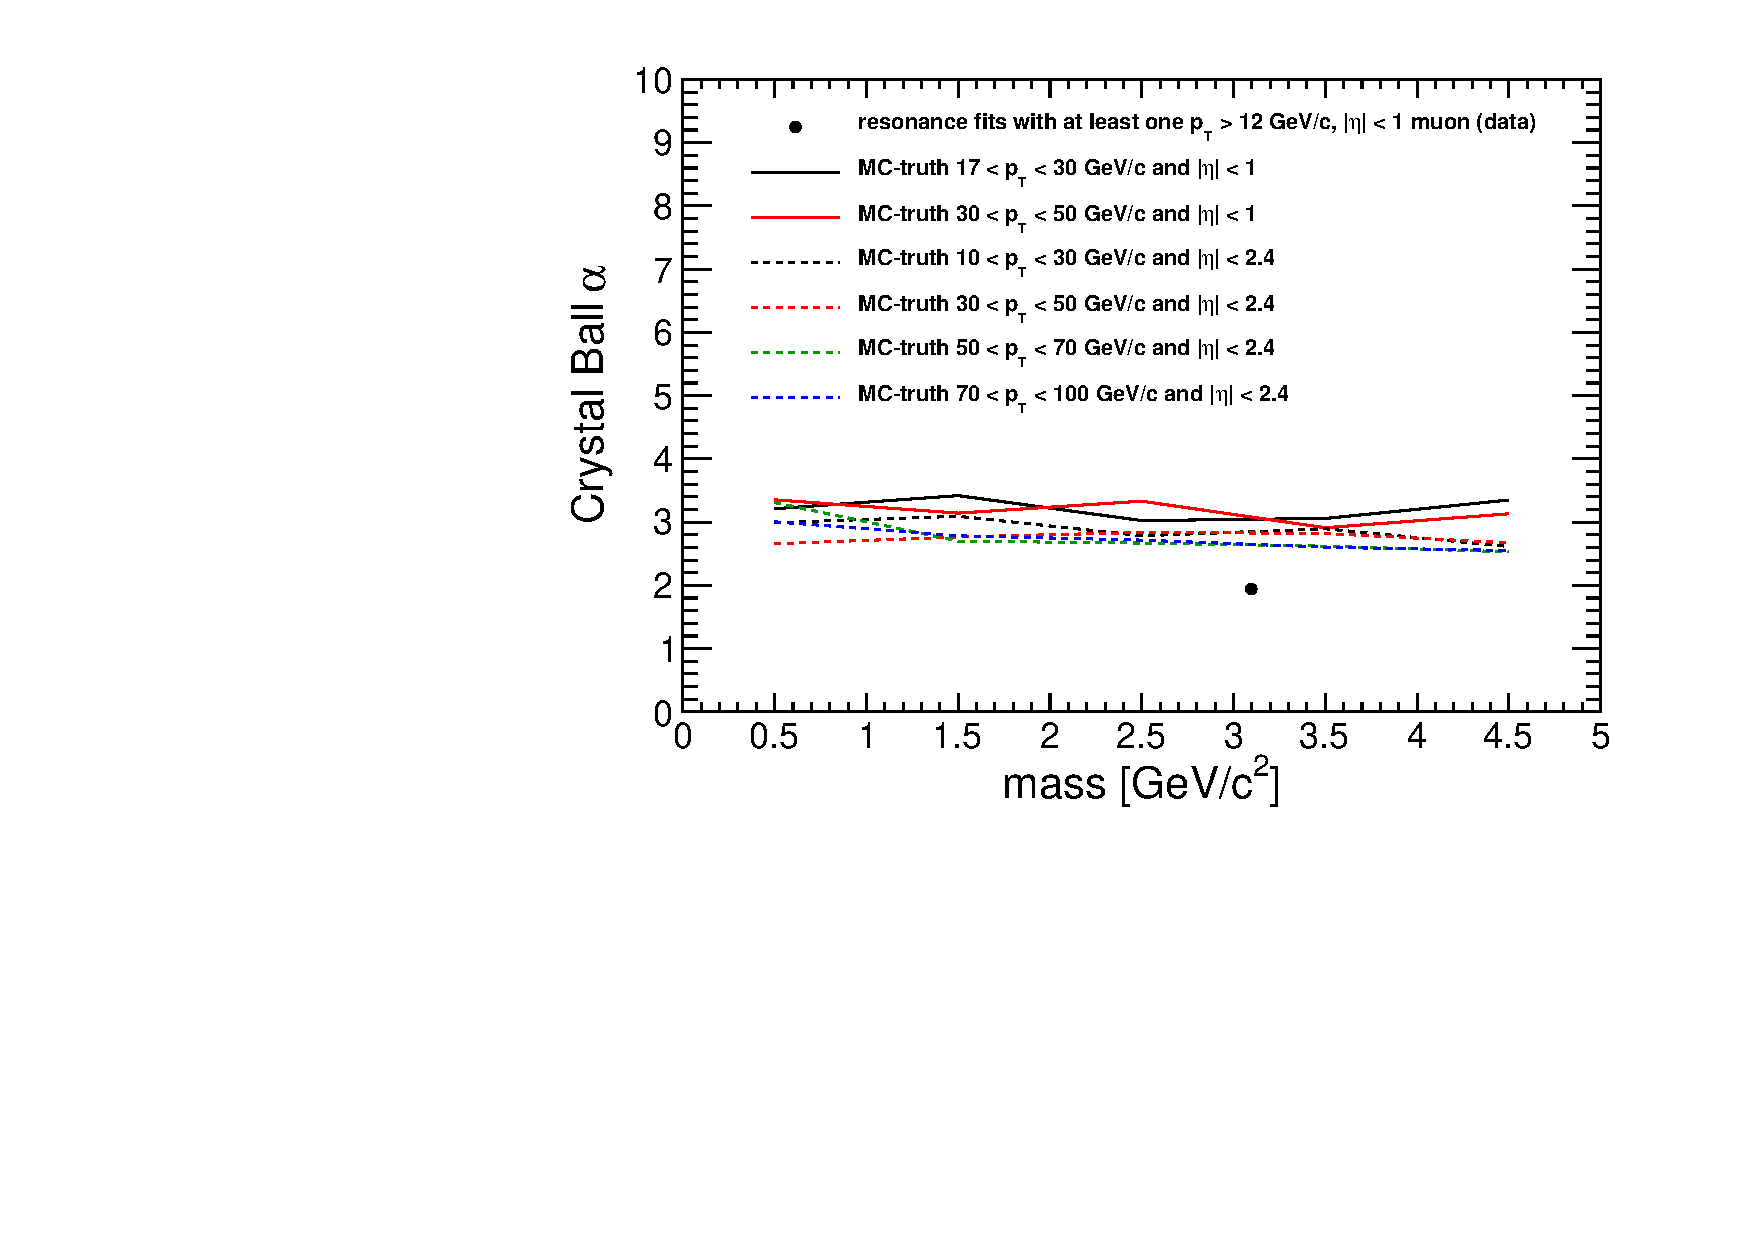
\includegraphics[width=0.5\linewidth]{resolution_alpha.pdf}

\item Two reasons to distinguish between the ``central'' dimuon
  (satisfying the trigger) and the ``other'' dimuon:
\begin{itemize}
\item slightly different background shapes
\item different signal resolutions
\end{itemize}
\end{itemize}
\end{frame}

%% \section*{First section}
%% \begin{frame}
%% \begin{center}
%% \Huge \textcolor{blue}{First section}
%% \end{center}
%% \end{frame}

\begin{frame}
\frametitle{Conclusions}
\begin{itemize}\setlength{\itemsep}{0.5 cm}
\item The physics models that inspired lepton jets searches are models
  of new resonances, conducive to ``bump hunts''

\item The hidden sector may be complicated, but if decays must pass
  through a lightest hidden state $m_1$, then all of the resulting
  muon pairs have the same invariant mass (unless they're
  misidentified)

\item Fitting that mass spectrum allows us to determine the
  backgrounds normalization in the same step, and we can get the
  shapes of those templates from the data, too
\end{itemize}
\label{numpages}
\end{frame}

\begin{frame}
\frametitle{Composition of inclusive MC}

\vspace{0.75 cm}
\hfill 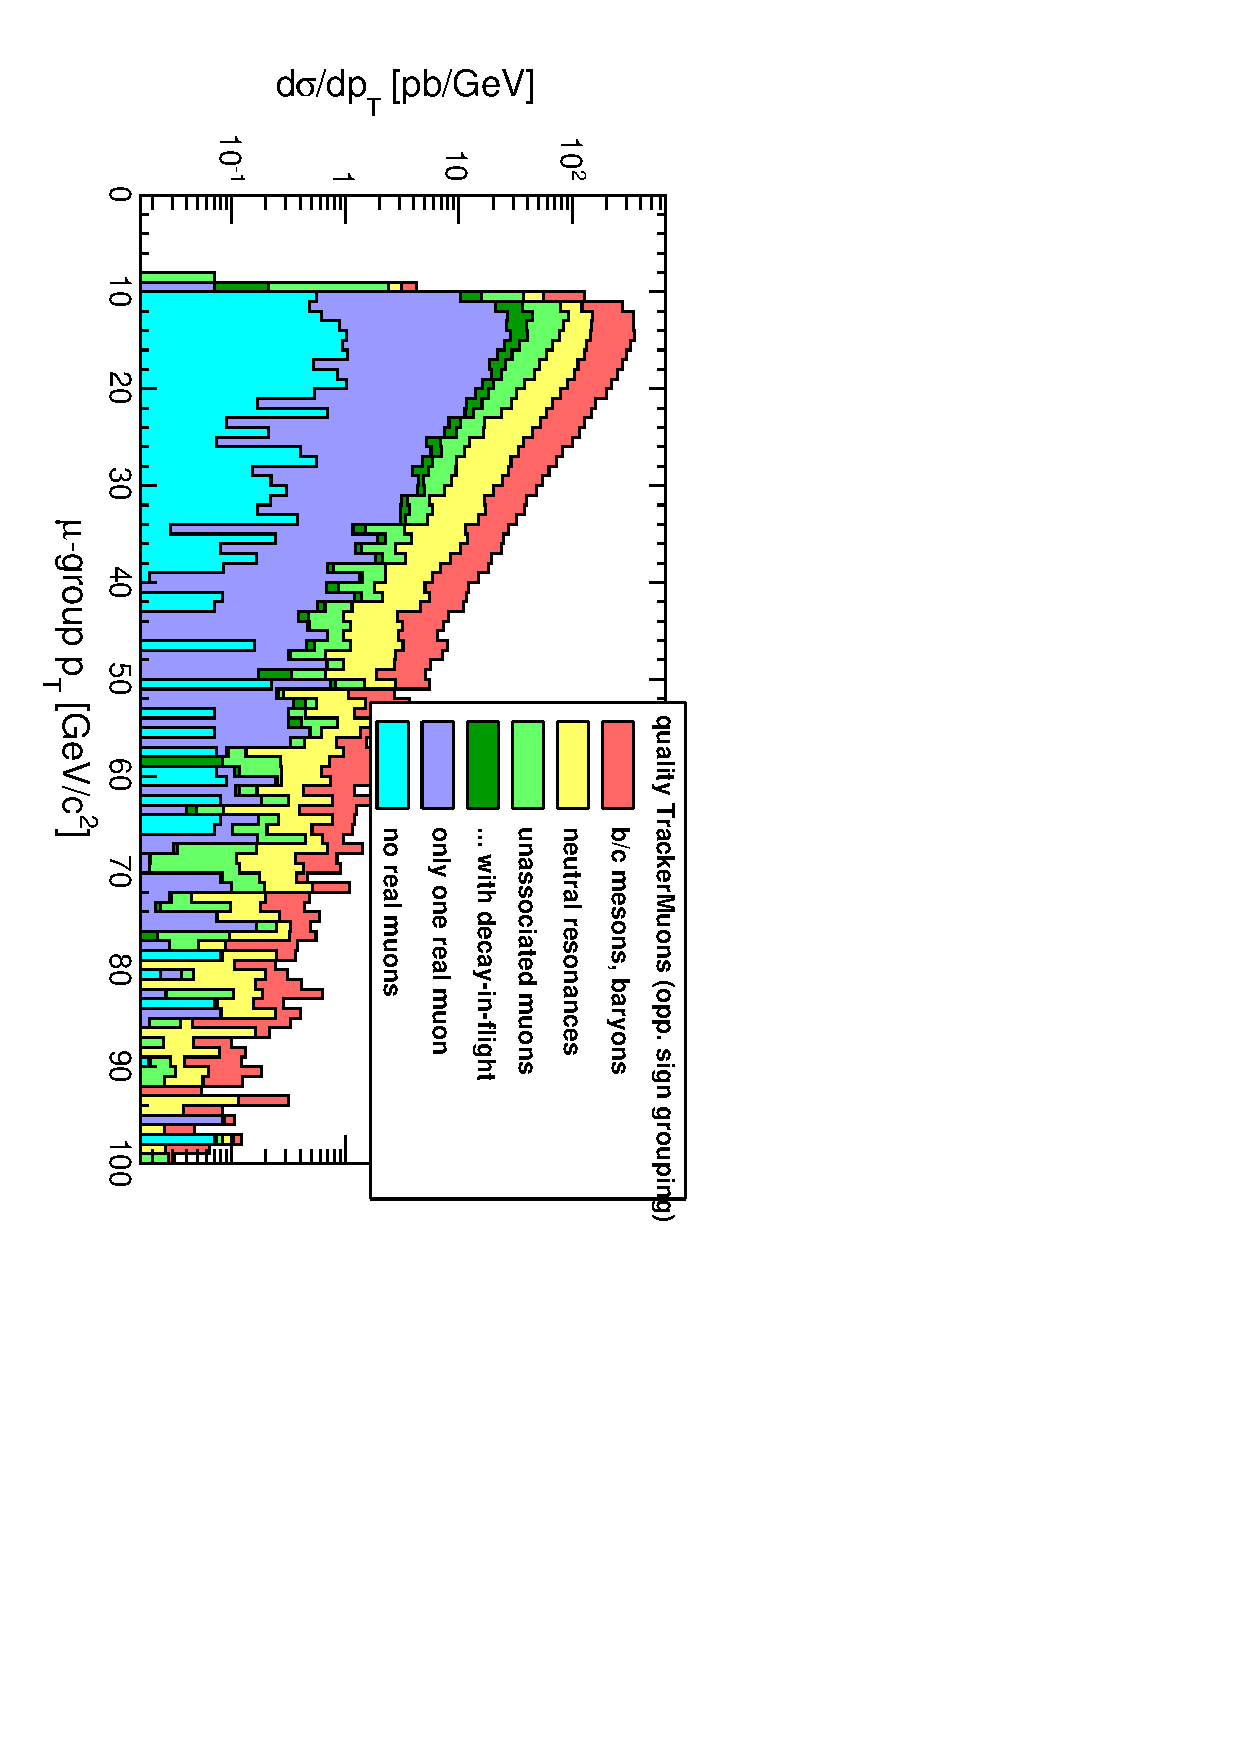
\includegraphics[height=0.5\linewidth, angle=90]{ptlog_QualityTrackerMuonOpposite.pdf}

\vspace{-3.3 cm}
\begin{itemize}
\item Plots of the inclusive-muon \\ sample, divided up by \\ generator-level information
\item Decays-in-flight and fakes are \\ simulated, but not significant
\end{itemize}

\vfill
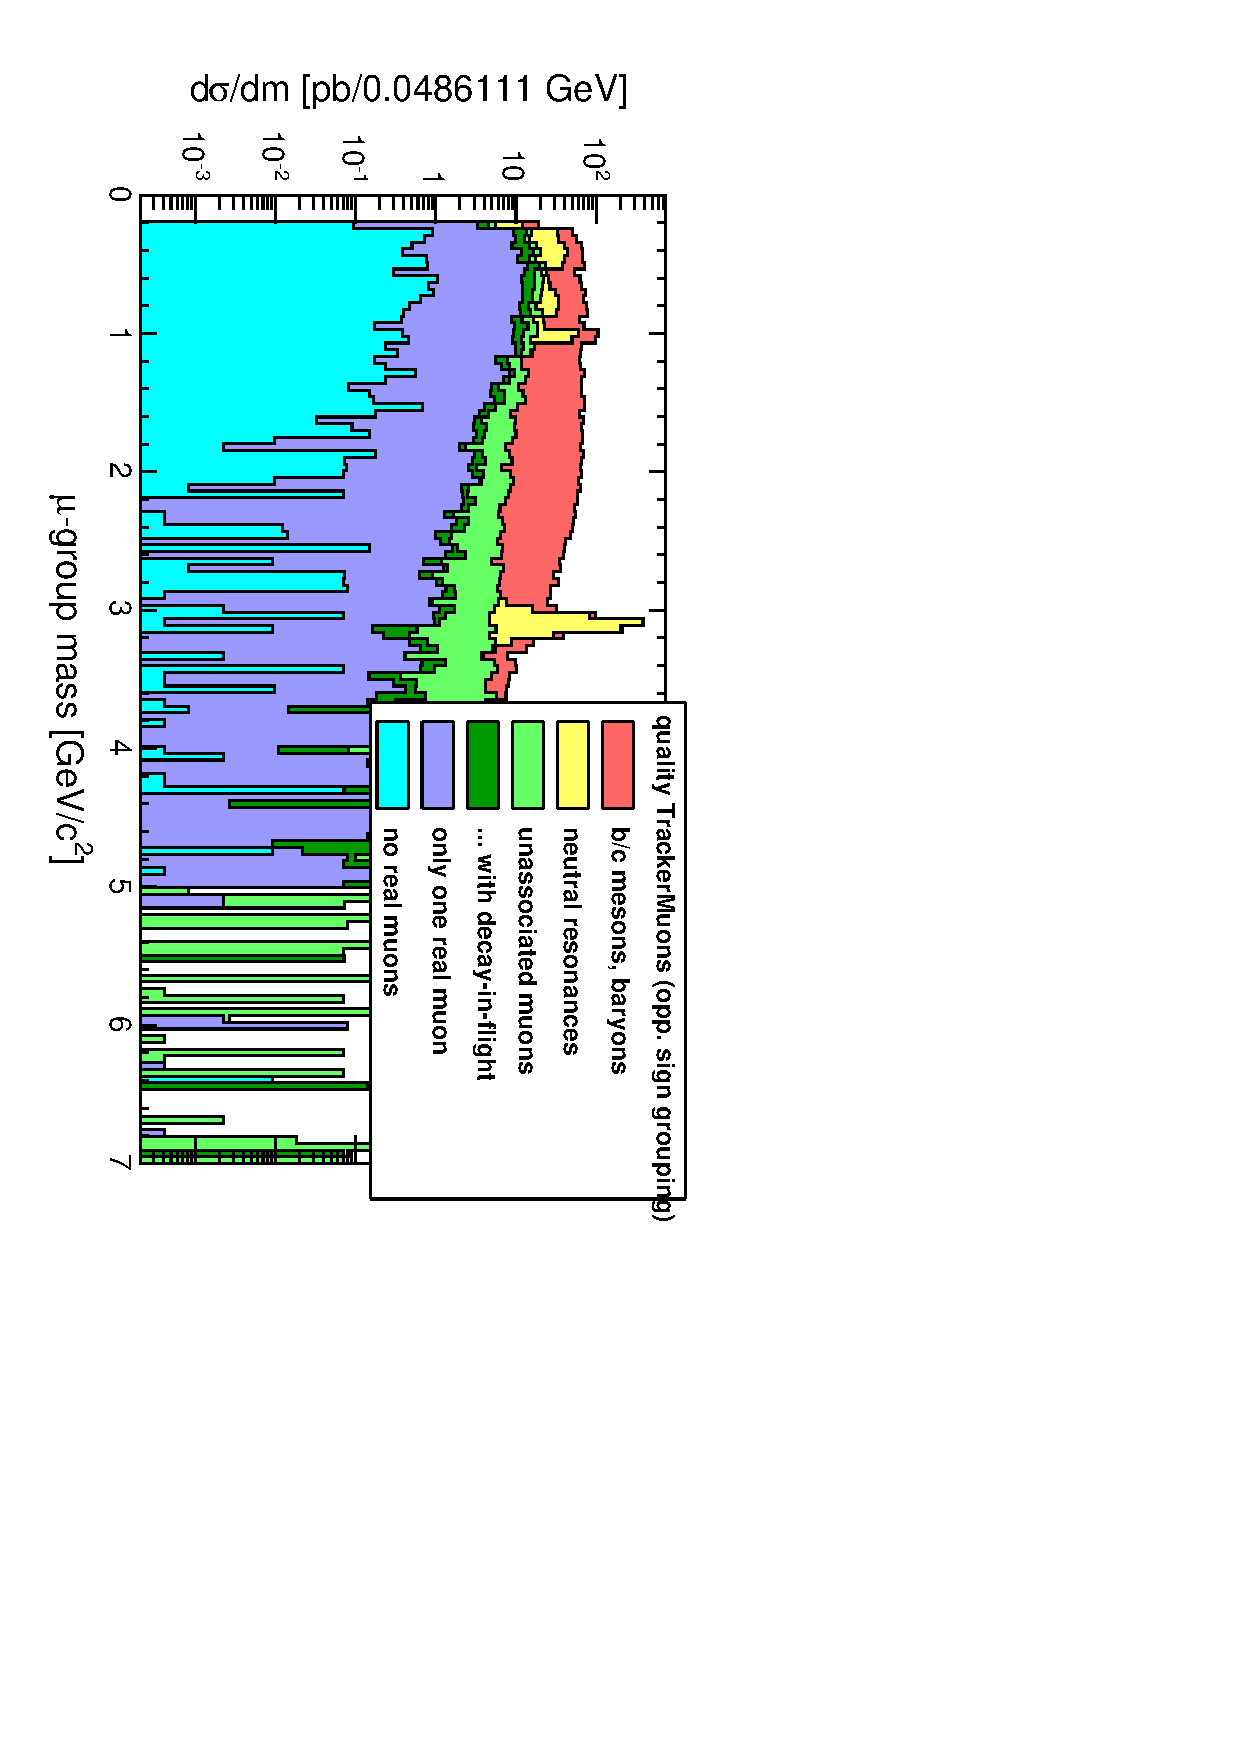
\includegraphics[height=0.5\linewidth, angle=90]{masslog_QualityTrackerMuonOpposite.pdf}
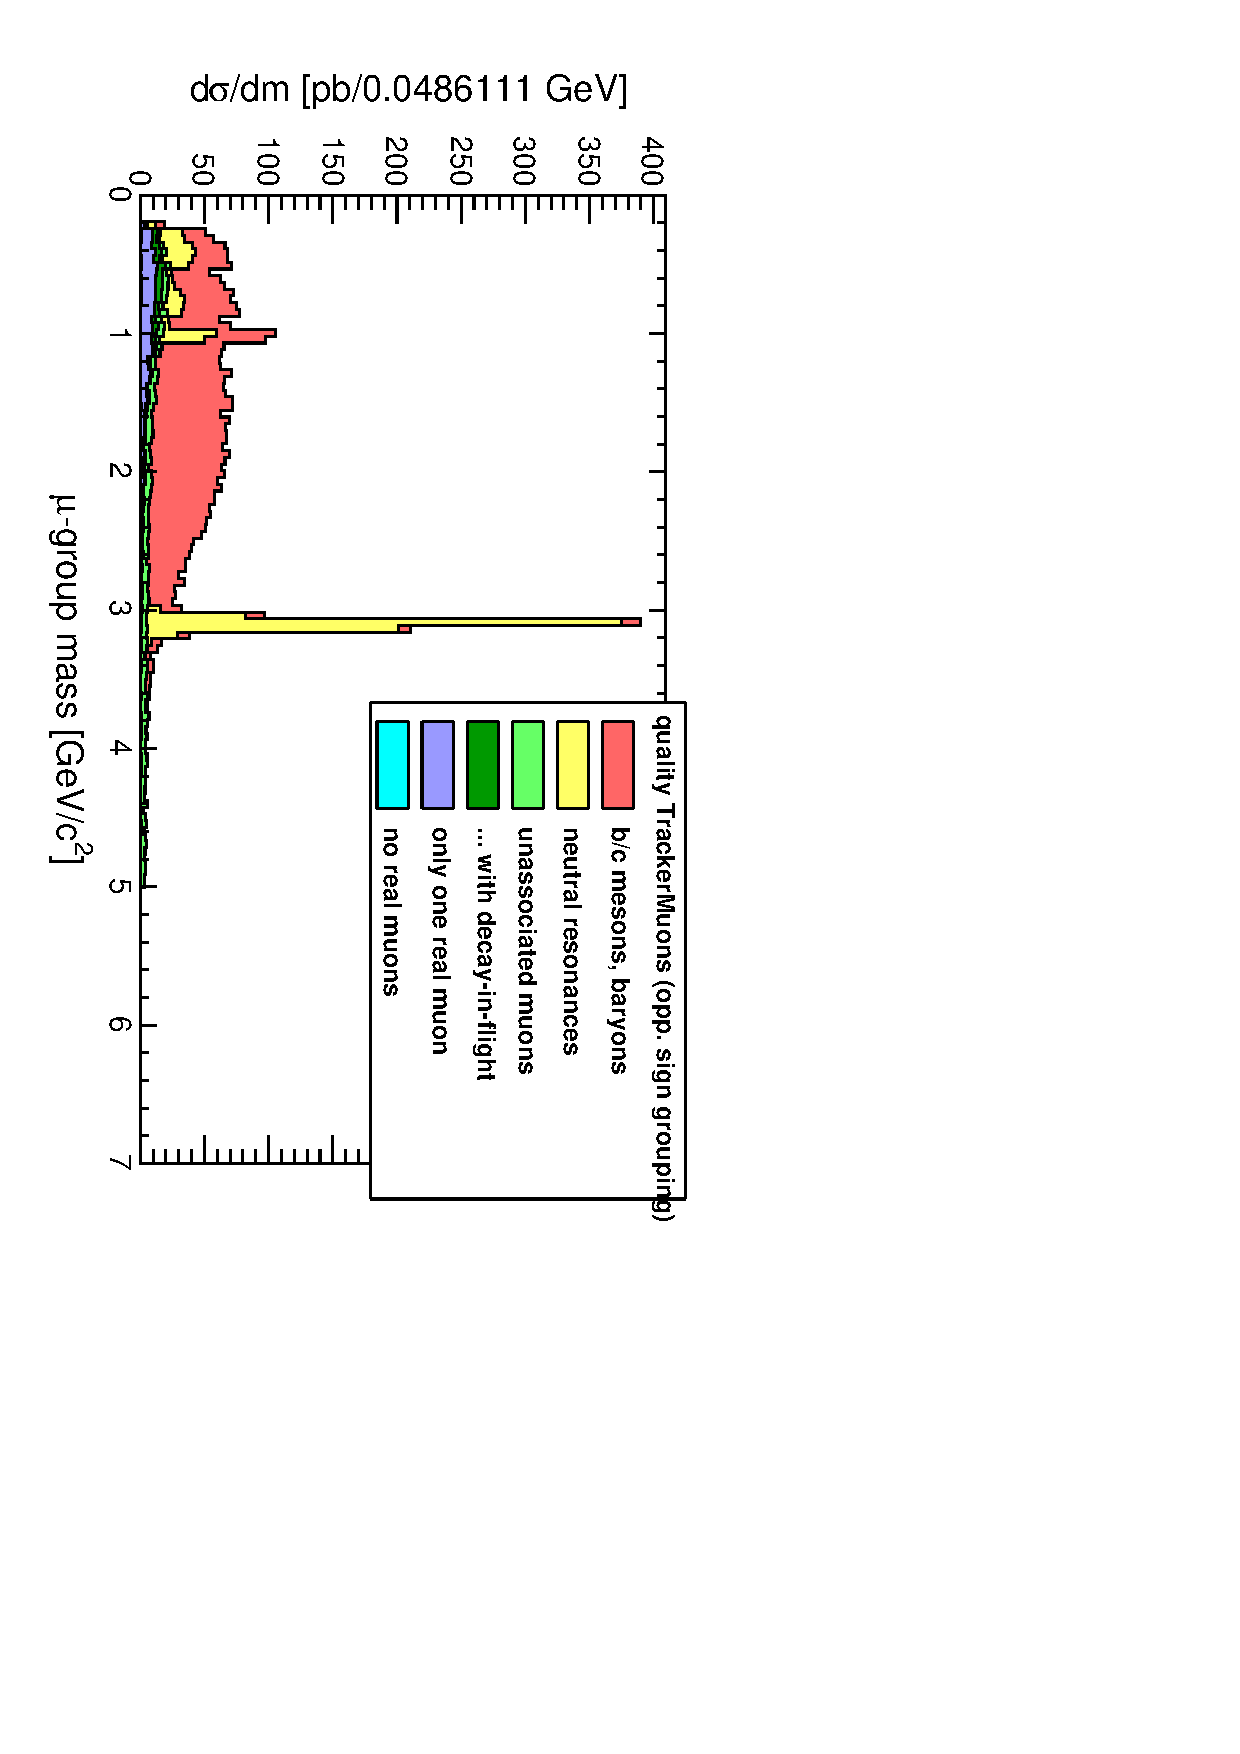
\includegraphics[height=0.5\linewidth, angle=90]{masslinear_QualityTrackerMuonOpposite.pdf}

\begin{itemize}
\item These are old plots (July), but they're perfectly relevant for a
  $p_T > 10$~GeV/$c$, $|\eta| < 2.4$ dimuon (no changes in cuts or clustering)
\end{itemize}
\end{frame}

\begin{frame}
\frametitle{Why require a barrel muon?}

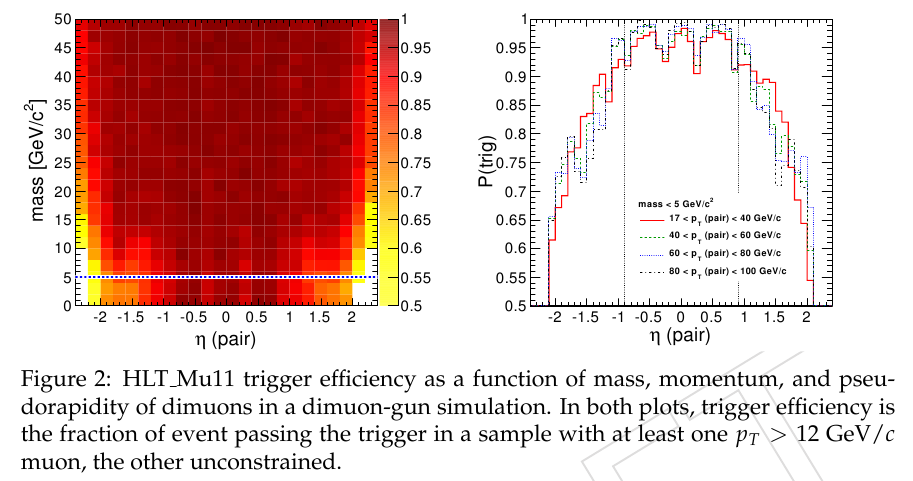
\includegraphics[width=\linewidth]{trigger_efficiency_loss1.png}
\end{frame}

\begin{frame}
\frametitle{Why require a barrel muon?}

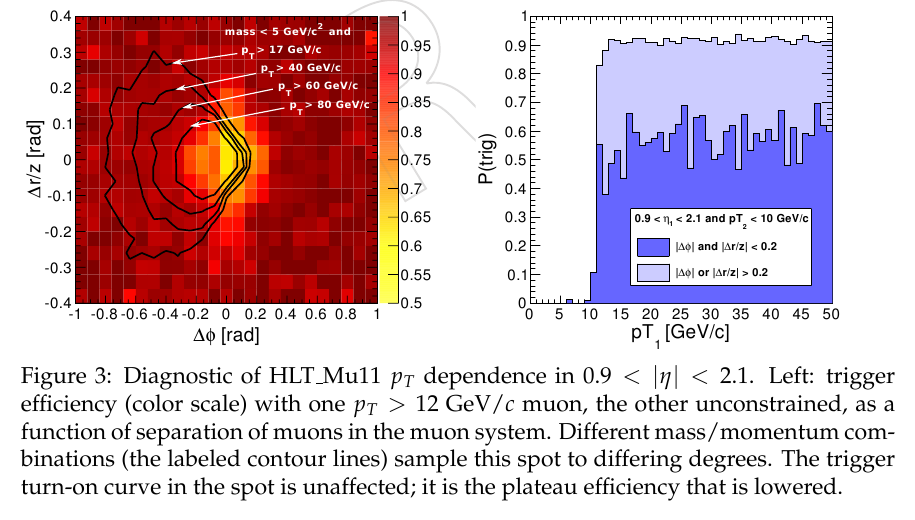
\includegraphics[width=\linewidth]{trigger_efficiency_loss2.png}
\end{frame}

\begin{frame}
\frametitle{Quality of low-mass dimuons}

\begin{columns}
\column{0.6\linewidth}
\begin{itemize}
\item Compare muon quality distributions in the mass $<$ 0.5~GeV/$c^2$
  region (black) with the same distributions in the $J/\psi$ peak
  (red)
\item Normalized to equal area (all data)
\end{itemize}

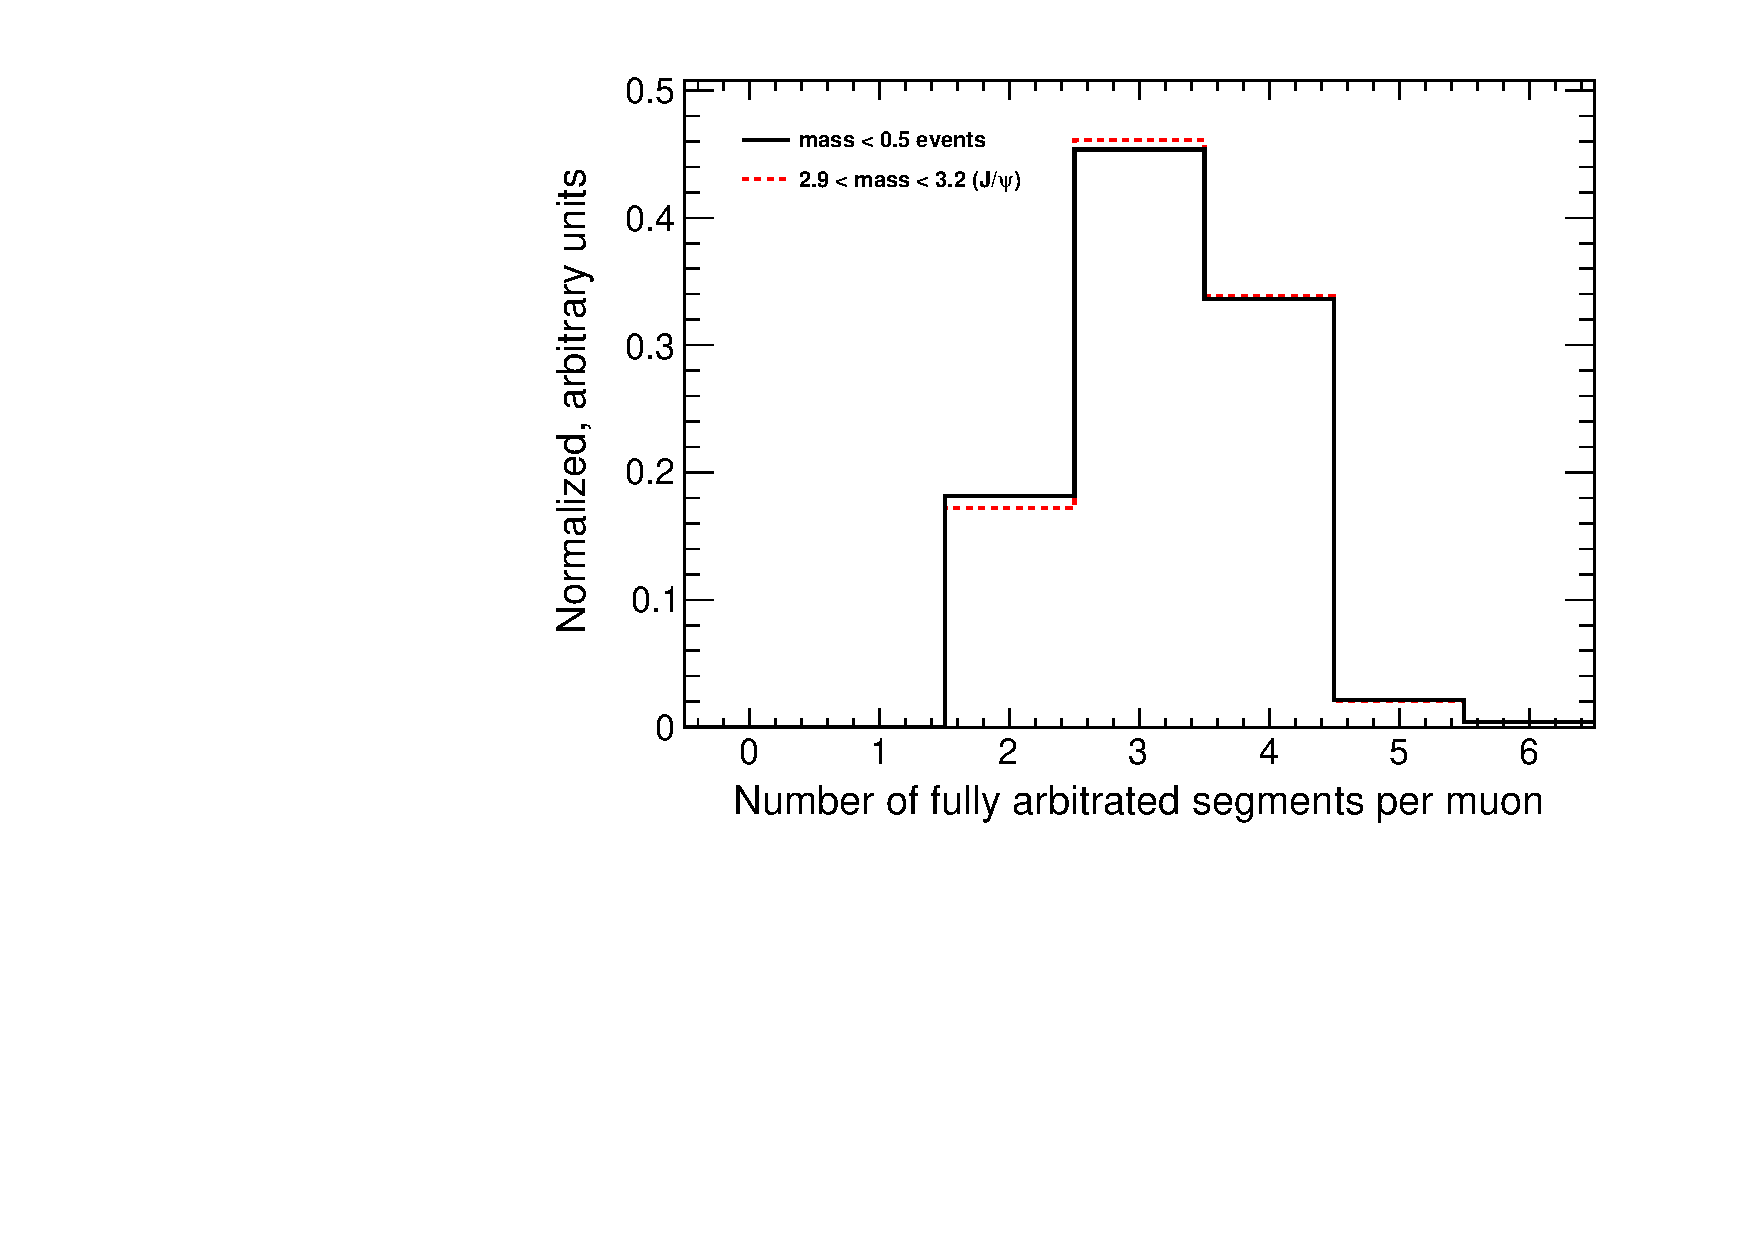
\includegraphics[width=\linewidth]{lowmassquality_matches.pdf}

\column{0.4\linewidth}
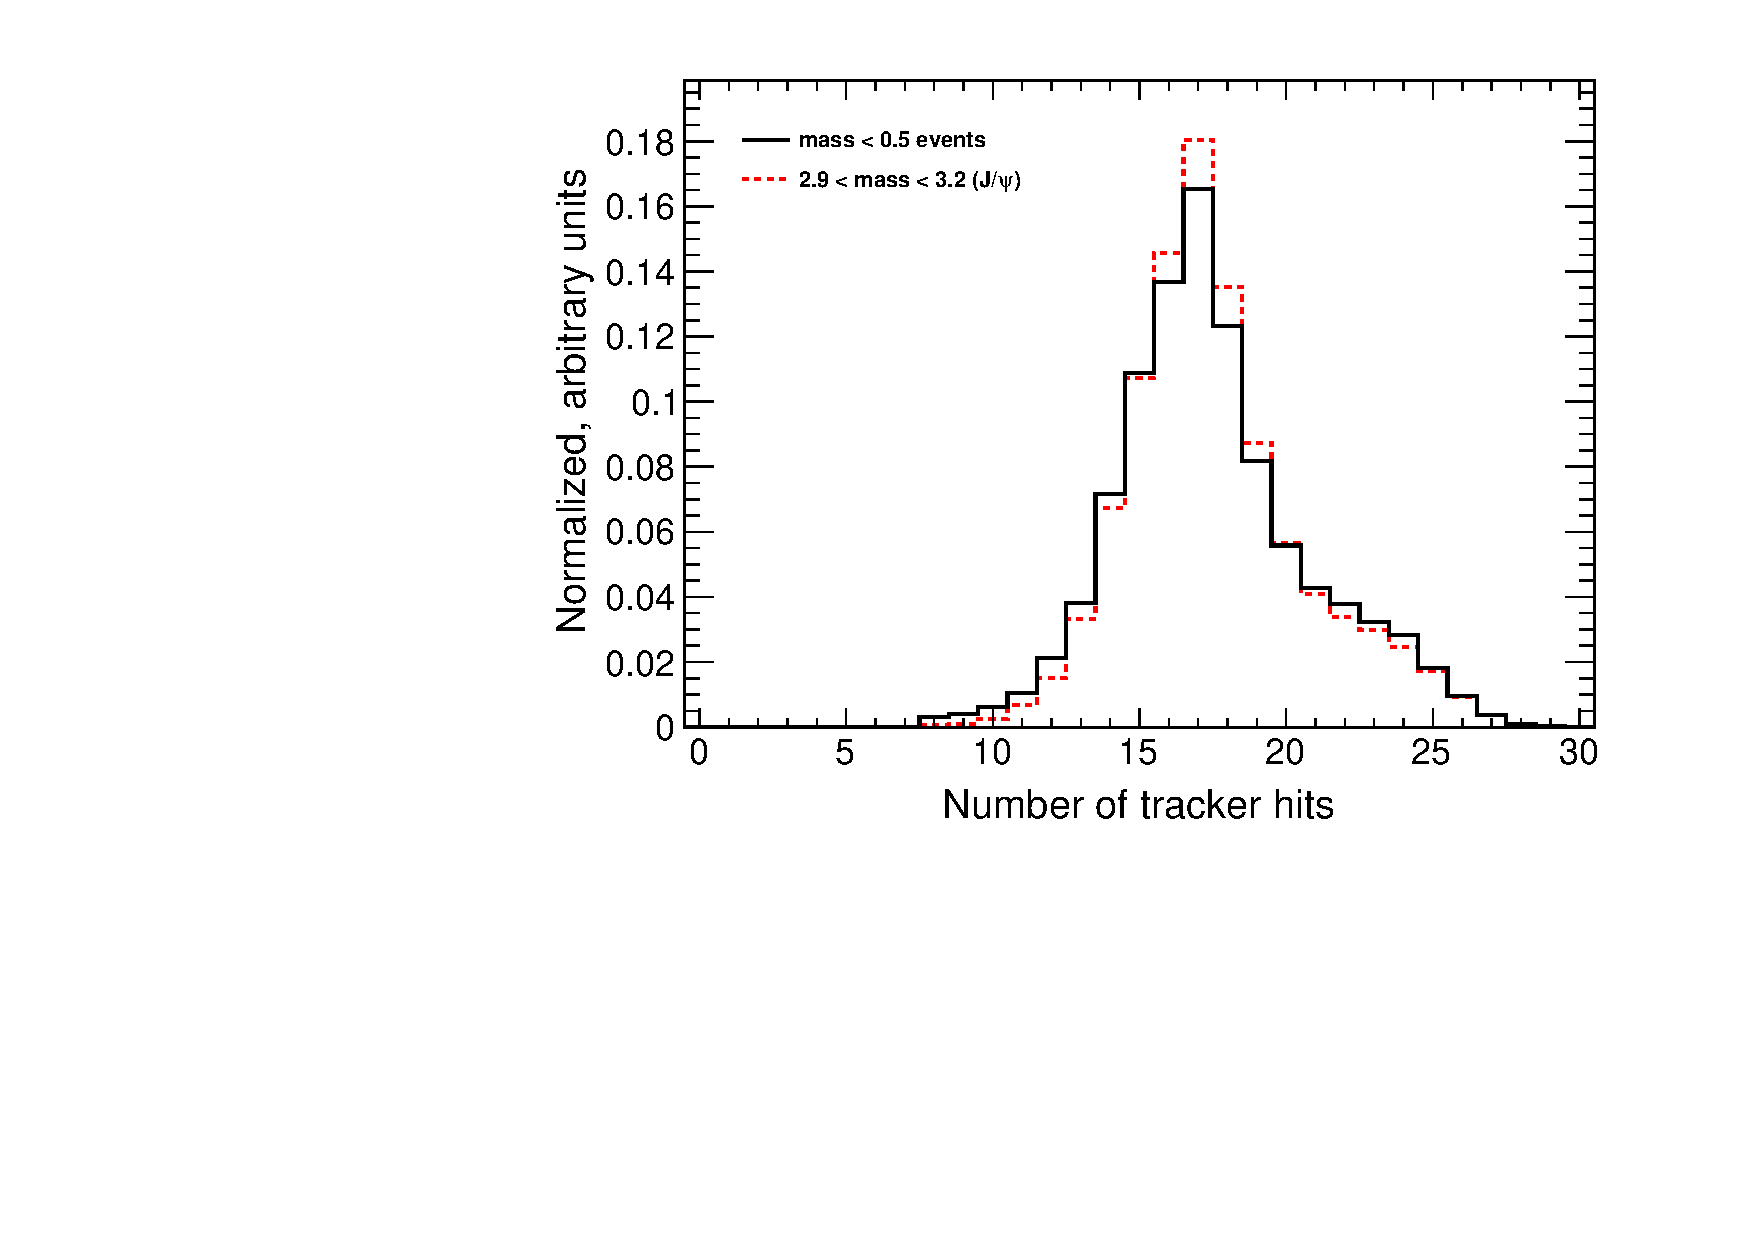
\includegraphics[width=\linewidth]{lowmassquality_hits.pdf}

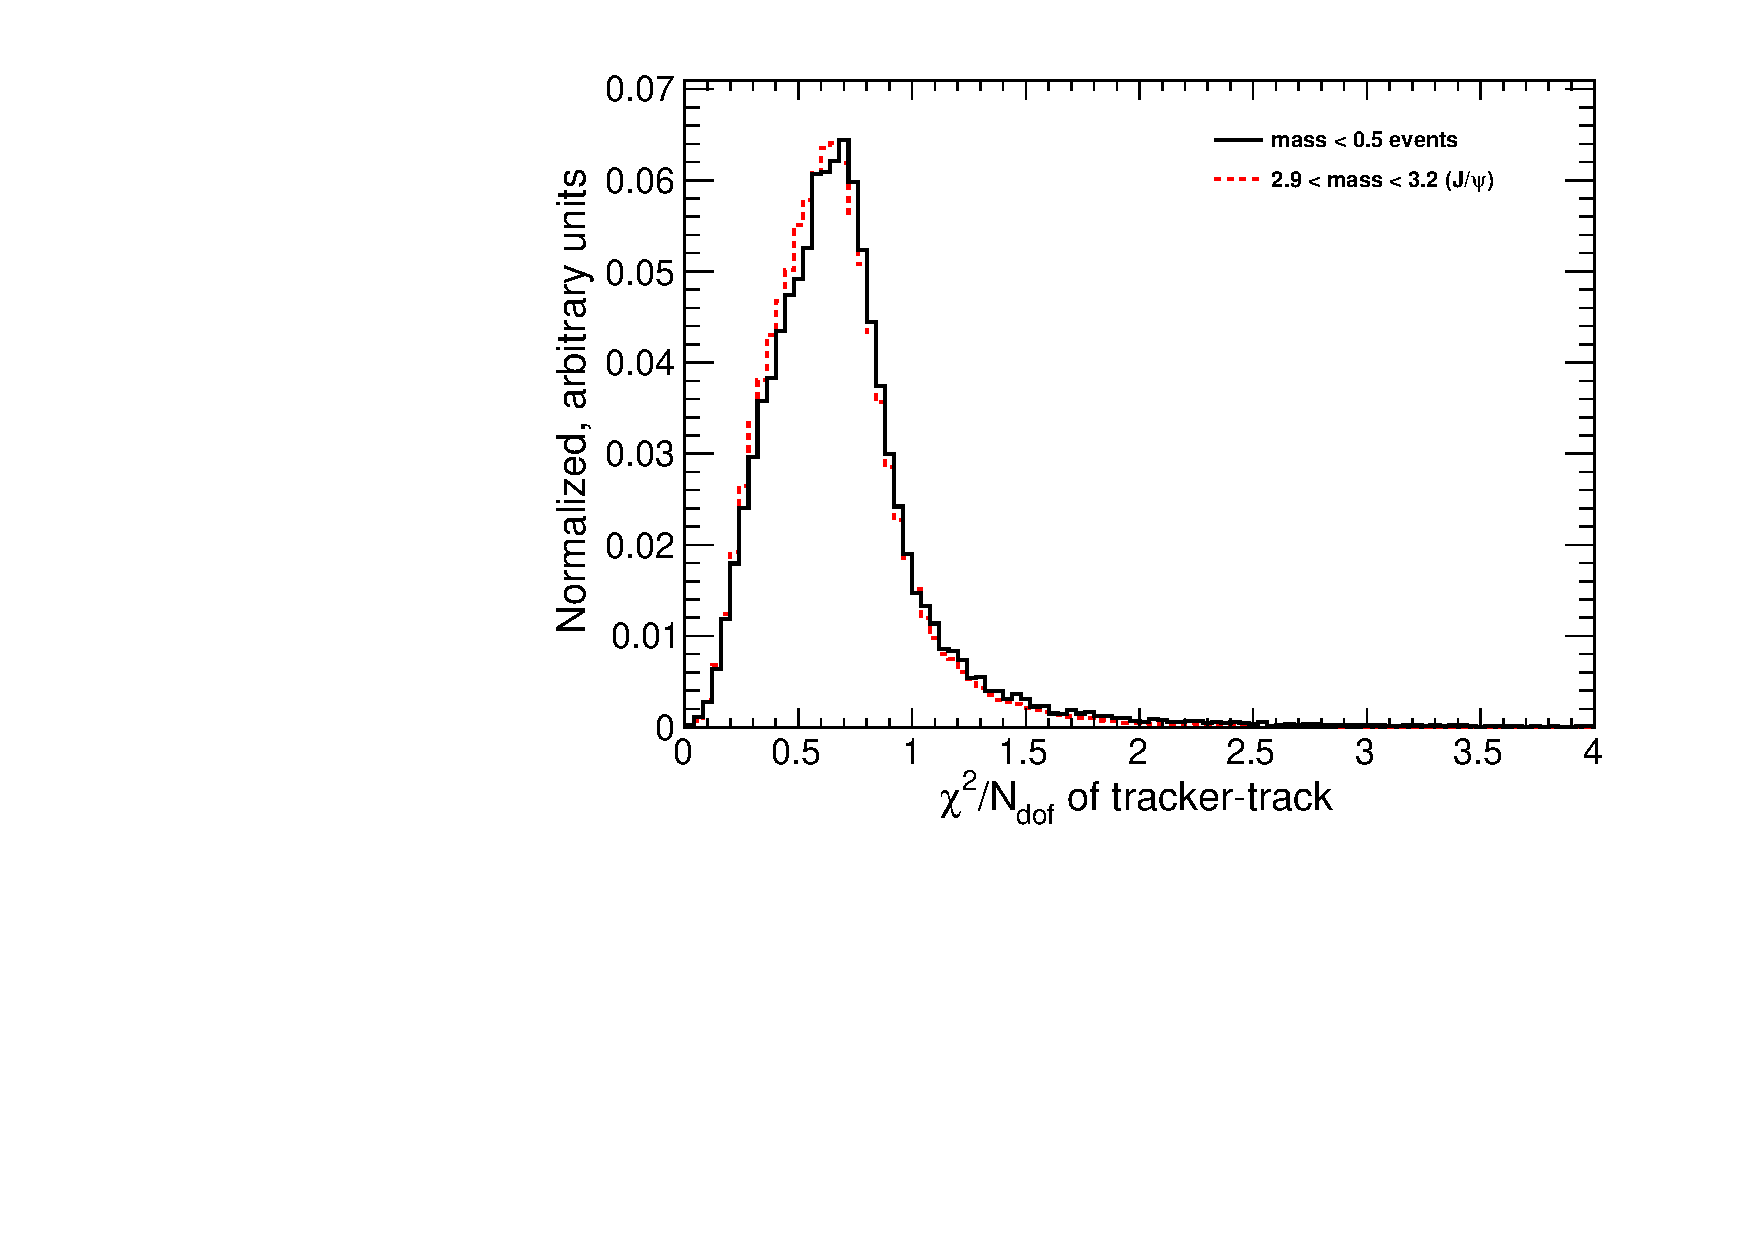
\includegraphics[width=\linewidth]{lowmassquality_normchi2.pdf}
\end{columns}
\end{frame}

\begin{frame}
\frametitle{Quality of low-mass dimuons}

\begin{itemize}
\item Residuals distributions in station 1 (of both barrel and endcap)
\end{itemize}

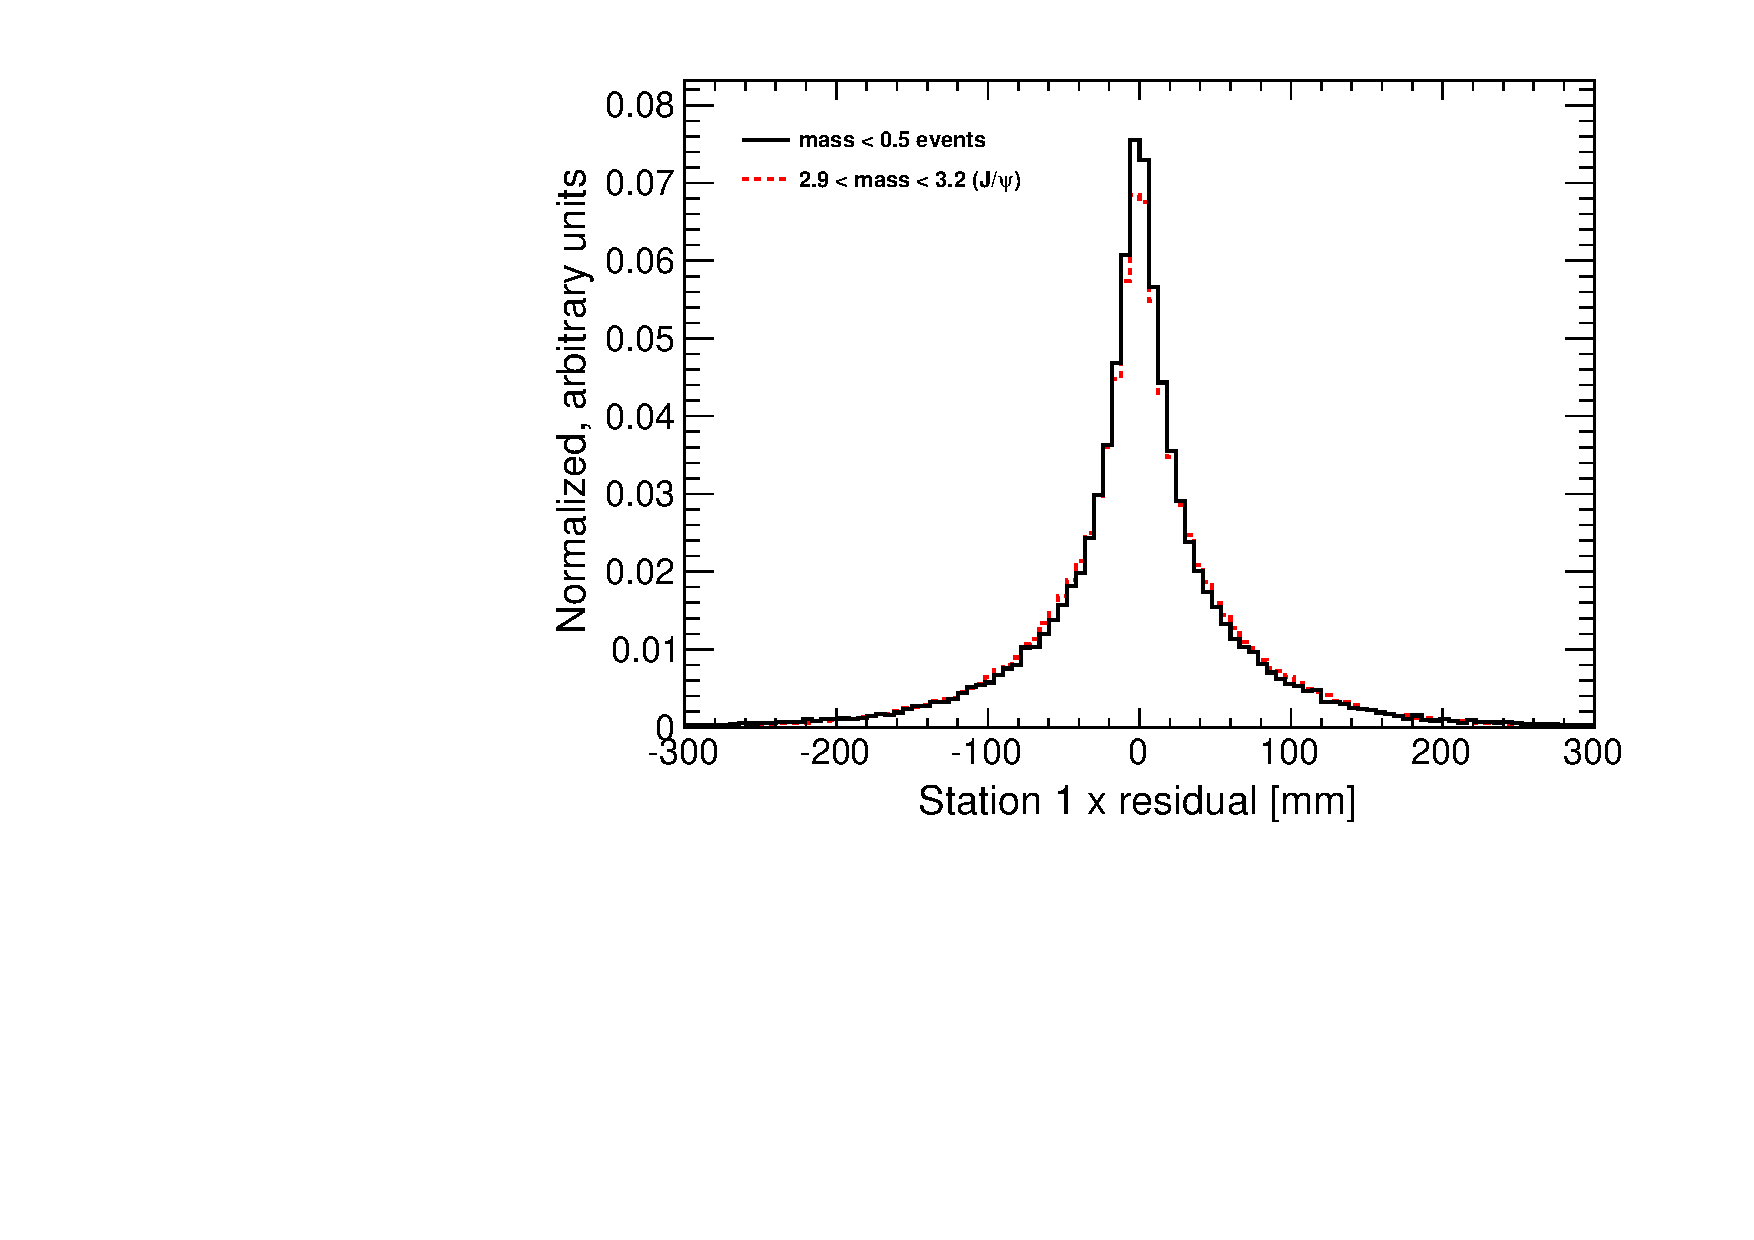
\includegraphics[width=0.45\linewidth]{lowmassquality_st1x.pdf} \hfill
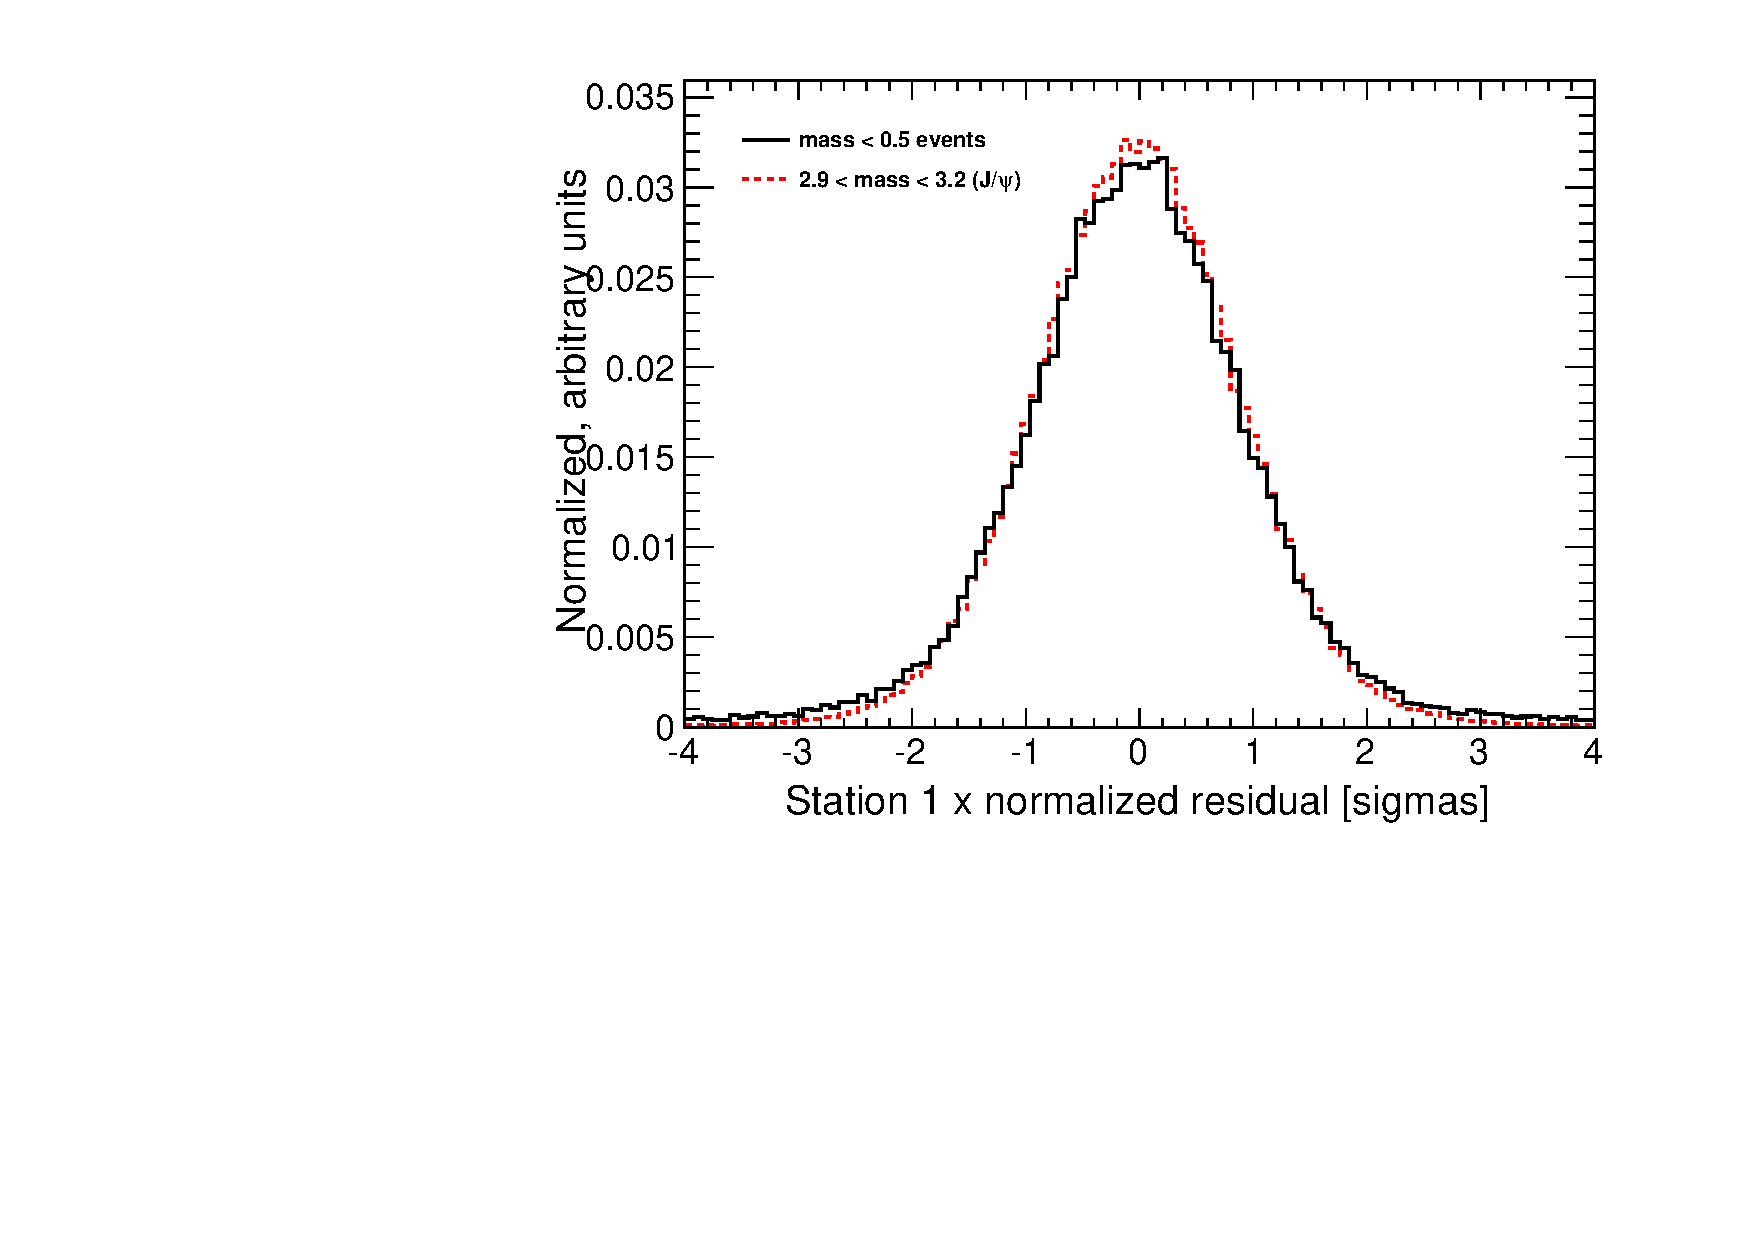
\includegraphics[width=0.45\linewidth]{lowmassquality_st1xsig.pdf}

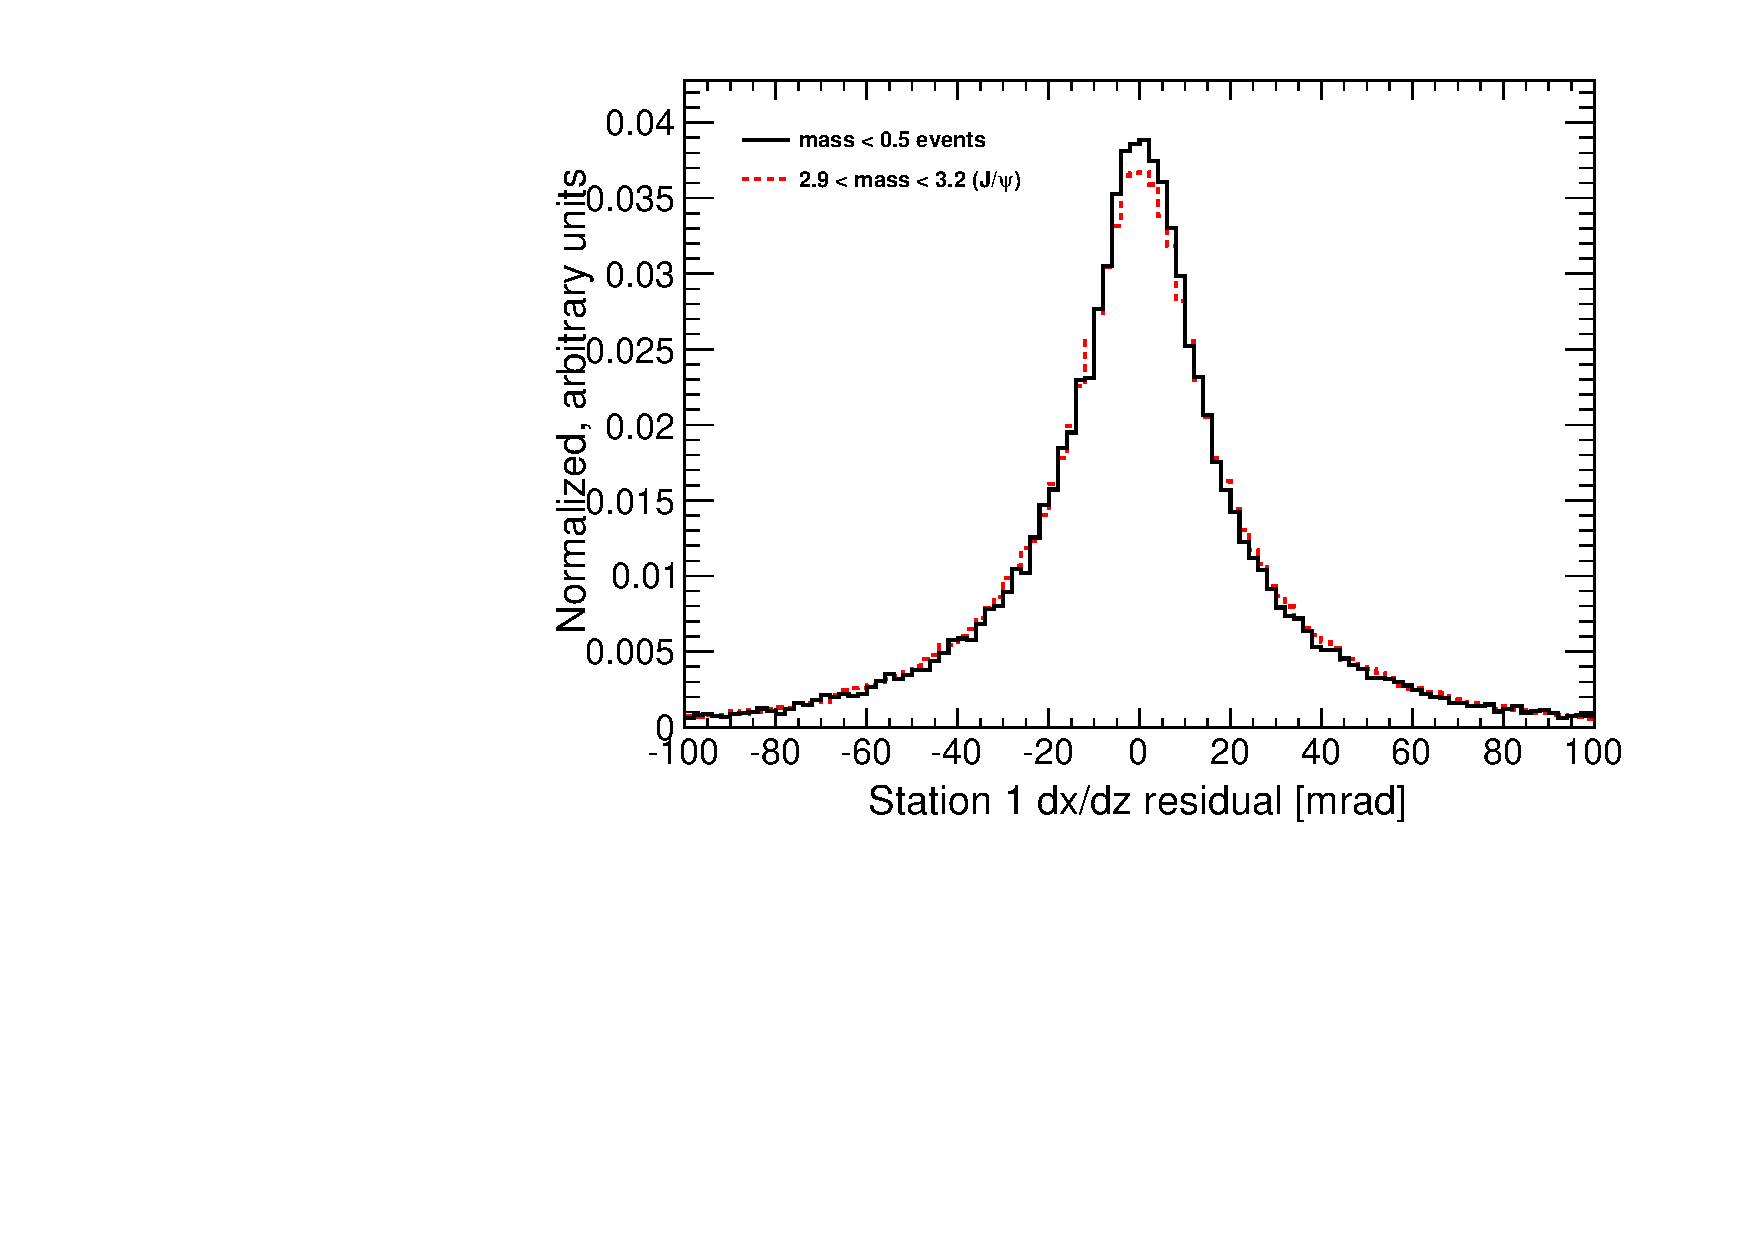
\includegraphics[width=0.45\linewidth]{lowmassquality_st1dxdz.pdf} \hfill
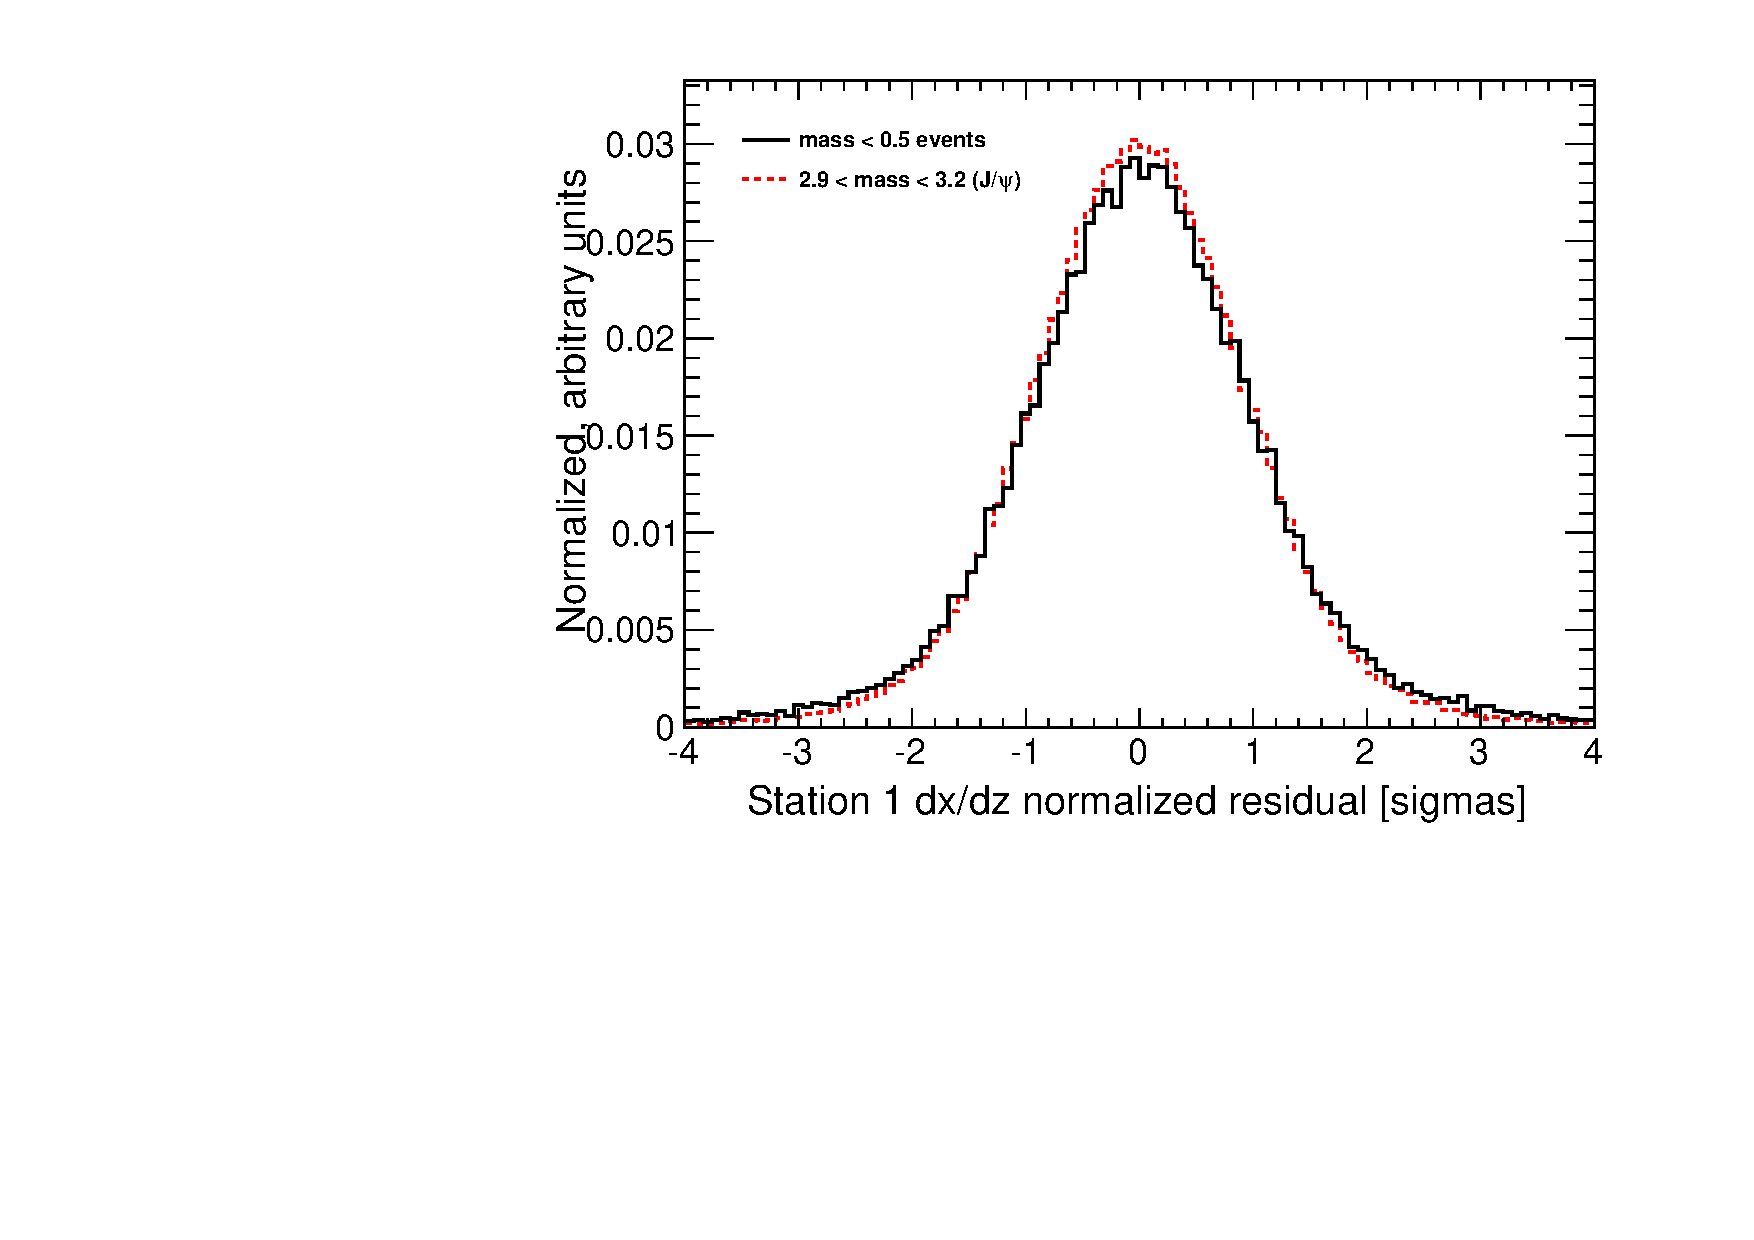
\includegraphics[width=0.45\linewidth]{lowmassquality_st1dxdzsig.pdf}
\end{frame}

\end{document}
